\documentclass[12pt,svgnames,table]{beamer}
\usetheme{progressbar}
%\usetheme{onerajdt}


\usepackage[utf8x,utf8]{inputenc}
\usepackage{tikz}
\usetikzlibrary{decorations.pathmorphing}
\usepackage{xcolor}
\usepackage{amsmath,amsfonts,amsthm, amssymb}
\usepackage[babel=true]{csquotes}
\usepackage{etoolbox}
\usepackage{dsfont}
\usepackage{chngpage}


\usepackage{graphics} %% TOUT NEW!!
\usepackage{pgfplots} %% TOUT NEW!!  virer si pbm

\usetikzlibrary{shapes,snakes}

%\usepackage{txfonts}
%\usepackage{MnSymbol} % symbol independent
\newcommand{\paren}[1]{\left( \left. #1 \right. \right)} 
\newcommand{\croch}[1]{\left[ \left. #1 \right. \right]} 
\newcommand{\set}[1]{\left\{ \left. #1 \right. \right\}}
\newcommand{\sachant}{\, \right| \left. \,}
\newcommand{\nico}[1]{ }
\newcommand{\nicoo}[1]{#1}
% Modifiez ou necessaire:
% titre de these/topo

\title{
\vspace{0.7cm}\\
Exploiting Imprecise Information Sources\\
in Sequential Decision Making Problems\\
under Uncertainty}

\normalsize
\author{\vspace{0.1cm} \textbf{N.Drougard}}
% X=annee de these, Y=departement
\def\aboutauthor{\vspace{0.2cm}\hspace{-2.55cm} under \textbf{D.Dubois}, \textbf{J-L.Farges} and \textbf{F.Teichteil-K\"onigsbuch} supervision\\
\vspace{0.1cm}\hspace{-2.4cm} \textbf{doctoral school:} EDSYS \hspace{0.2cm} \textbf{institution:} ISAE--SUPAERO\\
\vspace{0.1cm}\hspace{-3.2cm}\textbf{laboratory:} ONERA--The French Aerospace Lab\\ 
\vspace{0.5cm} \hspace{0.2cm} 
\includegraphics[scale=0.45]{logo2015} \hspace{4.8cm}
\begin{tikzpicture}
\node[opacity=0.2] at (0,0) {
\includegraphics[scale=0.35]{Logo_EDSYS2}};
\end{tikzpicture}
}

% directeur de these
%\def\directeur{Toulouse}
% encadrant; s'il n'y a pas d'encadrant, veuillez commenter la ligne ci-dessous
%\def\encadrant{DCSD}


% Debut du documment
\begin{document}

% la premiere page
{
\usebackgroundtemplate{
\includegraphics[width=\paperwidth,height=\paperheight]{beamer-onera-background}} 
\begin{frame}[plain]
	\titlepage
\end{frame}
}


%%%%%%%%%%%%%%%%%%%%%%%%%%%%%%%%%%%%%%%%%%%%%%%%%%
%%%%%%%%%%%%%%%%%%%%%%%%%%%%%%%%%%%%%%%%%%%%%%%%%%
%%%%%%%%%%%%%%%%%%%%%%%%%%%%%%%%%%%%%%%%%%%%%%%%%%
%%%%%%%%%%%%%%%%%%%%%%%%%%%%%%%%%%%%%%%%%%%%%%%%%%
%%%%%%%%%%%%%%%%%%%%%%%%%%%%%%%%%%%%%%%%%%%%%%%%%%
%%%%%%%%%%%%%%%%%%%%%%%%%%%%%%%%%%%%%%%%%%%%%%%%%%
%%%%%%%%%%%%%%%%%%%%%%%%%%%%%%%%%%%%%%%%%%%%%%%%%%
%%%%%%%%%%%%%%%%%%%%%%%%%%%%%%%%%%%%%%%%%%%%%%%%%%
%%%%%%%%%%%%%%%%%%%%%%%%%%%%%%%%%%%%%%%%%%%%%%%%%%
%%%%%%%%%%%%%%%%%%%%%%%%%%%%%%%%%%%%%%%%%%%%%%%%%%
%%%%%%%%%%%%%%%%%%%%%%%%%%%%%%%%%%%%%%%%%%%%%%%%%%
%%%%%%%%%%%%%%%%%%%%%%%%%%%%%%%%%%%%%%%%%%%%%%%%%%
%%%%%%%%%%%%%%%%%%%%%%%%%%%%%%%%%%%%%%%%%%%%%%%%%%
%%%%%%%%%%%%%%%%%%%%%%%%%%%%%%%%%%%%%%%%%%%%%%%%%%
%%%%%%%%%%%%%%%%%%%%%%%%%%%%%%%%%%%%%%%%%%%%%%%%%%
\nico{

% La premiere planche
% Ci-dessous c'est a vous de remplir
\section[context]{Context}

\begin{frame}
\frametitle{\insertsection} 
\framesubtitle{\footnotesize Autonomous robotics } 
\normalsize
\begin{block}{Onera, Flight Dynamics $\&$ System control}
Control Engineering, Artificial intelligence, Cognitive Sciences
\end{block}
\vspace{0.5cm}
\visible<2->{
\begin{minipage}{0.53\linewidth}
among many other works:
\begin{itemize}
\item autonomy and\\ human factors
\item decision making, planning
\item experimental/industrial applications:
UAVs,\\ 
human-machine interaction,\\
exploration robots
\end{itemize}
\end{minipage}
\begin{minipage}{0.42\linewidth}
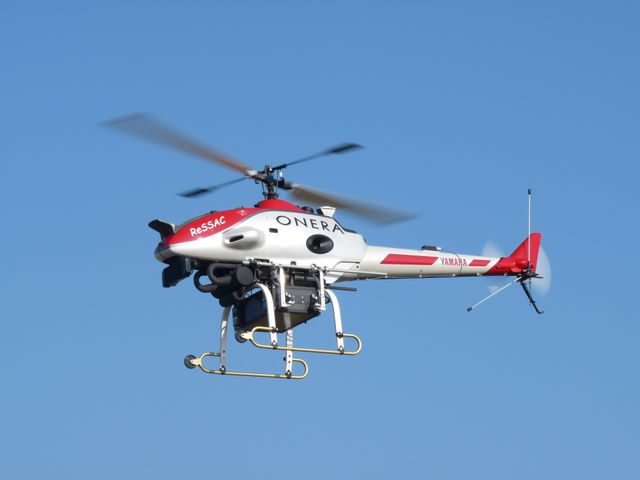
\includegraphics[scale=0.23]{ReSSAC_vol}
\end{minipage}
}
\end{frame}



\begin{frame}
\frametitle{\insertsection} 
\framesubtitle{\footnotesize Partially Observable Markov Decision Processes (POMDPs)} 
\normalsize
\vspace{-0.5cm}
\begin{tikzpicture}[scale=0.9,transform shape]
\vspace{0.2cm}
\visible<1->{
\node (pomdp) at (3.5,5.6) {\textbf{POMDP:} model for autonomous robotics};
\node (rpomp) at (-1,4.7) {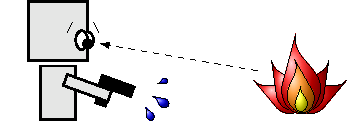
\includegraphics[scale=0.9]{robot_pompier}};
\node (bli) at (0,6.5) {};
}
\visible<2->{
\node (pomdp3) at (4.25,5.05) {\color{DodgerBlue!70}{$s \in \mathcal{S}$}: \color{black}{\textbf{system states}}};
\node (t1) at (2.3,5.05) {};
\node (r1) at (-1.05,5.5) {};
\node (r11) at (1.55,4.6) {};
\draw[color=DodgerBlue!70,thick] (t1) to (r1);
\draw[color=DodgerBlue!60,thick] (t1) to (r11);
\draw[color=DodgerBlue!60,thick] (-3.4,3.8) rectangle (-0.9,5.8);
\draw[color=DodgerBlue!60,thick] (0.15,3.85) rectangle (1.7,5);
}
\visible<3->{
\node (pomdp4) at (4.85,4.45) {\color{MediumAquamarine}{$o \in \mathcal{O}$:} \color{black} \textbf{system observations}};
\node (t2) at (2.3,4.5) {};
\node (r2) at (-2.15,4.95) {};
\draw[color=MediumAquamarine,thick] (t2) to[bend left] (r2);
\draw[color=MediumAquamarine,thick] (-2.33,5.07) circle (0.39cm);
}
\visible<4->{
\node (pomdp5) at (4.4,3.85) {\color{MediumPurple}{$a \in \mathcal{A}$:} \color{black} \textbf{agent's actions}};
\node (t3) at (2.3,3.9) {};
\node (r3) at (-1.2,4) {};
\draw[color=MediumPurple,thick] (t3) to[bend left] (r3);
\draw[color=MediumPurple,thick] (-1.4,4.2) circle (0.45cm);
}
\visible<12->{
\node (pomdp6) at (4.95,3.25) {\color{red}{$b$} \textbf{belief}: \color{black} \textbf{probability distribution} };
}
\end{tikzpicture}



\begin{tikzpicture}[scale=0.8,transform shape]
%%%%%%%%%%%%%%%%%%%%%%%%%%%%%%%%%%%%%%%%%%%%%%%%%%%%%%%%%%%%%%%%%%%%%%%%
%vis1: state
%%%%%%%%%%%%%%
%%%%%%%%%%%%%%
%\node (bli) at (0,0.5) {};
\visible<5->{
\tikzstyle{mvertex}=[circle,fill=DodgerBlue!70,minimum size=30pt,inner sep=0pt]
\tikzstyle{overtex}=[circle,fill=MediumAquamarine,minimum size=30pt,inner sep=0pt]
\tikzstyle{avertex}=[fill=MediumPurple,minimum size=20pt,inner sep=0pt]

\node[mvertex] (state1t) at (3,0) {$s_t$};
}
%vis2 action
%%%%%%%%%%%%%%
%%%%%%%%%%%%%%
\visible<6->{
\node[avertex] (action) at (6.3,-1.7) {$a_t$};
}
%vis3: next state
%%%%%%%%%%%%%%
%%%%%%%%%%%%%%
\visible<7->{
\node[mvertex] (state2t) at (7.7,0) {$s_{t+1}$};
\tikzstyle{bvertex}=[circle,fill=red!60,minimum size=30pt,inner sep=0pt]
%1->2
\draw[->,>=latex] (state1t) -- (state2t);
\draw[->,>=latex] (action) -- (state2t);
\node (pisasp) at (6,-0.3) {$\textbf{p} \hspace{-0.05cm} \paren{ \hspace{-0.05cm} s_{t+1} \hspace{-0.05cm} \sachant \hspace{-0.05cm} s_{t}, \hspace{-0.05cm} a_t \hspace{-0.05cm} }$};
}

%vis4: observation
%%%%%%%%%%%%%%
%%%%%%%%%%%%%%
\visible<8->{
\node[overtex] (hobserv2) at (10.2,-3.3) {$o_{t+1}$};
\draw[->,>=latex] (state2t) to (hobserv2);
\draw[->,>=latex] (action) to  (hobserv2);
\node (pisvshaoh2) at (8.4,-2) [rotate=330] {$\textbf{p} \paren{ o_{t+1} \sachant s_{t+1},a_{t} }$};
}

%vis5: rewards:
\visible<9->{
\tikzstyle{rvertex}=[fill=yellow!60,minimum size=10pt,inner sep=0pt]
\node[rvertex] (Rt) at (6.9,-4) {$r(s_t,a_t)$};
\node[rvertex] (Rtbis) at (7.6,-4.4) {\textbf{reward}};
\draw[->,decorate,decoration={snake,amplitude=.4mm,segment length=2mm,post length=1mm}] (state1t) -- (Rt); 
\draw[->,decorate,decoration={snake,amplitude=.4mm,segment length=2mm,post length=1mm}] (action) -- (Rt); 
}

%visFIN:
%%%%%%%%%%%%%%
%%%%%%%%%%%%%%
\visible<10->{
%s
\node (state0) at (0,0) {};
\node (state3) at (13,0) {};
\node (state0bis) at (0,-1.8) {};
\node (state3bis) at (13,-0.5) {};
\node (obs3) at (13,-2.3) {};
\draw[->,>=latex,dashed] (state0) -- (state1t);
\draw[->,>=latex,dashed] (state2t) -- (state3);
\node (pisasp2) at (1.1,-0.3) {$\textbf{p} \hspace{-0.05cm} \paren{ \hspace{-0.05cm} s_{t} \hspace{-0.05cm} \sachant \hspace{-0.05cm} s_{t-1}, \hspace{-0.05cm} a_{t-1} \hspace{-0.05cm} }$};
%a
\node[avertex] (action0) at (1.6,-1.7) {$a_{t-1}$};
\draw[->,>=latex] (action0) -- (state1t);
\node[avertex] (actiontp1) at (11.5,-1.7) {$a_{t+1}$};
\draw[->,>=latex,dashed] (actiontp1) -- (state3bis);
\draw[->,>=latex,dashed] (actiontp1) -- (obs3);
%o
\node (pisvshaoh1) at (3.9,-2.15) [rotate=330] {$\textbf{p} \paren{ o_{t} \sachant s_t,a_{t-1} }$};
\node[overtex] (hobserv1) at (5.5,-3.3) {$o_{t}$};
\draw[->,>=latex] (state1t) to (hobserv1);
\draw[->,>=latex] (action0) to  (hobserv1);
%r
\node[rvertex] (Rt2) at (11.8,-4) {$r(s_{t+1},a_{t+1})$};
\draw[->,decorate,decoration={snake,amplitude=.4mm,segment length=2mm,post length=1mm}] (state2t) -- (Rt2); 
\draw[->,decorate,decoration={snake,amplitude=.4mm,segment length=2mm,post length=1mm}] (actiontp1) -- (Rt2); 

\node[rvertex] (Rt3) at (2,-4) {$r(s_{t-1},a_{t-1})$};
\draw[->,decorate,decoration={snake,amplitude=.4mm,segment length=2mm,post length=1mm}] (state0bis) -- (Rt3); 
\draw[->,decorate,decoration={snake,amplitude=.4mm,segment length=2mm,post length=1mm}] (action0) -- (Rt3);
}

\visible<11->{
	\coordinate (A) at (0,-1); 
	\coordinate (B) at (13,-1); 
	\coordinate (C) at (13,-3.7);
	\coordinate (D) at (0,-3.7); 
	\fill[red!20,opacity=0.5] (A) -- (B) -- (C) -- (D) -- cycle;
}

%visFINFIN belief
%%%%%%%%%%%%%
%%%%%%%%%%%%%
\visible<12->{
\node (bel0) at (1,1) {};
\node (bel3) at (13,1) {};
\node[bvertex] (bel2) at (10.5,1) {$b_{t+1}$};
\node[bvertex] (bel1) at (5.8,1) {$b_{t}$};
%\node (pbb) at (8.25,0.75) [color=red,thick] {$\textbf{p} \paren{ b_{t+1} \sachant b_t,a_{t} }$};
\draw[->,>=latex,color=red,thick] (bel1) to (bel2);
\draw[->,>=latex,color=red,dashed,thick] (bel0) to (bel1);


\draw[->,>=latex,color=red,dashed,thick] (bel2) to (bel3);

%\node (procBel) at (12.7,0.1) [color=red] {croyance $b_{t+1}$ telle que};
%\node (procBelp) at (12.8,-0.4) [color=red] {$b_{t+1}(s_{t+1}) = \textbf{p} \paren{ s_{t+1} \sachant history }$.};
%\node (procBel2) at (12.8,-1.2) [color=red] {\textbf{règle de Bayes} $\rightarrow$ le calcul };
%\node (procBel3) at (12.8,-1.7) [color=red] { utilise $o_{t+1}$, $a_t$ et $b_t$ };

\draw[->,>=latex,color=red,thick] (hobserv2) to[bend left] (bel2);
\draw[->,>=latex,color=red,thick] (action) to (bel2);
\draw[->,>=latex,color=red,thick] (hobserv1) to[bend left] (bel1);
\draw[->,>=latex,color=red,thick] (action0) to (bel1);
}

\end{tikzpicture}

\end{frame}




\begin{frame}
\definecolor{bblue}{rgb}{0,0.4,0.75}
	\frametitle{\insertsection} 
	\framesubtitle{\footnotesize belief state, strategy, criterion}
\center \textbf{POMDP:} $\langle \mathcal{S}, \mathcal{A}, \mathcal{O}, T, O, r, \gamma \rangle$ \textit{(Smallwood et al. 1973)}	
\begin{itemize}
\item \textbf{transition} function $T(s,a,s') = \textbf{p} \paren{ s' \sachant s, a }$
\item \textbf{observation} function $O(s',a,o') = \textbf{p} \paren{ o' \sachant s', a }$
\end{itemize}
\vspace{1cm}
\visible<2->{
\[ { \textbf{belief state: }  \color{bblue} \displaystyle b_{t}(s) = \mathbb{P} \paren{ s_t = s \sachant a_0, o_1, \ldots, a_{t-1}, o_t  } } \]
}
\visible<3->{
\begin{exampleblock}{\textbf{probabilistic} belief update -- $a$ selected, $o'$ received}
\begin{center}
$ b_{t+1}(s') %= u(b_t,a,o') 
\propto \textbf{p} \paren{ o' \sachant s',a} \cdot \sum_{s \in \mathcal{S}} \textbf{p} \paren{ s' \sachant s,a} \cdot b_t(s)  $
\end{center}
\end{exampleblock}
\vspace{-0.15cm}
\visible<4->{
\begin{block}{action choices: strategy $\delta(b_t) = a_t \in \mathcal{A}$}
\begin{center}
maximizing $ \displaystyle \mathbb{E}_{s_0 \sim b_0} \croch{ \sum_{t=0}^{+ \infty} \gamma^t \cdot r\Big(s_t,\delta(b_t)\Big) }$, $0<\gamma<1$
\end{center}
\end{block}
}
}
\end{frame}







\begin{frame}
\frametitle{Flaws of the POMDP model}
\framesubtitle{\footnotesize POMDPs in practice}
\begin{itemize}
\item optimal strategy computation \textbf{PSPACE-hard}\\
{ \footnotesize \hspace{4cm}(\textit{Papadimitriou et al. 1987})}
\end{itemize}
\vspace{0.6cm}
\begin{itemize}
%\rightarrow raisonnement sur l'ensemble des probabilités $b \in \mathcal{B}_{\mathcal{S}}$
\item probabilities are \textbf{imprecisely known} in practice
% \textit{ex:} $o \in \mathcal{O}$ sorties d'algorithmes de vision artificielle:\\
%fonction $O$ dépendante des datasets; 
\end{itemize}
%grande variabilité d'images $\rightarrow$ classifieur dur à extraire;\\
%$\# \mathcal{O}$ plus grand $\rightarrow$ POMDP plus complexe.
%\item définition de la fonction d'observation $O$?
\vspace{1.2cm}
\begin{itemize}
% ignorante?\\
%quantification si imprécision?
%\end{itemize}
%\begin{itemize}
\item \textbf{prior ignorance} semantic/management?
\end{itemize}
%mission d'observation $+$ situation inconnue;\\
%paramètres ``situation très peu probable''.
\end{frame}






\begin{frame}
	\frametitle{\insertsection} 
	\framesubtitle{\footnotesize practical issues: Complexity, Vision and Initial Belief}

\begin{itemize}
\item \textbf{POMDP optimal strategy computation undecidable}\\ 
in infinite horizon {\footnotesize  (\textit{Madani et al. 1999})}
\end{itemize}
\visible<2->{
$\rightarrow$ optimality for \enquote{small} or \enquote{structured} POMDPs \\
$\rightarrow$ approximate computations}
\visible<3->{
\vspace{0.5cm}
\begin{itemize}
\item \textbf{Imprecise model}, e.g. vision from statistical learning 
%$\textbf{p} \paren{ o' \sachant s', a }$
\end{itemize}
}
%probabilités $\textbf{p} \paren{ o' \sachant s', a }$
\visible<4->{
%$\rightarrow$ dépendante de l'ensemble des images d'entra\^inement; \\
$\rightarrow$ unknown environments: image variability of the datasets?\\% (test/train)% $\Rightarrow$ hard extraction of a classifier \\
%$\rightarrow$ lack of perception performance $\Rightarrow$ more complex POMDP
\vspace{-0.3cm}
}
\visible<3->{
%\vspace{-0.3cm}

\includegraphics[scale=0.5]{fig2}
}
\visible<5->{
\begin{itemize}
\vspace{0.01cm}
\item \textbf{Lack of prior information} on the system state: \\
initial belief state $b_0$ 
\end{itemize}
}
\visible<6->{
$\rightarrow$ uniform probability distribution {$\neq$ \color{red} ignorance!}\\
}

\end{frame}




%\begin{frame}
%blibli
%\end{frame}

%\begin{frame}
%blalbla
%\end{frame}

\begin{frame}
\frametitle{Qualitative Possibility Theory}
\framesubtitle{\footnotesize presentation -- ($\max$,$\min$) ``tropical'' algebra}
\vspace{0.15cm}
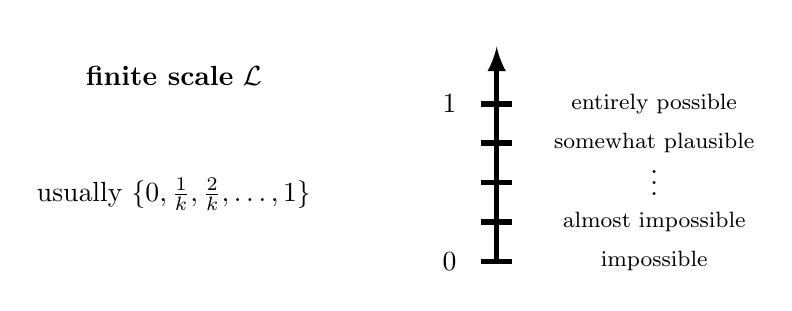
\begin{tikzpicture}
\node (top) at (1,2.5) {};
\node (bot) at (1,-0.5) {};
\draw[->,>=latex,line width=2pt] (bot) -- (top);
\node (finiteScale) at (-3.1,2) {\textbf{finite scale} $\mathcal{L}$};
\node (finiteScale2) at (-3.1,0.5) {usually $\{ 0, \frac{1}{k}, \frac{2}{k}, \ldots, 1 \}$};
\node at (0.4,1.65) {$1$};
\node at (3,1.65) {\footnotesize entirely possible};
\node at (3,1.15) {\footnotesize somewhat plausible};
\node at (3,0.75) {\vdots};
\node at (3,0.15) {\footnotesize almost impossible};
\node at (3,-0.35) {\footnotesize impossible};
\node at (0.4,-0.35) {$0$};
\draw[line width=2pt] (1.2,-0.35) -- (0.8,-0.35);
\draw[line width=2pt] (1.2,0.15) -- (0.8,0.15);
\draw[line width=2pt] (1.2,0.65) -- (0.8,0.65);
\draw[line width=2pt] (1.2,1.15) -- (0.8,1.15);
\draw[line width=2pt] (1.2,1.65) -- (0.8,1.65);
\end{tikzpicture}
%$1 = l_1 > l_2 > \ldots > l_{\# \mathcal{L}} = 0$ form the 
\begin{exampleblock}{}	
\flushleft events $e \subset \Omega$ (universe) \\ 
\centering
\textbf{sorted} using possibility \textbf{degrees} $\pi(e) \in \mathcal{L}$ \\
	$\neq$ \\
	\textbf{quantified} with \textbf{frequencies} $\textbf{p}(e) \in \croch{0,1}$ (probabilities)
	\end{exampleblock}
\visible<2->{
	\begin{block}{}
	$e_1 \neq e_2$, $2$ events $\subset \Omega$ 
	\begin{itemize}
	\item $ \pi(e_1) < \pi(e_2) $ $\Leftrightarrow$ \textit{``$e_1$ 
is less plausible than $e_2$''} \\
	\end{itemize}	
	\end{block}
}
\end{frame}




\begin{frame}
\frametitle{Qualitative Possibility Theory}
\framesubtitle{\footnotesize Criteria from Sugeno integral}
	\begin{alertblock}{}
	\centering
	{\hspace{-2.2cm} \color{red} Probability \hspace{0.3cm} / \hspace{0.1cm} Possibility}: \hspace{2cm}
	\begin{tabular}{!{\vrule width 2pt}c!{\vrule width 1pt}c!{\vrule width 2pt}c!}
	\noalign{\hrule height 2pt} 
 	 $ + $  & $ \max $ \\
	\noalign{\hrule height 2pt}  	
	 $ \times $  & $\min $ \\
	\noalign{\hrule height 2pt} 
	 $ X \in \mathbb{R} $  & $ X \in \mathcal{L} $ \\
	\noalign{\hrule height 2pt} 
									  	& \textbf{optimistic:}\\
										& \\
									 	& $ \displaystyle \mathbb{S}_{\Pi}[X] = \max_{x \in X} \min \set{ x, \pi(x) } $ \\
	$\displaystyle \mathbb{E}[X] = \sum_{x \in X} x \cdot \textbf{p}(x) $	& \\
										& \\
										& \textbf{pessimistic:} \\
										& \\
										& $ \displaystyle \mathbb{S}_{\mathcal{N}}[X] = \min_{x \in X} \max \set{ x, 1  - \pi(x) } $ \\

	\noalign{\hrule height 2pt}  	
	\end{tabular}
	\end{alertblock}
\end{frame}

\begin{frame}
\definecolor{bblue}{rgb}{0,0.4,0.75}
	\frametitle{Qualitative Possibility Theory}
	\framesubtitle{\footnotesize qualitative possibilistic POMDP ($\pi$-POMDP)}
\center 
\textit{Sabbadin (UAI-98)} introduces\\ 
\begin{alertblock}{\center the qualitative possibilistic POMDP}
\center \textbf{$\pi$-POMDP:} $\langle \mathcal{S}, \mathcal{A}, \mathcal{O}, T^{\pi}, O^{\pi}, \rho \rangle$
\end{alertblock}
\visible<2->{
\begin{itemize}
\item \textbf{transition} function $T^{\pi}(s,a,s') = \pi \paren{ s' \sachant s, a } \in \mathcal{L}$
\item \textbf{observation} function $O^{\pi}(s',a,o') = \pi \paren{ o' \sachant s', a } \in \mathcal{L}$
\item \textbf{preference} function $\rho: \mathcal{S} \times \mathcal{A} \rightarrow \mathcal{L}$
\end{itemize}
}
\visible<3->{
\begin{exampleblock}{}
\begin{itemize}
\item belief space trick: POMDP $\rightarrow$ MDP with \textbf{infinite} space\\% $\mathcal{S}$\\ 
\hspace{2.7cm} $\pi$-POMDP $\rightarrow$ $\pi$-MDP with \textbf{finite} space %$\mathcal{S}$
\item problem becomes \textbf{decidable}
\item $\forall s \in \mathcal{S}$, $\pi(s) = 1$ $\Leftrightarrow$ total ignorance about $s$
\end{itemize}
\end{exampleblock}
}
%\visible<3->{
%possibilistic POMDPs ($\pi$-POMDPs): \textit{Sabbadin UAI-98}.
%\begin{itemize}
%\item finite belief space \color{red} $\# \mathcal{B} = \# \mathcal{L}^{\# \mathcal{S}} - (\# \mathcal{L}-1)^{\# \mathcal{S}}$ \color{black} 
%\end{itemize}
%}
\end{frame}

\begin{frame}
\definecolor{bblue}{rgb}{0,0.4,0.75}
\frametitle{A possibilistic belief state}
\framesubtitle{\footnotesize finite belief space}
\vspace{0.4cm}
$\Pi^{\mathcal{S}}_{\mathcal{L}} = \Big\{$ possibility distributions $\Big\}$: $\# \Pi^{\mathcal{S}}_{\mathcal{L}} \sim \# \mathcal{L}^{\# \mathcal{S}} < + \infty$\\ 
\vspace{0.1cm} 
$\rightarrow $ \textit{i.e.} \textbf{finite belief space}
\vspace{-0.1cm}
\visible<2->{
\[ { \color{bblue}  b^{\pi}_{t} (s) = \pi \paren{ s_t = s \sachant a_0,o_1, \ldots, a_{t-1}, o_t } } \]
}
\vspace{-0.6cm}
\visible<3->{
\begin{exampleblock}{\textbf{possibilistic} belief update -- $a$ selected, $o'$ received}
\vspace{0.1cm}
joint distribution on $\mathcal{S} \times \mathcal{O}$ from $b_t^{\pi}$: $\pi \paren{ o', s' \sachant b_t^{\pi}, a}$ \\
\vspace{0.3cm}
\visible<4->{
$\rightarrow$ \textbf{next belief state:} $b^{\pi}_{t+1}(s') = \pi \paren{ o', s' \sachant b_t^{\pi}, a}$ \\
unless $s'$ maximizes $\pi \paren{ o', s' \sachant b_t^{\pi}, a}$, then $b^{\pi}_{t+1}(s') = 1$
\vspace{0.3cm}
% \left \{ \begin{array}{ccc} 1 & \hspace{-1cm} \mbox{ if } \pi \paren{ o',s' \sachant b_t^{\pi}, a} = \pi \paren{ o' \sachant b_t^{\pi}, a} \\
%\pi \paren{ o', s' \sachant b_t^{\pi}, a} & \mbox{ otherwise}  
%\end{array} \right.$ \\
\vspace{0.3cm}
${ \color{red} \mbox{ denoted by } }  { b^{\pi}_{t+1}(s') \color{red} \propto^{\pi} \pi \paren{o',s'\sachant b_t^{\pi}, a}} $
}
\end{exampleblock}
}
%\visible<4>{
%\begin{itemize}
%\item $\displaystyle  \pi ( o', s' \vert b_t^{\pi}, a)  = \max_{s \in \mathcal{S}} \min \Big\{ \pi ( o' \vert s', a ), \pi ( s' \vert s, a ), b^{\pi}_t(s) \Big\}$;
%\item $ \displaystyle \pi \paren{o' \sachant s', a} = \max_{s' \in \mathcal{S} } \pi \paren{ o',s' \sachant b^{\pi}_t, a  }$.
%\end{itemize}
%}
\vspace{-0.2cm}
\visible<5->{
\begin{block}{}
\begin{itemize}
\item \textbf{Makovian update:} only depends on $o'$, $a$ and $b_t^{\pi}$
\end{itemize}
\end{block}
}
\end{frame}




\begin{frame}
\frametitle{Overview}
\begin{block}{}
\textbf{Qualitative Possibility Theory:}\\ 
$\rightarrow$ simplification, imprecision/prior ignorance modeling
\end{block}
\vspace{1cm}
\visible<2->{
\begin{enumerate}
\item example of a qualitative possibilistic model
\item advancements and first use of the $\pi$-POMDP model 
\item simplify computation: ADDs and factorization 
\item probabilistic-possibilistic (hybrid) approach
\end{enumerate}
}
\end{frame}





}
%%%%%%%%%%%%%%%%%%%%%%%%%%%%%%%%%%%%%%%%%%%%%%%%%%
%%%%%%%%%%%%%%%%%%%%%%%%%%%%%%%%%%%%%%%%%%%%%%%%%%
%%%%%%%%%%%%%%%%%%%%%%%%%%%%%%%%%%%%%%%%%%%%%%%%%%
%%%%%%%%%%%%%%%%%%%%%%%%%%%%%%%%%%%%%%%%%%%%%%%%%%
%%%%%%%%%%%%%%%%%%%%%%%%%%%%%%%%%%%%%%%%%%%%%%%%%%
%%%%%%%%%%%%%%%%%%%%%%%%%%%%%%%%%%%%%%%%%%%%%%%%%%
%%%%%%%%%%%%%%%%%%%%%%%%%%%%%%%%%%%%%%%%%%%%%%%%%%
%%%%%%%%%%%%%%%%%%%%%%%%%%%%%%%%%%%%%%%%%%%%%%%%%%
%%%%%%%%%%%%%%%%%%%%%%%%%%%%%%%%%%%%%%%%%%%%%%%%%%
%%%%%%%%%%%%%%%%%%%%%%%%%%%%%%%%%%%%%%%%%%%%%%%%%%
%%%%%%%%%%%%%%%%%%%%%%%%%%%%%%%%%%%%%%%%%%%%%%%%%%
%%%%%%%%%%%%%%%%%%%%%%%%%%%%%%%%%%%%%%%%%%%%%%%%%%
%%%%%%%%%%%%%%%%%%%%%%%%%%%%%%%%%%%%%%%%%%%%%%%%%%
%%%%%%%%%%%%%%%%%%%%%%%%%%%%%%%%%%%%%%%%%%%%%%%%%%
%%%%%%%%%%%%%%%%%%%%%%%%%%%%%%%%%%%%%%%%%%%%%%%%%%

%%%%%%%%%%%%%%%%%%%%%%%%%%%%%%%%%%%%%%%%%%%%%%%%%%
%%%%%%%%%%%%%%%%%%%%%%%%%%%%%%%%%%%%%%%%%%%%%%%%%%
%%%%%%%%%%%%%%%%%%%%%%%%%%%%%%%%%%%%%%%%%%%%%%%%%%
%%%%%%%%%%%%%%%%%%%%%%%%%%%%%%%%%%%%%%%%%%%%%%%%%%
%%%%%%%%%%%%%%%%%%%%%%%%%%%%%%%%%%%%%%%%%%%%%%%%%%
%%%%%%%%%%%%%%%%%%%%%%%%%%%%%%%%%%%%%%%%%%%%%%%%%%
%%%%%%%%%%%%%%%%%%%%%%%%%%%%%%%%%%%%%%%%%%%%%%%%%%
%%%%%%%%%%%%%%%%%%%%%%%%%%%%%%%%%%%%%%%%%%%%%%%%%%
%%%%%%%%%%%%%%%%%%%%%%%%%%%%%%%%%%%%%%%%%%%%%%%%%%
%%%%%%%%%%%%%%%%%%%%%%%%%%%%%%%%%%%%%%%%%%%%%%%%%%
%%%%%%%%%%%%%%%%%%%%%%%%%%%%%%%%%%%%%%%%%%%%%%%%%%
%%%%%%%%%%%%%%%%%%%%%%%%%%%%%%%%%%%%%%%%%%%%%%%%%%
%%%%%%%%%%%%%%%%%%%%%%%%%%%%%%%%%%%%%%%%%%%%%%%%%%
%%%%%%%%%%%%%%%%%%%%%%%%%%%%%%%%%%%%%%%%%%%%%%%%%%
%%%%%%%%%%%%%%%%%%%%%%%%%%%%%%%%%%%%%%%%%%%%%%%%%%




\section[qualitative modeling]{Introductory example (HMI)}

\begin{frame}
\frametitle{Example: Human-Machine Interaction (HMI)}
\framesubtitle{\footnotesize joint work with \textbf{Sergio Pizziol} -- Context}
\vspace{0.1cm}
\begin{figure}
\centering
\begin{tikzpicture}[scale=1,transform shape]
%states
\tikzstyle{vertex}=[fill=black!20,draw=black,  minimum width=85pt,line width=1pt,inner sep=5pt, minimum height=60pt]
\tikzstyle{vertexBIG}=[fill=black!20,draw=black, minimum width=280pt, minimum height=40pt,line width=1pt,inner sep=5pt]

%% HMI
\node[vertex] (M) at (-1.5,-0.25) {};
\node () at (-1.1,0.5) {\textbf{Machine}};
\node[vertex] (H) at (5.5,-0.25) {};
\node () at (4.95,0.5) {\textbf{Human}};
\node () at (5.8,-0.47) {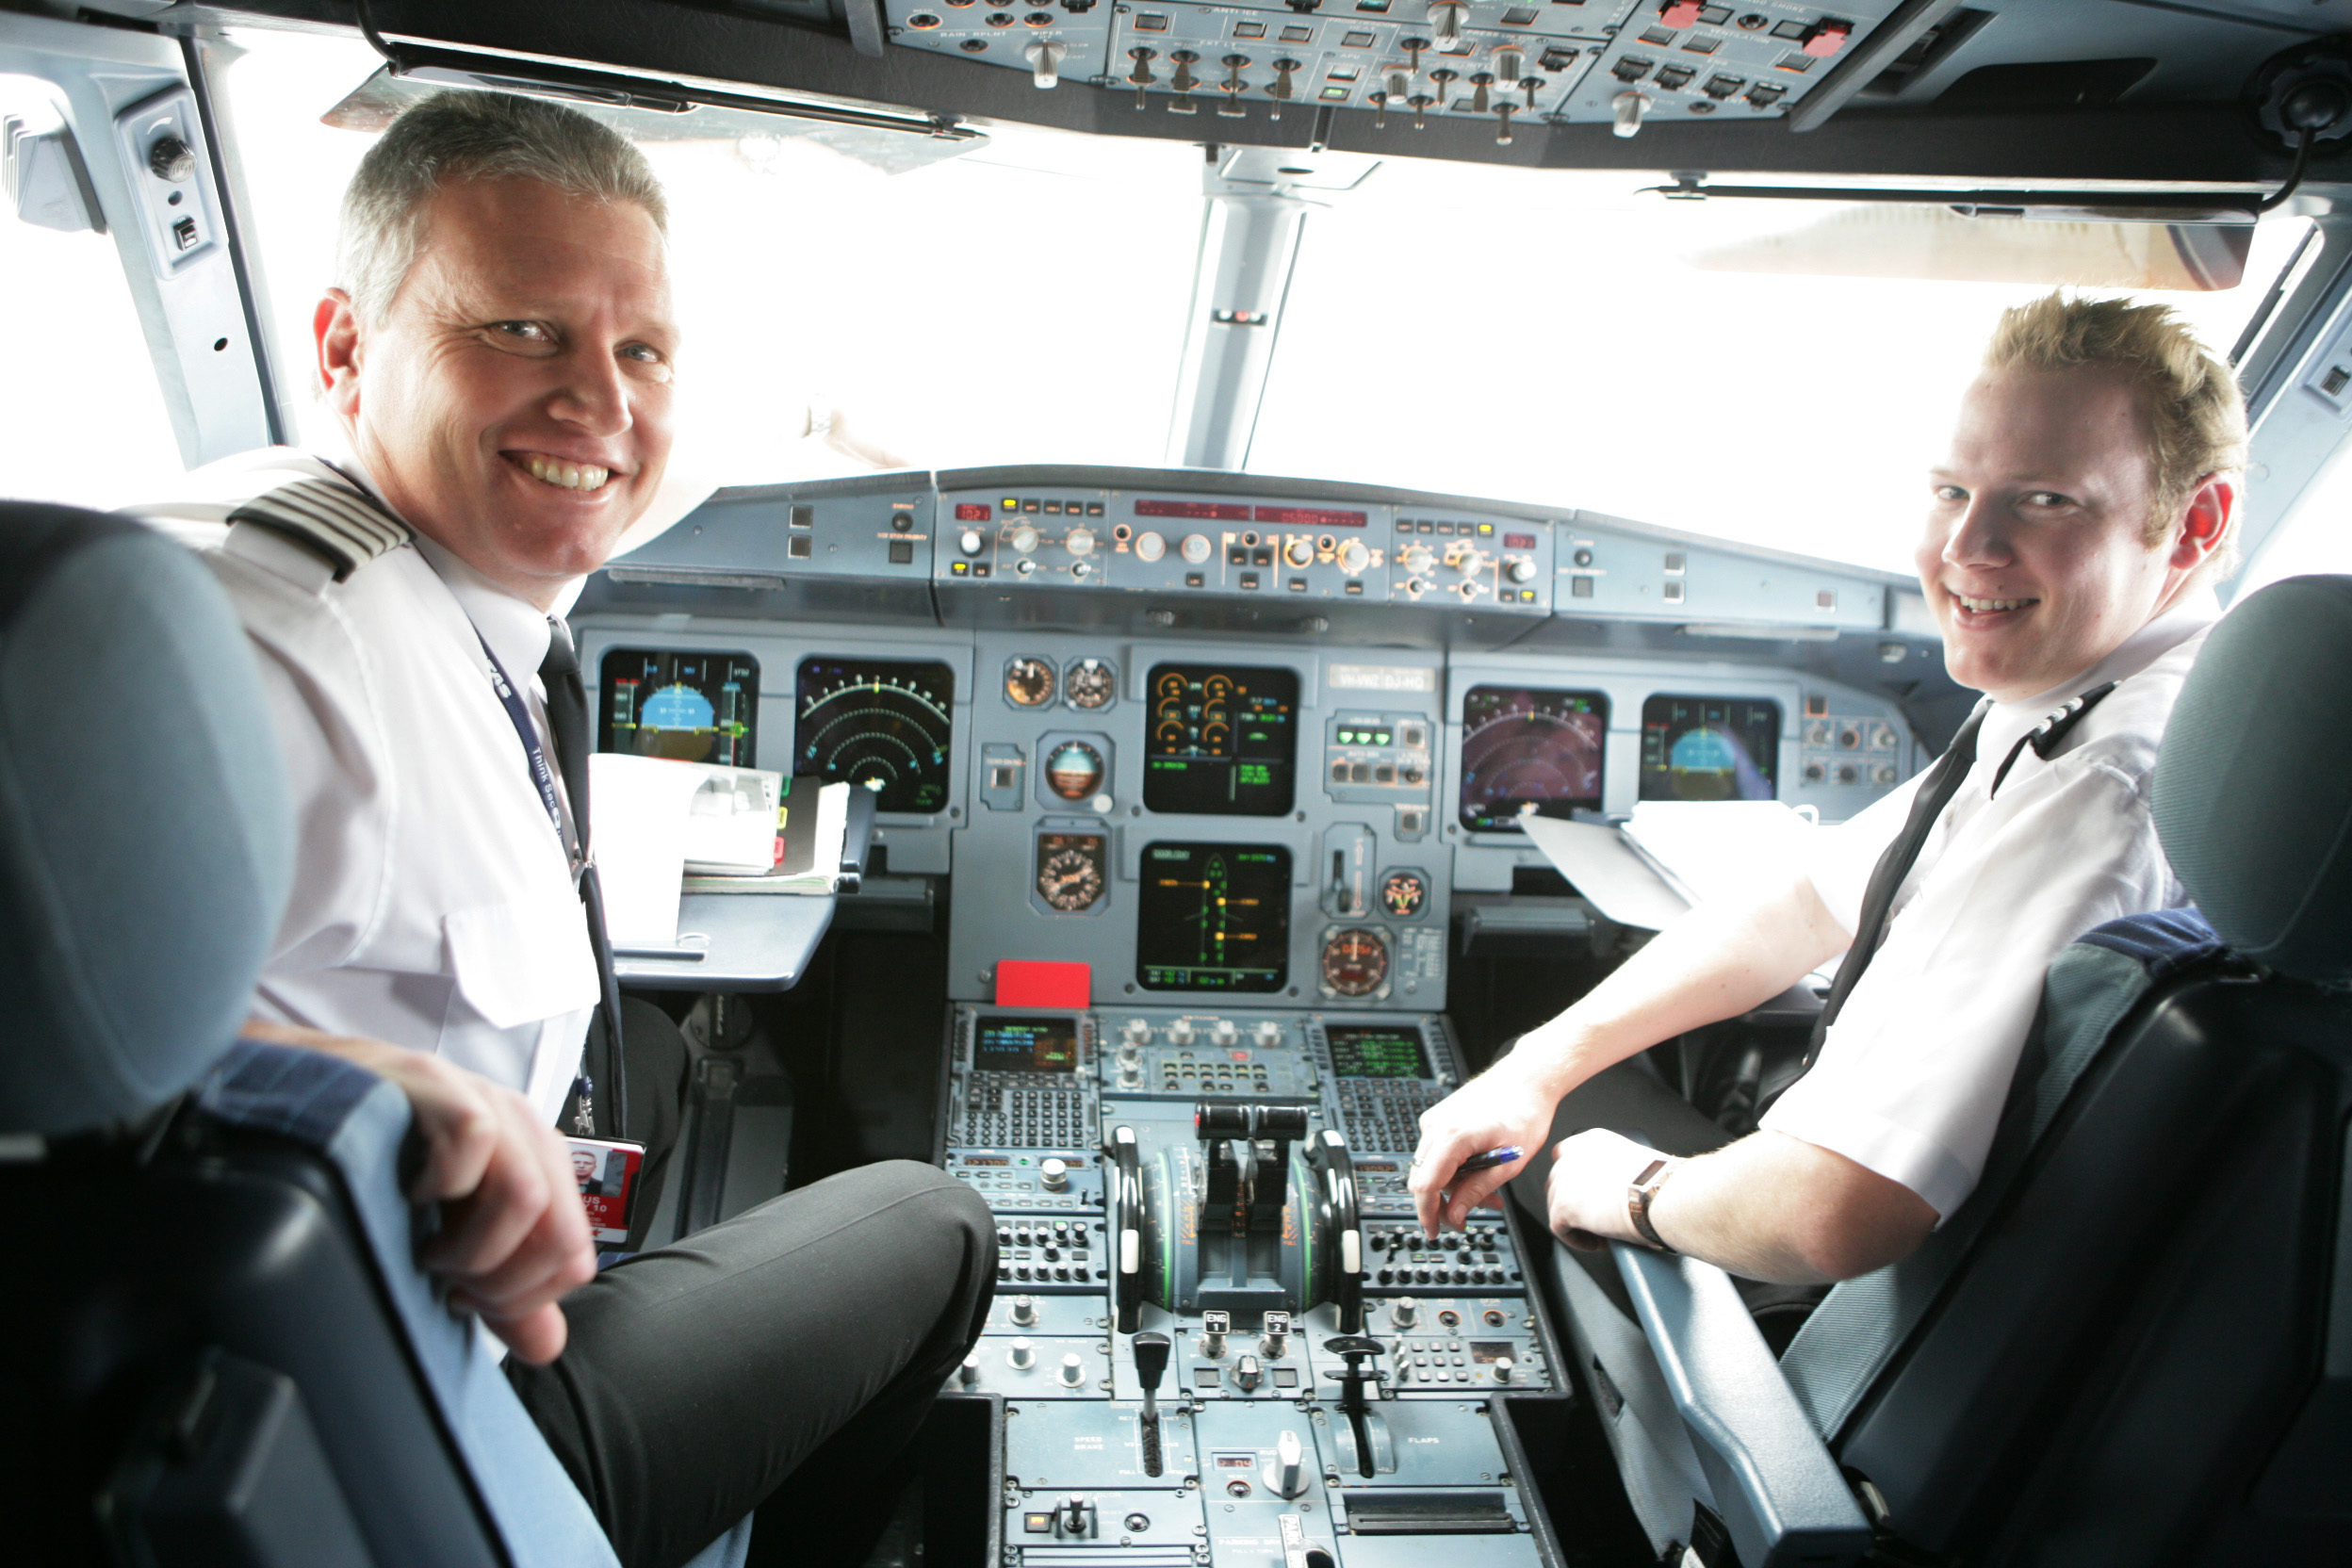
\includegraphics[scale=0.025]{6767906077_3f50cecffb_o}};
\node () at (-1,-0.6) {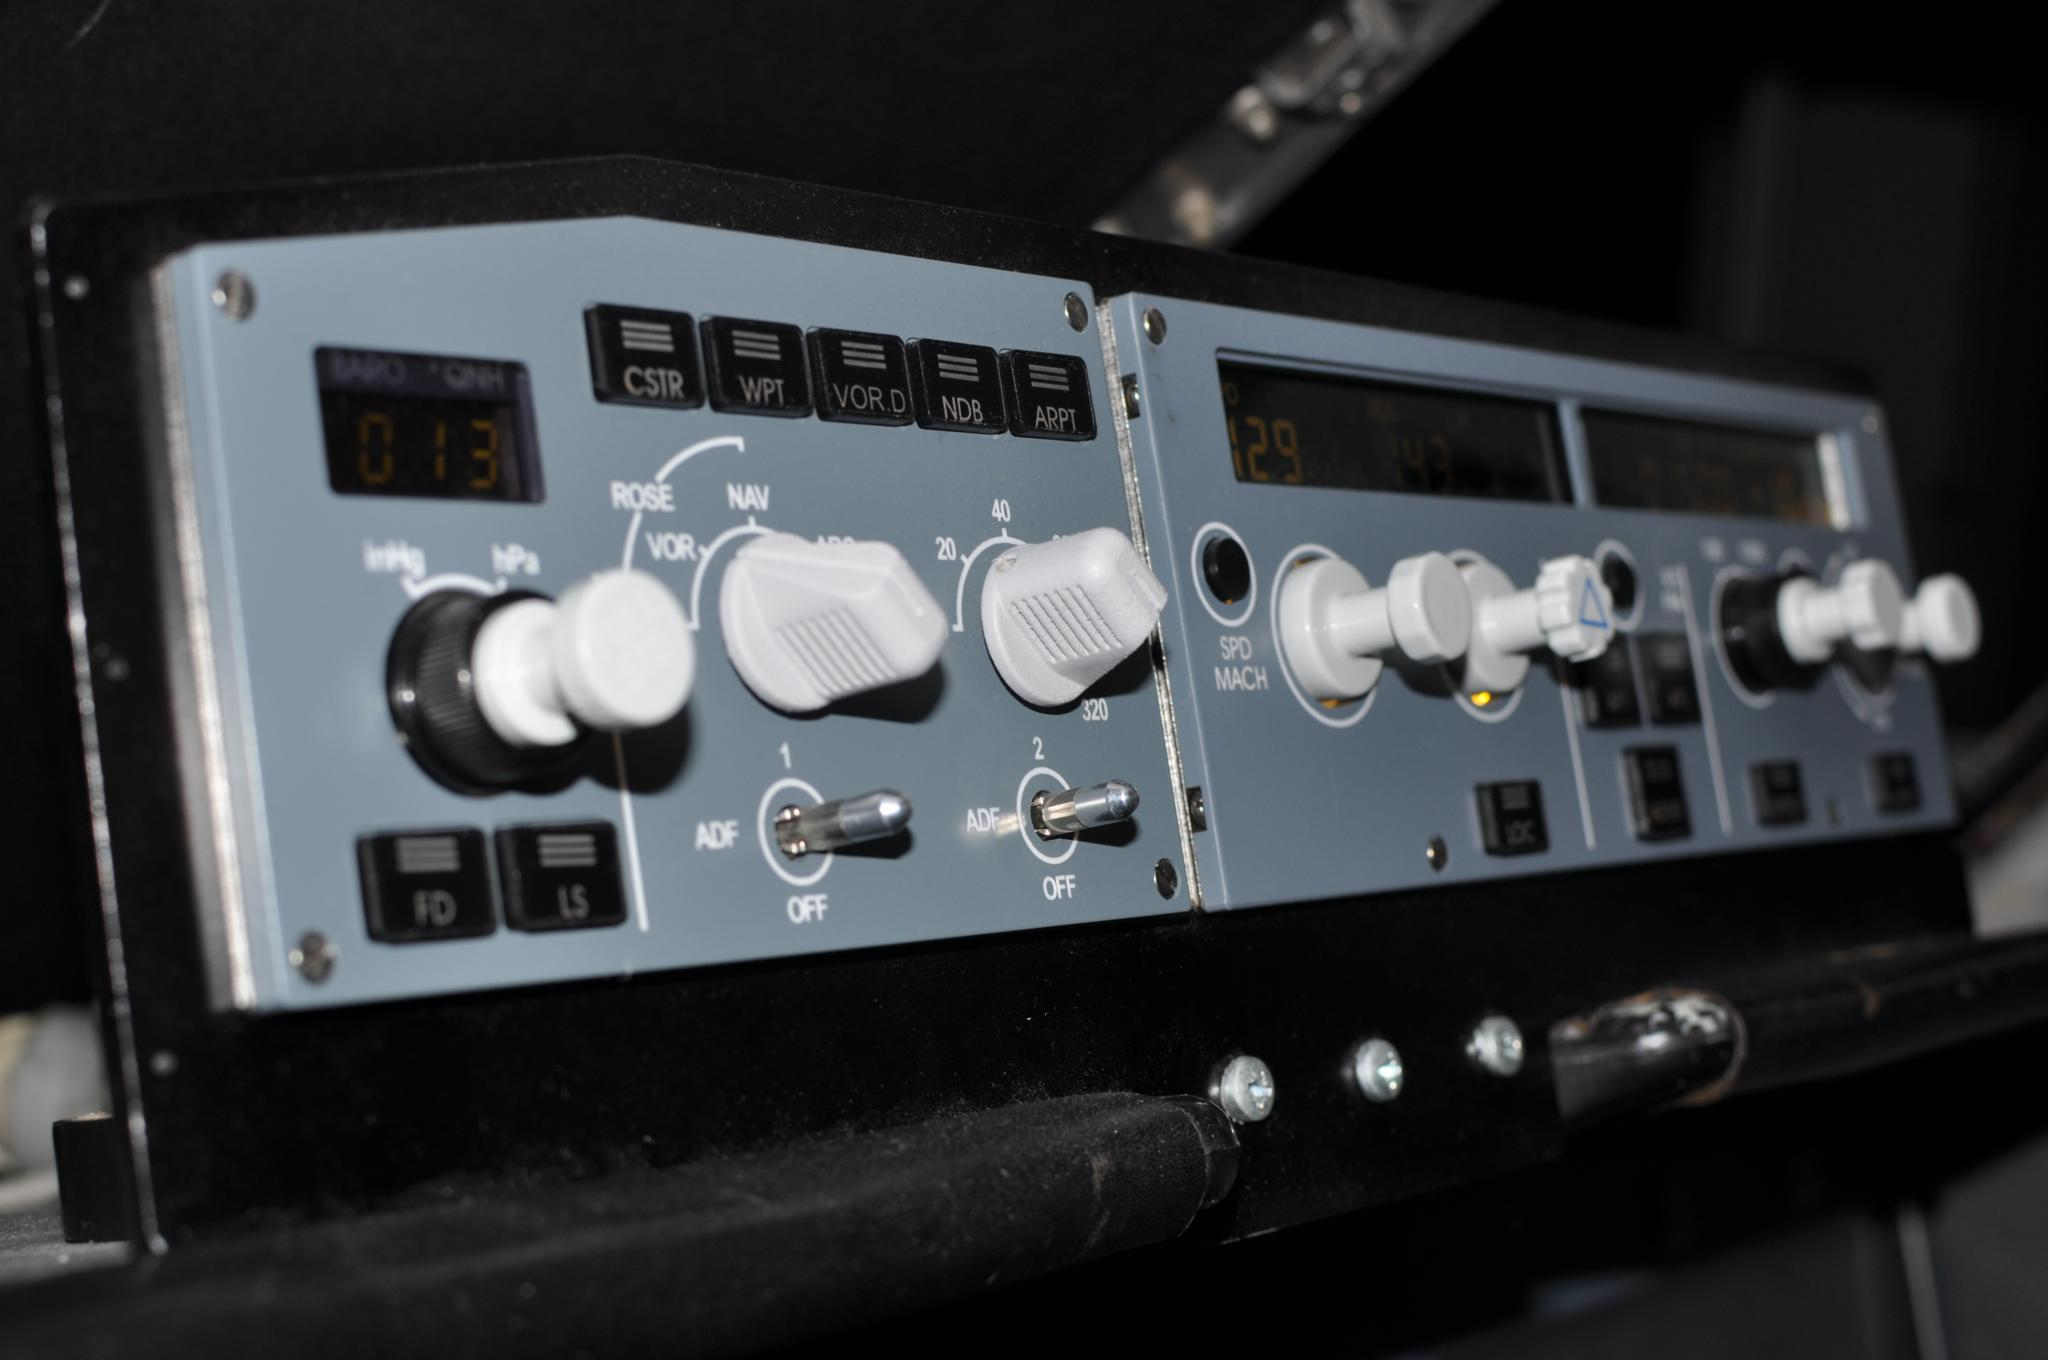
\includegraphics[scale=0.025]{fcu}};
\node () at (-2.45,-0.4) {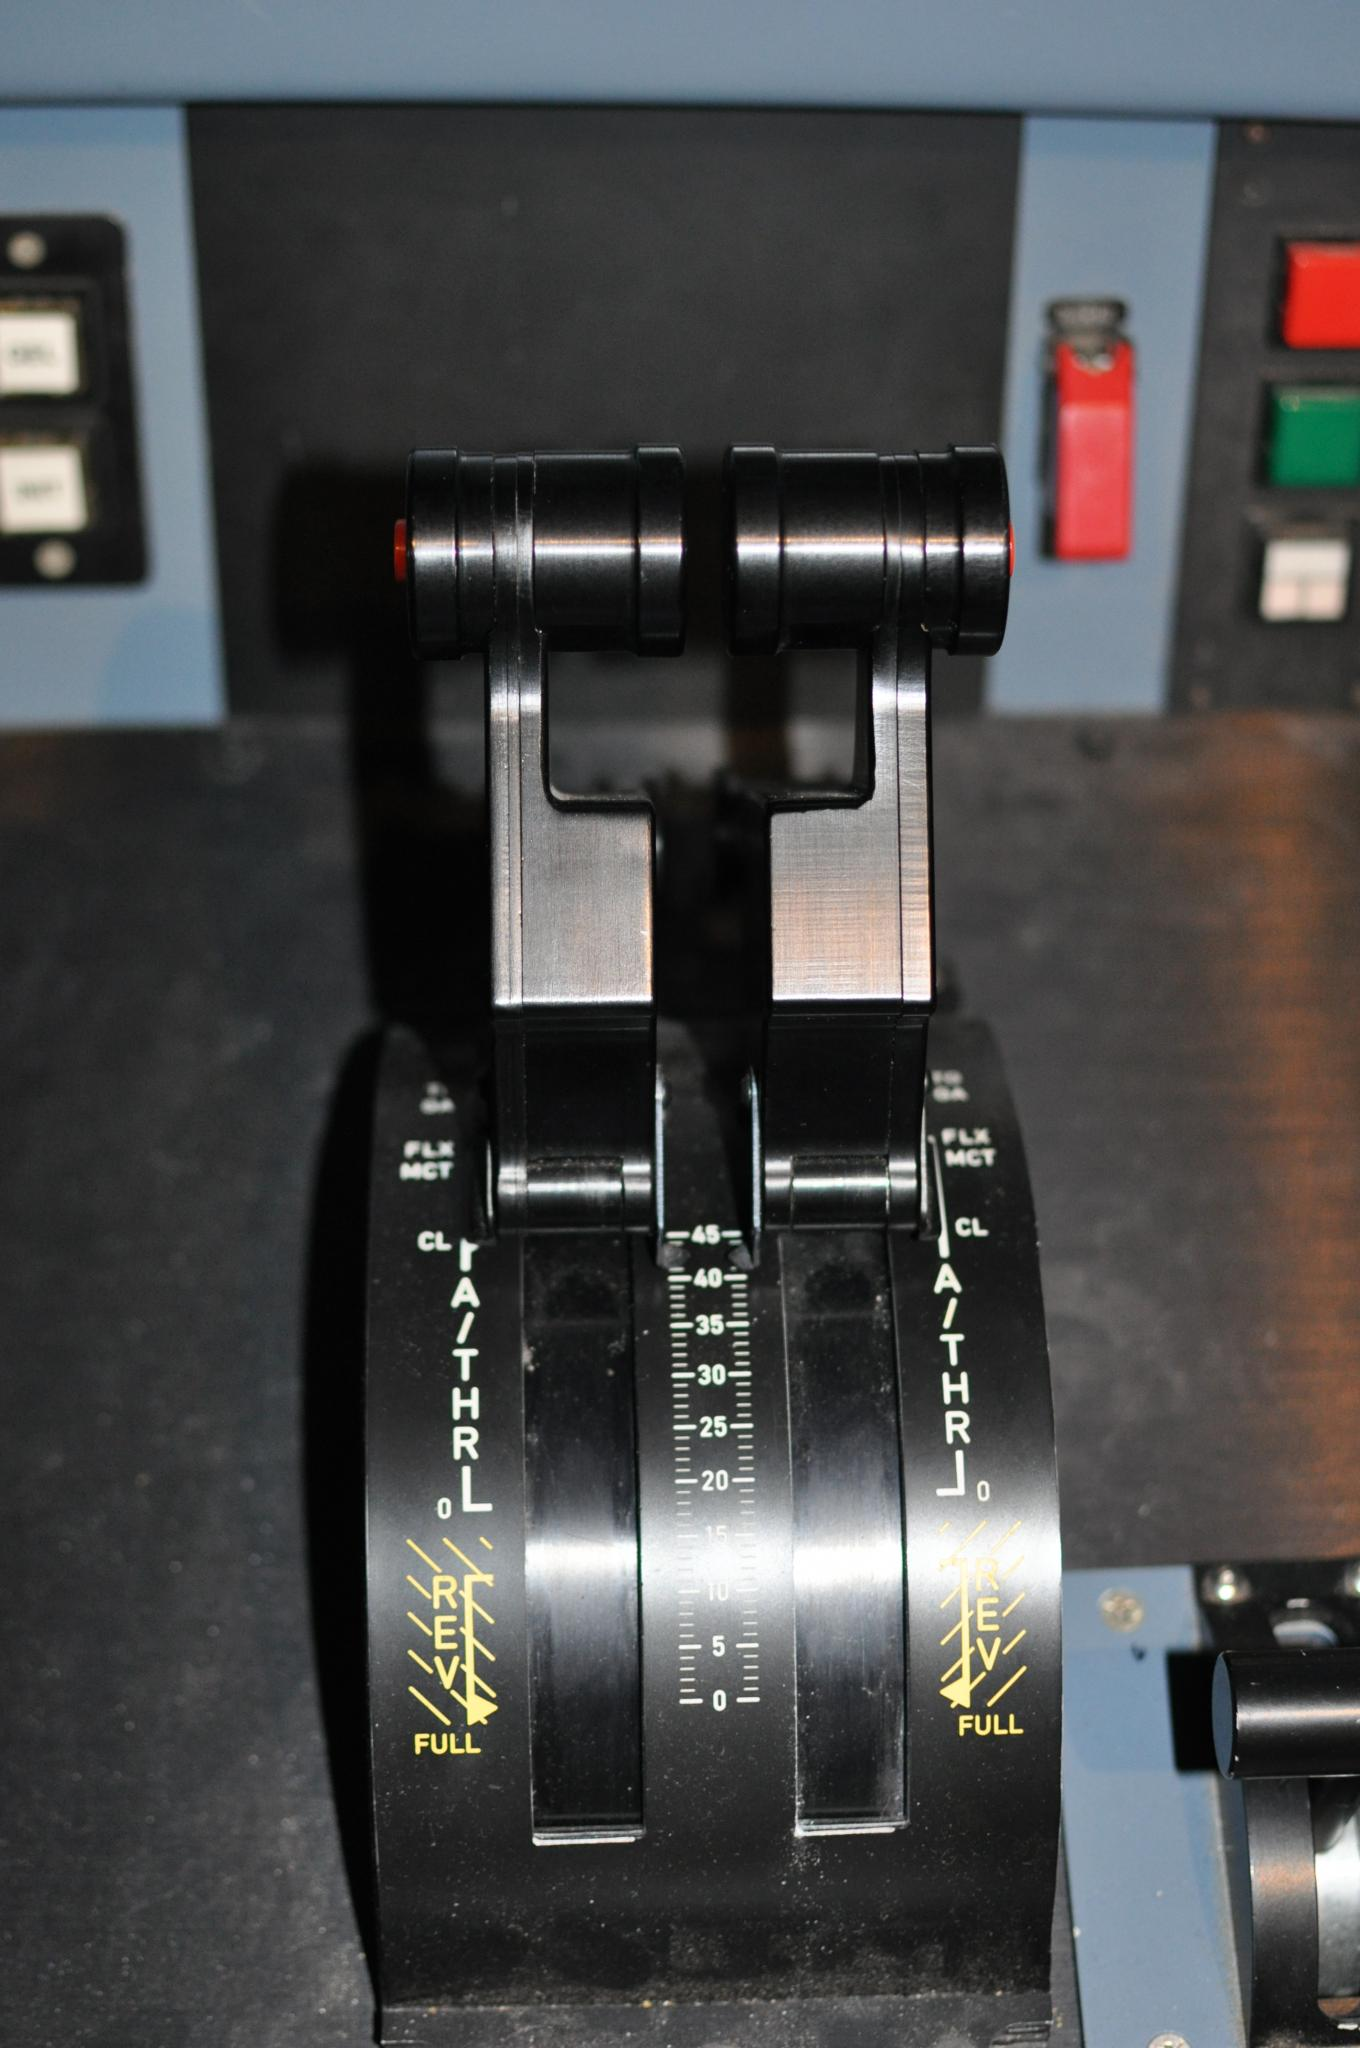
\includegraphics[scale=0.02]{manettegaz}};
%% ARROWS
\draw[->,>=latex,line width=4pt,color=red] (-0.15,0.3) -- (4.2,0.3);
\draw[->,>=latex,line width=4pt,color=red] (4.2,-1) -- (-0.15,-1);
%%LEGEND
\node () at (1,0.6) {\footnotesize Feedbacks};
\node () at (3,-0.4) {\footnotesize Interface};
\node () at (2.8,-0.75) {\footnotesize manipulations};

\visible<3->{
%% OBSERVER
\node[vertexBIG] (O) at (2,-2.5) {};
\node () at (1.9,-2.1) {\textbf{Observer}};
\node[ellipse,draw, thick,fill=blue!20] (el) at (-0.55,-2.7) {Machine model};
\node[ellipse,draw, thick,fill=blue!20] (el) at (4.15,-2.7) {Human error model};

\draw[->,>=latex,line width=2pt,color=red, dashed] (3,-1) -- (3,-2);
\draw[->,>=latex,line width=2pt,color=red, dashed] (0.8,0.3) -- (0.8,-2);
}

\end{tikzpicture}
%\caption{ 3 actors involved: red arrows = information flows.}
\end{figure}
\vspace{-0.3cm}
\visible<2->{
\begin{block}{}
\textbf{Issue:} incorrect human assessment of the machine state \\ 
\hspace{2cm} $\rightarrow$ \textbf{accident risk}
\end{block}
}
\vspace{-0.15cm}
\visible<4->{
\begin{alertblock}{$\pi$-POMDP without actions: $\pi$-Hidden Markov Process}
\begin{itemize}
\item \textbf{system space} $\mathcal{S}$: set of human assessments $\rightarrow$ \textbf{hidden} 
\item \textbf{observation space} $\mathcal{O}$: feedbacks/human manipulations
\end{itemize}
\end{alertblock}
}
\end{frame}





\begin{frame}
\frametitle{Example: Human-Machine Interaction (HMI)}
\framesubtitle{\footnotesize Human error model from expert knowledge}
\vspace{0.2cm}
\begin{alertblock}{Machine with states $A$, $B$, $C$, $\ldots$}
state $s_A \in \mathcal{S}$: ``human thinks machine state is $A$'' 
\end{alertblock}
\visible<2->{
	\begin{exampleblock}{ Machine state transition $A \rightarrow B$}
	\begin{itemize}
		\item observation: \textbf{machine feedback} $o_f' \in \mathcal{O}$: 
	\end{itemize}
	\textit{``human usually aware of feedbacks''} $\rightarrow$ $\pi \paren{s_B',o_f' \sachant s_A} = 1$\\
	\hspace{1.5cm} \textit{``but may lose a feedback''} $\rightarrow$ $\pi \paren{s_A',o_f' \sachant s_A} = \frac{2}{3}$ 
	\visible<3->{
		\begin{itemize}
			\item  observation: \textbf{human manipulation} $o_m' \in \mathcal{O}$:
		\end{itemize}
		\textit{``manipulation $o_m'$ is normal under $s_A$''} $\rightarrow$ $\pi \paren{s_B',o_m' \sachant s_A} = 1$\\
		\hspace{2.8cm} \textit{``is abnormal''} \hspace{1.1cm} $\rightarrow $ \hspace{2cm} $ = \frac{1}{3}$ 
	}
	\visible<4->{
		\begin{itemize}
			\item impossible cases: possibility degree $0$
		\end{itemize}
	}
	\end{exampleblock}
}
\end{frame}



\begin{frame}
\frametitle{Qualitative Possibilistic Hidden Markov Process:}
\framesubtitle{\footnotesize $\pi$-HMP, detection $\&$ diagnosis tool for HMI (with \textbf{Sergio Pizziol})}
\vspace{0.3cm}
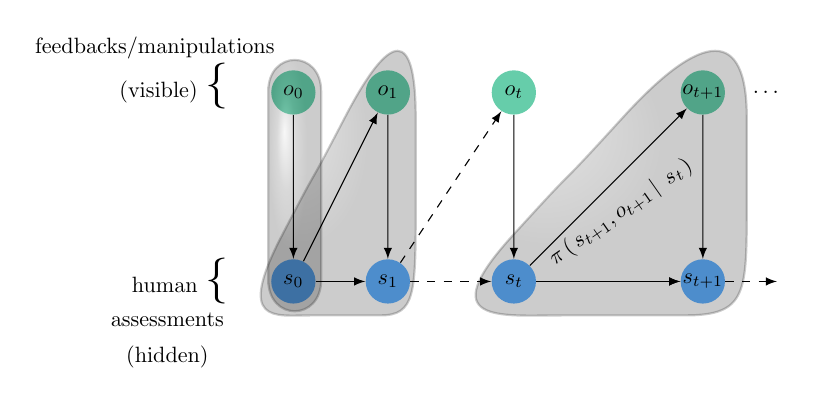
\begin{tikzpicture}[scale=0.8,transform shape]

%TIME
%\node [font=\huge] (statet) at (3.8,1) {$t$};
%\node [font=\huge] (statetplus1) at (8.9,1) {$t+1$};
%%%%%%%%%%%%%%%%%%%%%%%%%%%%%%%%%%%%%%%%%%%%%%%%%%%%%%%%%%%%%%%%%%%%%%%%
%states
\tikzstyle{vertex}=[circle,fill=DodgerBlue!70,minimum size=20pt,inner sep=0pt]
\tikzstyle{mvertex}=[circle,fill=DodgerBlue!70,minimum size=30pt,inner sep=0pt]
\tikzstyle{overtex}=[circle,fill=MediumAquamarine,minimum size=20pt,inner sep=0pt]


\node (Oc) at (0.8,3.7) {feedbacks/manipulations};
\node (V) at (1.1,3.1) {(visible) \huge $\{$};
%\node (V) at (1.5,1) {effects \huge $\{$};
\node (H) at (1.2,0) {human \huge $\{$};
\node (H1) at (1,-0.6) {assessments};
\node (H1) at (1,-1.2) {(hidden)};

%\node (E) at (1.7,1.5) {effects \huge $\{$};

%1
\node[overtex] (state1) at (3,3) {$o_0$};
%\node[vertex] (state11) at (2.5,1) {$e_0$};
\node[vertex] (state111) at (3,0) {$s_0$};
%2
\node[overtex] (state2) at (4.5,3) {$o_1$};
%\node[vertex] (state22) at (4,1) {$e_1$};
\node[vertex] (state222) at (4.5,0) {$s_1$};

\node[overtex] (state3) at (6.5,3) {$o_t$};
%\node[vertex] (state33) at (6,1) {$e_t$};
\node[vertex] (state333) at (6.5,0) {$s_t$};

\node (H) at (8.2,1.1) [rotate=35] {$\pi \paren{s_{t+1},o_{t+1} \sachant s_t}$};

\node[overtex] (state4) at (9.5,3) {$o_{t+1}$};
%\node[vertex] (state44) at (8,1) {$e_{t+1}$};
\node[vertex] (state444) at (9.5,0) {$s_{t+1}$};


\node (state23) at (10.5,3) {$\hdots$};

%3
\node (state5) at (10.8,2) {};
\node (state55) at (10.8,1) {};
\node (state555) at (10.8,0) {};

%\node (e0) at (2.9,1.6) [color=black!70] {\huge $e_0$};
%\node (e1) at (4.2,1.6) [color=black!70] {\huge $e_1$};
%\node (et) at (8.9,1.6) [color=black!70] {\huge $e_{t+1}$};

%SV
% arrows sv->sv
%1->2
\draw[->,>=latex] (state1) -- (state111);
\draw[->,>=latex] (state111) -- (state2);
\draw[->,>=latex] (state111) -- (state222);
%\draw[->,>=latex] (state111) -- (state11);
%\draw[->,>=latex] (state1) -- (state11);


\draw[->,>=latex] (state2) -- (state222);
\draw[->,>=latex,dashed] (state222) -- (state3);
\draw[->,>=latex,dashed] (state222) -- (state333);
%\draw[->,>=latex] (state2) -- (state22);
%\draw[->,>=latex] (state222) -- (state22);
%\draw[->,>=latex] (state111) -- (state22);

\draw[->,>=latex] (state3) -- (state333);
\draw[->,>=latex] (state333) -- (state444);
\draw[->,>=latex] (state333) -- (state4);

%\draw[->,>=latex] (state333) -- (state33);
%\draw[->,>=latex] (state3) -- (state33);
%\draw[->,>=latex,dashed] (state222) -- (state33);
\draw[->,>=latex] (state333) -- (state444);
\draw[->,>=latex] (state4) -- (state444);
\draw[->,>=latex,dashed] (state444) -- (state555);

%\draw[->,>=latex] (state444) -- (state44);
%\draw[->,>=latex] (state4) -- (state44);
%\draw[->,>=latex] (state333) -- (state44);

\draw [scale=0.7,xscale=1.4,ball color=black,opacity=0.2,xshift=40,yshift=35,thick=5pt]
 (9,2.5)..controls +(0,2) and +(1.3,2) ..(7,2.5) % angle haut
 ..controls +(-1.3,-2) and +(1.3,2) ..(5.2,-0.2) % ligne gauche inclinee
 ..controls +(-1.3,-2) and +(-1,0).. (6,-2) % angle inferieur gauche
 ..controls +(-1,0) and +(1,0).. (8,-2)
 ..controls +(1,0) and +(0,-2).. (9,0.5) % angle inferieur droit
 ..controls +(0,1) and +(0,-1).. (9,2.5); % arc 4

\draw [scale=0.7,xscale=0.8,ball color=black,opacity=0.2,xshift=-5,yshift=35,thick=5pt]
 (9,2.5)..controls +(0,2) and +(1.3,2) ..(7,2.5) % angle haut
 ..controls +(-1.3,-2) and +(1.3,2) ..(5.2,-0.2) % ligne gauche inclinee
 ..controls +(-1.3,-2) and +(-1,0).. (6,-2) % angle inferieur gauche
 ..controls +(-1,0) and +(1,0).. (8,-2)
 ..controls +(1,0) and +(0,-2).. (9,0.5) % angle inferieur droit
 ..controls +(0,1) and +(0,-1).. (9,2.5); % arc 4


\draw [scale=0.7,xscale=0.8,yscale=0.95,ball color=black,opacity=0.2,xshift=-67,yshift=58,thick=5pt]
 (8.5,2.5)..controls +(0,1) and +(0,1) ..(7,2.5) % angle haut
 ..controls +(0,1) and +(0,-1) ..(7,-2) 
 ..controls +(0,-1) and +(0,-1).. (8.5,-2) % angle inferieur droit
 ..controls +(0,1) and +(0,-1).. (8.5,2.5); % arc 4

%%%%%%%%%%%%%%%%%%%%%%%%%%%%%%%%%%%%%%%%%%%%%%%%%%%%%%%%%%%%%%
% TRANSITION FUNCTIONS
%\node (T1) at (7.1,2.05) {$T^{a,1}$};
%\node (T2) at (7,1.45) {$T^{a,2}$};
\end{tikzpicture}
\visible<2->{
\begin{itemize}
\item \textbf{estimation} of the human assessment\\
\hspace{3cm}$\Leftrightarrow$ \textbf{possibilistic belief state}% over $s \in \mathcal{S}$ 
\item \textbf{detection} of human assessment errors + \textbf{diagnosis}
\item validated with pilots on flight simulator missions
\end{itemize}
}
\end{frame}

\section[advances in $\pi$-POMDP]{Advances in the qualitative possibilistic MDPs}%Mixed-Observability and unbounded mission durations}
\begin{frame}
\frametitle{Applicability of the $\pi$-POMDPs}
\framesubtitle{\footnotesize three advancements}
\vspace{0.2cm}
\begin{itemize}
\item<alert@+> lack of proof of optimality in indefinite horizon settings
\item criterion/algorithm/proof
\end{itemize}
\vspace{0.4cm}
\begin{itemize}
\item<alert@+> curse of dimensionality: \\
$\rightarrow$ belief space size of a $\pi$-POMDP:  exponential in $\# \mathcal{S}$\\
\item in practice, part of $s \in \mathcal{S}$ is visible\\
\hspace{4cm} $\Rightarrow$ complexity reduction  
\end{itemize}
\vspace{0.4cm}
\begin{itemize}
\item<alert@+> lack of possibilistic strategy evaluation
\item demonstration of usefulness\\ 
when probabilities are imprecise 
\end{itemize}


\visible<4->{
\begin{alertblock}{}
\begin{center}
\textbf{Indefinite Horizon, Mixed-Observability, Simulations}
\hspace{4cm} \textit{contribution UAI 2013}
\end{center}
\end{alertblock}
}


\end{frame}






\begin{frame}
\frametitle{Indefinite Horizon}
\framesubtitle{\footnotesize criterion, DP scheme, optimal strategy}
\vspace{0.1cm}
\textbf{indefinite horizon criterion:} \\ 
\vspace{0.2cm}
maximizing
\[ \min_{t=0}^{\# \delta} \min \bigg\{ \pi \Big( s' \Big\vert s, \delta_t(s) \Big), \Psi(s) \bigg\} \]
with respect to the strategy $\delta: (t,s) \mapsto a_t \in \mathcal{A}$.
\vspace{0.5cm}
\visible<2->{
\begin{block}{Dynamic Programming scheme: $\#$ iterations $<\# \mathcal{S}$}
\begin{itemize}
\item assumption: $\exists$ artificial \textbf{``stay'' action}\\ 
as in classical planning/ $\gamma$ counterpart 
\item criterion \textbf{non decreasing} with iterations
\visible<3->{
\item action update for states increasing the criterion
\item \textbf{proof of optimality} of the resulting \textbf{stationary} strategy
}
\end{itemize}
\end{block}
}
\end{frame}







\begin{frame}
\frametitle{Mixed-Observability {\footnotesize (MOMDP, \textit{Ong et al., 2005}) }}
\framesubtitle{\footnotesize $\pi$-Mixed-Observable Markov Decision Process ($\pi$-MOMDP)}
\textbf{graphical model} of a $\pi$-MOMDP:
\vspace{-0.6cm}
\begin{figure}\centering
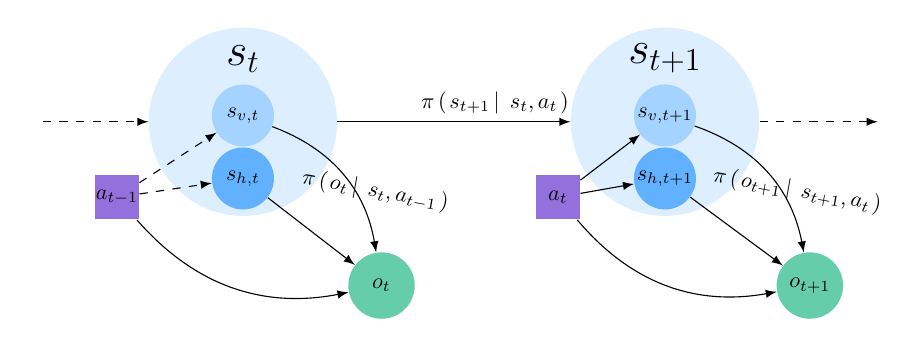
\begin{tikzpicture}[scale=0.8,transform shape]

%%%%%%%%%%%%%%%%%%%%%%%%%%%%%%%%%%%%%%%%%%%%%%%%%%%%%%%%%%%%%%%%%%%%%%%%
% macro states
\tikzstyle{mvertex}=[circle,fill=DodgerBlue!15,minimum size=85pt,inner sep=0pt]
\tikzstyle{overtex}=[circle,fill=MediumAquamarine,minimum size=30pt,inner sep=0pt]
\tikzstyle{avertex}=[fill=MediumPurple,minimum size=20pt,inner sep=0pt]

\tikzstyle{vertex}=[circle,fill=DodgerBlue!40,minimum size=28pt,inner sep=0pt]
\tikzstyle{hvertex}=[circle,fill=DodgerBlue!70,minimum size=28pt,inner sep=0pt]

%\tikzstyle{mvertex}=[circle,fill=black!15,minimum size=75pt,inner sep=0pt]
\node[mvertex] (state1) at (1.3,0) {};
\node [font=\huge] (state1t) at (1.3,1) {$s_t$};
\node[mvertex] (state2) at (8,0) {};
\node [font=\huge] (state2t) at (8,1) {$s_{t+1}$};
%0
\node (state0) at (-2,0) {};
%3
\node (state3) at (11.5,0) {};


%%%%%%%%%%%%%%%%%%%%%%%%%%%%%%%%%%%%%%%%%%%%%%%%%%%%%%%%%%%%%%%%%%%%%%%%
% possibilités
\node (pisasp) at (5.3,0.3) {$\pi \paren{ s_{t+1} \sachant s_{t},a_t }$};
\node (pisvshaoh1) at (3.4,-1.1) [rotate=350] {$\pi \paren{ o_{t} \sachant s_t,a_{t-1} }$};
\node (pisvshaoh2) at (10.1,-1.1) [rotate=350] {$\pi \paren{ o_{t+1} \sachant s_{t+1},a_{t} }$};

%%%%%%%%%%%%%%%%%%%%%%%%%%%%%%%%%%%%%%%%%%%%%%%%%%%%%%%%%%%%%%%%%%%%%%%%
%vstates
%\tikzstyle{vertex}=[circle,fill=black!30,minimum size=28pt,inner sep=0pt]
%1
\node[vertex] (vstate1) at (1.3,0.1) {$s_{v,t}$};
%2
\node[vertex] (vstate2) at (8,0.1) {$s_{v,t+1}$};
%\node [font=\huge] (state2t) at (8,0.9) {$s_{t+1}$};

%%%%%%%%%%%%%%%%%%%%%%%%%%%%%%%%%%%%%%%%%%%%%%%%%%%%%%%%%%%%%%%%%%%%%%%%
%hstates
%1
%\tikzstyle{hvertex}=[circle,fill=black!60,minimum size=28pt,inner sep=0pt]
\node[hvertex] (hstate1) at (1.3,-0.9) {$s_{h,t}$};
%2
\node[hvertex] (hstate2) at (8,-0.9) {$s_{h,t+1}$};


%%%%%%%%%%%%%%%%%%%%%%%%%%%%%%%%%%%%%%%%%%%%%%%%%%%%%%%%%%%%%%%%%%%%%%%%
%action
\node[avertex] (action) at (6.3,-1.2) {$a_t$};
\node[avertex] (action0) at (-0.7,-1.2) {$a_{t-1}$};

%%%%%%%%%%%%%%%%%%%%%%%%%%%%%%%%%%%%%%%%%%%%%%%%%%%%%%%%%%%%%%%%%%%%%%%%
% observations
%1
\node[overtex] (hobserv1) at (3.5,-2.6) {$o_{t}$};
%2
\node[overtex] (hobserv2) at (10.3,-2.6) {$o_{t+1}$};


%%%%%%%%%%%%%%%%%%%%%%%%%%%%%%%%%%%%%%%%%%%%%%%%%%%%%%%%%%%%%%
%ARROWS

%S
%0->1
\draw[->,>=latex,dashed] (state0) -- (state1);
%2->3
\draw[->,>=latex,dashed] (state2) -- (state3);
%1->2
\draw[->,>=latex] (state1) -- (state2);


%SV

% arrows sv->oh
%1
\draw[->,>=latex] (vstate1) to[bend left] (hobserv1);
%2
\draw[->,>=latex] (vstate2) to[bend left] (hobserv2);


%SH

% arrows sh->oh
%1
\draw[->,>=latex] (hstate1) to (hobserv1);
%2
\draw[->,>=latex] (hstate2) to (hobserv2);

%A
% a->s
%1
\draw[->,>=latex] (action) -- (vstate2);
\draw[->,>=latex] (action) -- (hstate2);
%0
\draw[->,>=latex,dashed] (action0) -- (vstate1);
\draw[->,>=latex,dashed] (action0) -- (hstate1);

% a->oh
%1
\draw[->,>=latex] (action) to[bend right]  (hobserv2);
%0
\draw[->,>=latex] (action0) to[bend right]  (hobserv1);

%\node (probao1) at (4,-2.2) [rotate=350] {$ \pi \paren{ o_{h,t} \sachant s_t, a_{t-1}}$};
%\node (probao2) at (11,-2.5) [rotate=350] {$ \pi \paren{ o_{h,t+1} \sachant s_{t+1}, a_{t}}$};
%\node (probas) at (8.9,0.5) [rotate=355] {$ \pi \paren{s_{t+1} \sachant s_t,a_{t}}$};
\end{tikzpicture}
\end{figure}
\vspace{-0.2cm}
\textbf{Mixed-Observability:} system state $s \in {\color{blue} \mathcal{S} = \mathcal{S}_v  \times \mathcal{S}_h} $ \\ 
\textit{i.e.} state $s \hspace{0.05cm} = \hspace{0.05cm} $ visible component $s_v$ \hspace{0.05cm} $\&$ \hspace{0.05cm} hidden component $s_h$ \\ 
\visible<2->{
\begin{itemize}
\item belief states only over $\mathcal{S}_h$ (component $s_v$ observed) \\ 
\visible<3->{
\item $\rightarrow$ $\pi$-POMDP: belief space $\Pi^{\mathcal{S}}_{\mathcal{L}}$ \hspace{1cm}  {\color{red} $\# \Pi^{\mathcal{S}}_{\mathcal{L}} \sim \# \mathcal{L}^{\# \mathcal{S}} $} \\ 
$\rightarrow$ $\pi$-MOMDP: computations on $\mathcal{X} = \mathcal{S}_v \times \Pi^{\mathcal{S}_h}_{\mathcal{L}}$\\ %whose size is \\ 
\hspace{4cm} {\color{red} $\# \mathcal{X} \sim \# \mathcal{S}_v \cdot \# \mathcal{L}^{\# \mathcal{S}_h}$ } $\ll \# \Pi^{\mathcal{S}}_{\mathcal{L}}$% $\Rightarrow$ %easier to solve
}
\end{itemize}
}
\end{frame}


 \newcommand{\grille}{
 \begin{tikzpicture}[overlay,remember picture]
   \begin{scope}[shift={(current page.south west)}]
	\draw[->,>=latex,line width=4pt, color=red] (11,7) to[bend left] (10,2.8);
	\tikzstyle{vertexBIGRED}=[fill=red!30,draw=red, minimum width=190pt, minimum height=37pt,line width=1pt,inner sep=5pt,rounded corners]
	\node[vertexBIGRED] at (9,7.15) {};%};
	\node at (9,7.4) {probabilistic model inappropriate};
	\node at (9,6.9) {with too imprecise probabilities};
   \end{scope}
 \end{tikzpicture}
 }


\begin{frame}
\frametitle{$\pi$-MOMDP for robotics with imprecise probabilities}
\framesubtitle{\footnotesize simulations with machine vision behavior imprecisely known}
\vspace{0.4cm}
- \textbf{goal:} reach the object $A$ = $T1$ or $T2$ \\
- noisy observations of the location of the object $A$% : $\textbf{p} \paren{ o' \sachant s',a }$
\begin{exampleblock}{Recognition mission: robot on a grid, targets $T1$ $\&$ $T2$}
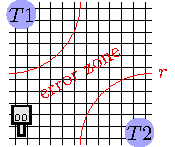
\includegraphics[width=.45\linewidth]{robotgrid.pdf} 
\visible<2->{
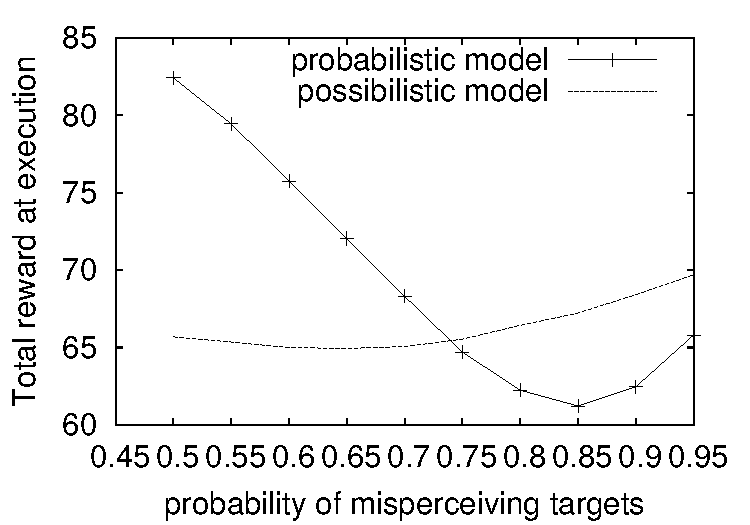
\includegraphics[width=.5\linewidth]{courbe1.pdf}\\
\vspace{0.2cm}
in reality, misperception probability in the error zone: $P_{bad} > \frac{1}{2}$
}
\end{exampleblock}
\visible<3->{
\grille
}
\end{frame}

\section[solver $\&$ factorization]{Symbolic solver and factorization}
\begin{frame}
\frametitle{Factored $\pi$-MOMDP and computations with ADDs}
\framesubtitle{\footnotesize qualitative possibilistic models to reduce complexity}
	\centering
	\begin{exampleblock}{}
	\textbf{contribution (AAAI-14):} factored $\pi$-MOMDP \\ 
$\Leftrightarrow$ state space $\mathcal{X} = \mathcal{S}_v \times \Pi_{\mathcal{L}}^{\mathcal{S}_h} =$ 
Boolean variables ($X_1,\ldots,X_n$) \\ 
	\hspace{1cm} $+$ independence assumptions $\Leftarrow$ graphical model
	\end{exampleblock}
	\vspace{0.2cm}
	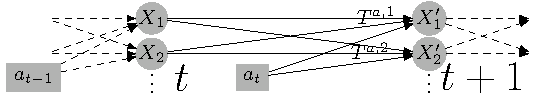
\includegraphics[scale=1]{factMDPdid.pdf} \\
	\visible<2->{
	%\vspace{0.5cm}
	\begin{alertblock}{}
	\centering
	\begin{minipage}{0.75\linewidth}
	\begin{itemize}
	\item \textbf{factorization:} transition functions $T_i^a = \pi \paren{X_i' \sachant parents(X_i'),a}$ stored as\\ 
	\textbf{Algebraic Decision Diagrams (ADD)} \\
	\vspace{0.3cm}
	probabilistic case:\\ 
	SPUDD { \footnotesize (\textit{Hoey et al., 1999})}
	\end{itemize}
	\end{minipage}
	\hspace{0.2cm}
	\begin{minipage}{0.2\linewidth}
	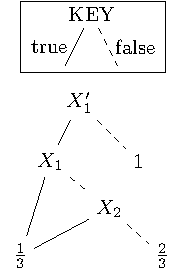
\includegraphics[scale=0.55]{tabADD} \\
	\scriptsize example of ADD
	\end{minipage} 
	\end{alertblock}
	}
\end{frame}




\begin{frame}
\frametitle{Simplify computations with $\pi$-MOMDPs}
\framesubtitle{\footnotesize Resulting $\pi$-MOMDP solver: PPUDD}
\centering
\begin{block}{}
\begin{itemize}
\item probabilistic model: $+$ and $\times$ $\Rightarrow$ new values created \\ 
$\Rightarrow$ number of ADDs leaves \textbf{potentially huge}
\item possibilistic model: $\min$ and $\max$ $\Rightarrow$ values $\in \mathcal{L}$ finite\\
$\Rightarrow$ number of leaves bounded, \textbf{ ADDs \textbf{smaller}}.
\end{itemize}
\end{block}
\visible<2->{
\begin{alertblock}{\textbf{PPUDD: Possibilistic Planning Using Decision Diagrams}}
\begin{itemize}
\item factorization $\Rightarrow$ each DP steps divided into $n$ stages\\ 
$\rightarrow$ smaller ADDs $\Rightarrow$ \textbf{faster computations}
}
\visible<3->{
\item computations on trees: \textit{CU Decision Diagram Package}.
}
\end{itemize}
\end{alertblock}
\end{frame}








 \newcommand{\grillesecond}{
 \begin{tikzpicture}[overlay,remember picture]
   \begin{scope}[shift={(current page.south west)}]
	\tikzstyle{vertexBIGRED}=[fill=red!30,draw=red, minimum width=320pt, minimum height=51pt,line width=1pt,inner sep=5pt,rounded corners]
	\node[vertexBIGRED] at (6.5,7) {};%};
	\node at (6,7.5) {$\perp\!\!\!\perp$ assumptions on state $\&$ observation variables};
	\node at (6.5,7) {$\rightarrow$ belief variable factorization};
	\node at (6.95,6.5) {$\rightarrow$ \textbf{additional} computation savings};
   \end{scope}
 \end{tikzpicture}
 }

\begin{frame}
\frametitle{Simplifying computations with $\pi$-MOMDPs}
\framesubtitle{\footnotesize Natural factorization: belief independence}
\vspace{0.02cm}
\textbf{contribution (AAAI-14):} 
\vspace{-0.2cm}
\begin{alertblock}{}
independent sensors, hidden states, $\ldots$ $\Rightarrow$ graphical model
\end{alertblock}
\vspace{-0.1cm}
\visible<2->{
d-Separation $\Rightarrow$ { \color{blue} $(s_v,\beta) = (s_{v,1}, \ldots, s_{v,m}, \beta_1, \ldots, \beta_{l})$} \\
\hspace{0.4cm} { \color{red} $\beta_i \in \Pi^{\mathcal{S}_{h,i}}_{\mathcal{L}}$, belief over $s_{h,i}$}
\vspace{-0.2cm}
}
\begin{tikzpicture}
\node at (-2.2cm,0cm) {};
\node at (0cm,9.9) {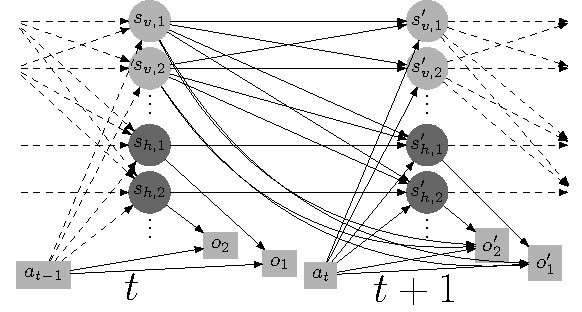
\includegraphics[scale=1]{factMOMDPdid.pdf}};
\visible<2->{
\tikzstyle{bvertex}=[circle,fill=red!60,minimum size=30pt,inner sep=0pt]

	\node[bvertex] (bel1) at (4.5,10.8) {\Large $\beta_1'$};
	\node[bvertex] (bel2) at (3.6,9.8) {\Large $\beta_2'$};
	\node (obs1) at (4.5,8.2) {};
	\node (obs2) at (3.6,8.5) {};
	\node (act) at (0.4,7.9) {};
	\draw[color=red!60,ultra thick,>=latex,->] (obs1) to (bel1); 
	\draw[color=red!60,ultra thick,>=latex,->] (obs2) to (bel2); 
	\draw[color=red!60,ultra thick,>=latex,->] (act) to [bend left] (bel1); 
	\draw[color=red!60,ultra thick,>=latex,->] (act) to [bend left] (bel2); 

	\node[bvertex] (bel11) at (-0.1,10.8) {\Large $\beta_1$};
	\node[bvertex] (bel21) at (-1,9.8) {\Large $\beta_2$};
	\node (obs11) at (-0.1,8.1) {};
	\node (obs21) at (-1,8.4) {};
	\node (act1) at (-4.1,7.9) {};
	\draw[color=red!60,ultra thick,>=latex,->] (obs11) to (bel11); 
	\draw[color=red!60,ultra thick,>=latex,->] (obs21) to (bel21); 
	\draw[color=red!60,ultra thick,>=latex,->] (act1) to [bend left] (bel11); 
	\draw[color=red!60,ultra thick,>=latex,->] (act1) to [bend left] (bel21); 

	\draw[color=red!60,ultra thick,>=latex,->] (bel11) to (bel1); 
	\draw[color=red!60,ultra thick,>=latex,->] (bel21) to (bel2); 


	\node (bel12) at (-5,10.8) {};
	\node (bel22) at (-5,9.8) {};
    	\draw[color=red!60,ultra thick,>=latex,->,dashed] (bel12) to (bel11); 
	\draw[color=red!60,ultra thick,>=latex,->,dashed] (bel22) to (bel21); 
}
\end{tikzpicture}
\visible<3->{
\grillesecond
}
\end{frame}

% observations


\begin{frame}
\frametitle{Simplify computations with $\pi$-MOMDPs}
\framesubtitle{\footnotesize Experiments -- perfect sensing: Navigation problem}
\vspace{-0.2cm}
\centering
\begin{exampleblock}{}
PPUDD vs SPUDD { \footnotesize (\textit{Hoey et al.}, 1999)} \\ 
{ \color{red!70} Navigation benchmark}: reach a goal -- spots with accident risk \\ 
M1 (resp. M2) optimistic (resp. pessimistic) criterion 	
\end{exampleblock}
\visible<2->{
\textbf{ Performances, function of the problem index }  \\
\vspace{0.2cm}
\begin{minipage}{0.45\linewidth}
\centering
{\color{orange} reached goal frequency} \\
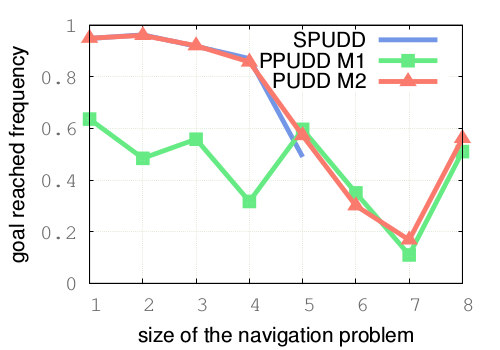
\includegraphics[scale=0.4]{courbePerfMDP.png} 
\end{minipage}
\begin{minipage}{0.45\linewidth}
\hspace{0.5cm}{\color{orange} $\#$ steps to reach the goal} \\
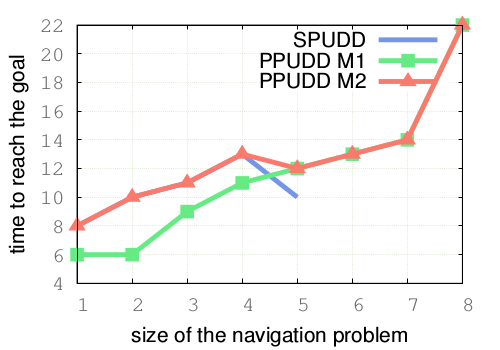
\includegraphics[scale=0.4]{courbePerfMDP2.png} 
\end{minipage}\\
\vspace{0.4cm} 
\definecolor{gggreen}{rgb}{0,0.7,0.7}
\hspace{1.2cm} {\color{gggreen} the higher the better} \hspace{1.4cm} {\color{gggreen} the lower the better}
}
\end{frame}


\begin{frame}
\frametitle{Simplify computations with $\pi$-MOMDPs}
\framesubtitle{\footnotesize Experiments -- perfect sensing: Navigation problem}
\begin{minipage}{0.45\linewidth}
\centering
{\color{orange} computation time} \\
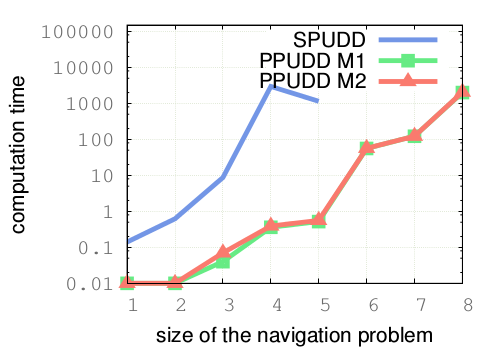
\includegraphics[scale=0.4]{courbeTime.png} 
\end{minipage}
\hspace{0.13cm}
\begin{minipage}{0.45\linewidth}
{\hspace{0.5cm} \color{orange} max size of ADDs} \\
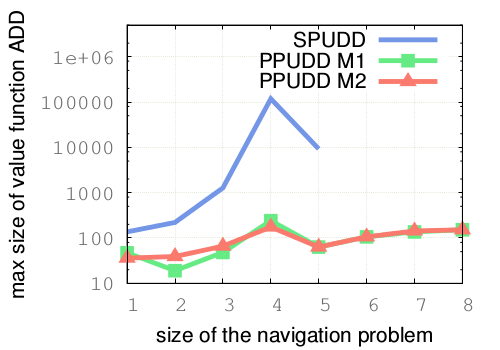
\includegraphics[scale=0.3]{courbeADD.png}  
\end{minipage}
\begin{alertblock}{}
\centering
\begin{itemize}
\item PPUDD + M2 (pessimistic criterion)\\ 
\textbf{faster with same performances} as SPUDD
\item SPUDD only solves the first $5$ instances
\item verified intuition: ADDs are smaller
\end{itemize}
\end{alertblock}
\end{frame}

\begin{frame}
\frametitle{Simplify computations with $\pi$-MOMDPs}
\framesubtitle{\footnotesize Experiments -- imperfect sensing: RockSample problem}
\vspace{-0.1cm}
	\begin{exampleblock}{}
	PPUDD vs APPL {\footnotesize (\textit{Kurniawati et al.}, 2008, solver MOMDP)} \\
 	\hspace{1cm} symbolic HSVI {\footnotesize ( \textit{Sim et al.}, 2008, solver POMDP)} \\
	{ \color{red!70} RockSample benchmark}: recognize and sample ``good'' rocks
	\end{exampleblock}
	\visible<2->{
\vspace{-0.05cm}
	\begin{minipage}{0.55\linewidth}
	\centering	
	{\color{orange} computation time:}\\ 
	\vspace{-0.05cm} {\footnotesize probabilistic solvers, prec. $1$} \\ 
	\vspace{-0.15cm} {\footnotesize PPUDD, exact resolution} \\
	\vspace{-0.05cm}
	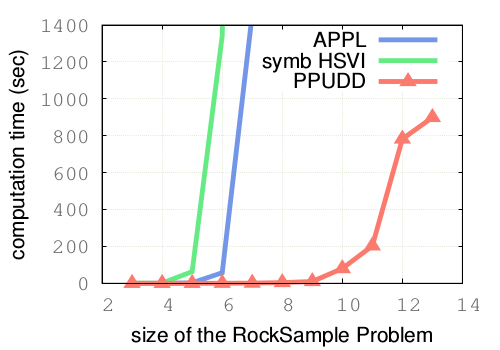
\includegraphics[scale=0.4]{RockSampleCompTime.png}
	\end{minipage}
	\hfill
	\begin{minipage}{0.43\linewidth}
	\centering
	{\color{orange} average of rewards} \\  
	{\footnotesize APPL stopped when \\ \vspace{-0.15cm} PPUDD end }\\
	\vspace{-0.03cm}
	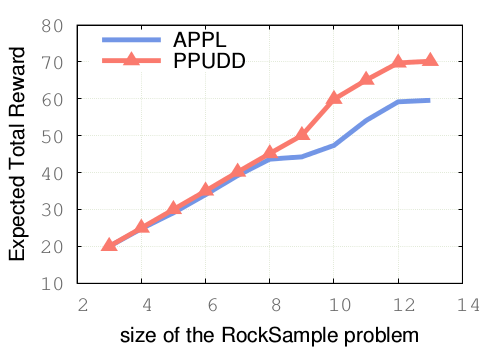
\includegraphics[scale=0.4]{courbePerfTime.png} 
	\end{minipage}

\vspace{-0.1cm}
\begin{alertblock}{}
\begin{itemize}
\item \textbf{approximate model} $+$ \textbf{exact resolution solver} \\
$\rightarrow$ improvement of computation time and performances
\end{itemize}
\end{alertblock}
}
\end{frame}




%%%%%%%%%%%%%%%%%%%%%%%%%%%%%%%%%%%%%%%%%%%%%%%%%%
%%%%%%%%%%%%%%%%%%%%%%%%%%%%%%%%%%%%%%%%%%%%%%%%%%
%%%%%%%%%%%%%%%%%%%%%%%%%%%%%%%%%%%%%%%%%%%%%%%%%%
%%%%%%%%%%%%%%%%%%%%%%%%%%%%%%%%%%%%%%%%%%%%%%%%%%
%%%%%%%%%%%%%%%%%%%%%%%%%%%%%%%%%%%%%%%%%%%%%%%%%%
%%%%%%%%%%%%%%%%%%%%%%%%%%%%%%%%%%%%%%%%%%%%%%%%%%
%%%%%%%%%%%%%%%%%%%%%%%%%%%%%%%%%%%%%%%%%%%%%%%%%%
%%%%%%%%%%%%%%%%%%%%%%%%%%%%%%%%%%%%%%%%%%%%%%%%%%
%%%%%%%%%%%%%%%%%%%%%%%%%%%%%%%%%%%%%%%%%%%%%%%%%%
%%%%%%%%%%%%%%%%%%%%%%%%%%%%%%%%%%%%%%%%%%%%%%%%%%
%%%%%%%%%%%%%%%%%%%%%%%%%%%%%%%%%%%%%%%%%%%%%%%%%%
%%%%%%%%%%%%%%%%%%%%%%%%%%%%%%%%%%%%%%%%%%%%%%%%%%
%%%%%%%%%%%%%%%%%%%%%%%%%%%%%%%%%%%%%%%%%%%%%%%%%%
%%%%%%%%%%%%%%%%%%%%%%%%%%%%%%%%%%%%%%%%%%%%%%%%%%
%%%%%%%%%%%%%%%%%%%%%%%%%%%%%%%%%%%%%%%%%%%%%%%%%%

%%%%%%%%%%%%%%%%%%%%%%%%%%%%%%%%%%%%%%%%%%%%%%%%%%
%%%%%%%%%%%%%%%%%%%%%%%%%%%%%%%%%%%%%%%%%%%%%%%%%%
%%%%%%%%%%%%%%%%%%%%%%%%%%%%%%%%%%%%%%%%%%%%%%%%%%
%%%%%%%%%%%%%%%%%%%%%%%%%%%%%%%%%%%%%%%%%%%%%%%%%%
%%%%%%%%%%%%%%%%%%%%%%%%%%%%%%%%%%%%%%%%%%%%%%%%%%
%%%%%%%%%%%%%%%%%%%%%%%%%%%%%%%%%%%%%%%%%%%%%%%%%%
%%%%%%%%%%%%%%%%%%%%%%%%%%%%%%%%%%%%%%%%%%%%%%%%%%
%%%%%%%%%%%%%%%%%%%%%%%%%%%%%%%%%%%%%%%%%%%%%%%%%%
%%%%%%%%%%%%%%%%%%%%%%%%%%%%%%%%%%%%%%%%%%%%%%%%%%
%%%%%%%%%%%%%%%%%%%%%%%%%%%%%%%%%%%%%%%%%%%%%%%%%%
%%%%%%%%%%%%%%%%%%%%%%%%%%%%%%%%%%%%%%%%%%%%%%%%%%
%%%%%%%%%%%%%%%%%%%%%%%%%%%%%%%%%%%%%%%%%%%%%%%%%%
%%%%%%%%%%%%%%%%%%%%%%%%%%%%%%%%%%%%%%%%%%%%%%%%%%
%%%%%%%%%%%%%%%%%%%%%%%%%%%%%%%%%%%%%%%%%%%%%%%%%%
%%%%%%%%%%%%%%%%%%%%%%%%%%%%%%%%%%%%%%%%%%%%%%%%%%
\nico{



\begin{frame}
\frametitle{IPPC 2014 -- ADD-based approaches:\\ 
PPUDD vs symbolic LRTDP}% (\textit{Bonet et al.})}
\vspace{-0.4cm}
PPUDD $+$ BDD mask over reachable states. \\
\vspace{-0.6cm}
\begin{figure}
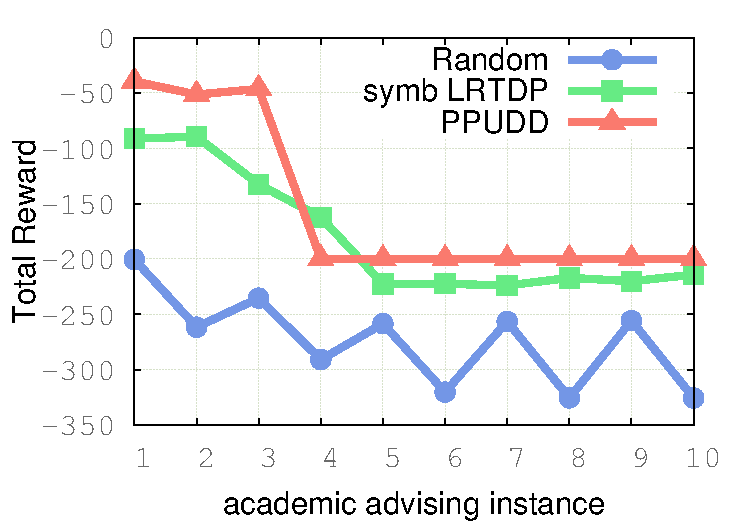
\includegraphics[scale=0.3]{IPPC2014_results/academic_advising.pdf}
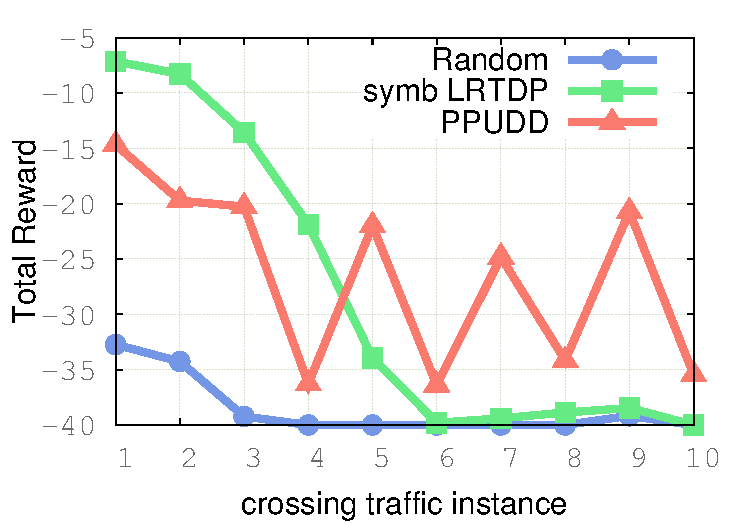
\includegraphics[scale=0.3]{IPPC2014_results/crossing_traffic.pdf} 
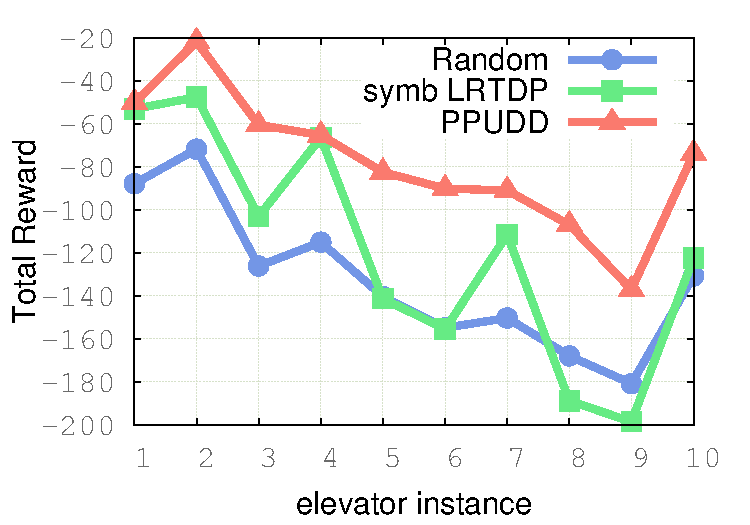
\includegraphics[scale=0.3]{IPPC2014_results/elevator.pdf} \\
\vspace{0.5cm}
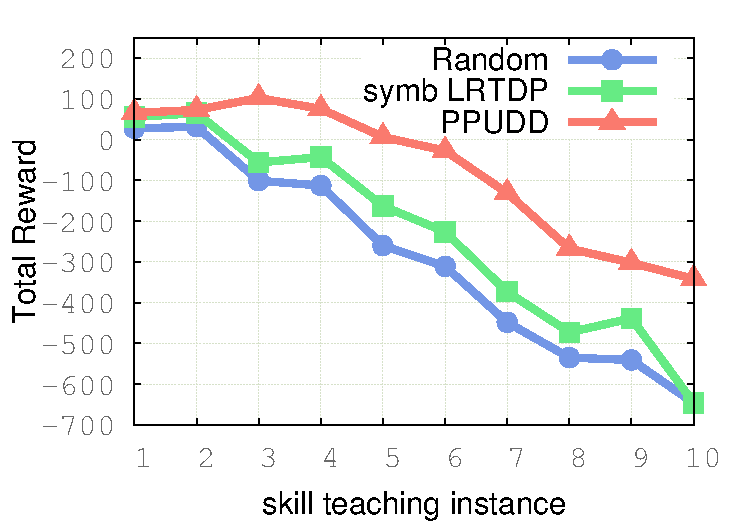
\includegraphics[scale=0.3]{IPPC2014_results/skill_teaching.pdf} 
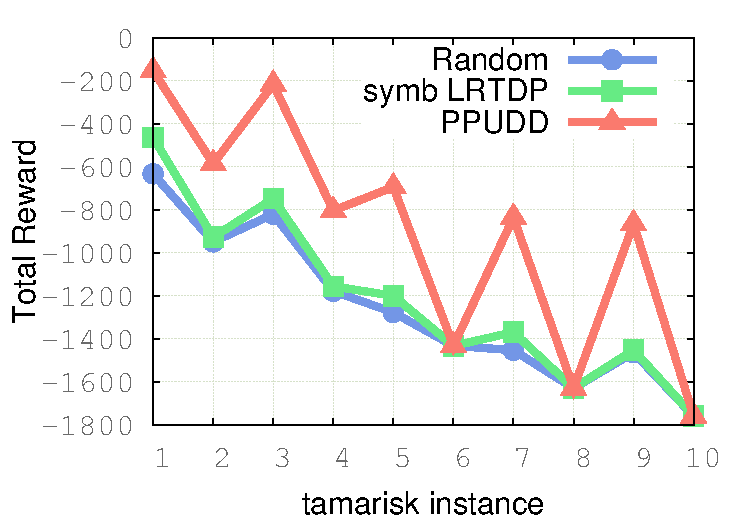
\includegraphics[scale=0.3]{IPPC2014_results/tamarisk.pdf}
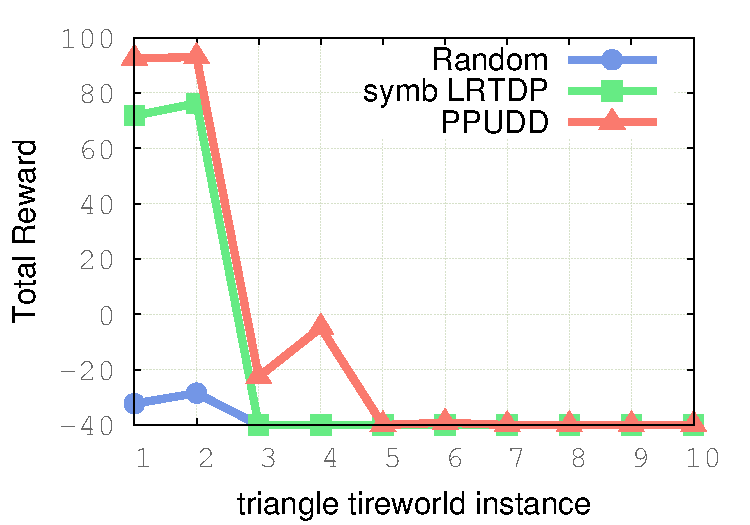
\includegraphics[scale=0.3]{IPPC2014_results/triangle_tireworld.pdf} 
\caption{{\color{orange} average of rewards over simulations}}
\end{figure}
\end{frame}

\nico{ %% INTERACTIVE PROOF
%\section{Belief factorization}
\begin{frame}

\frametitle{Independent beliefs}
\vspace{-0.85cm}
\hspace{5cm} \textit{A $\pi$-MOMDP fulfilling assumptions of the Dynamic Bayesian Network below has a} \textbf{natural factorization}: \\ { \color{blue} $(s_v,\beta) = (s_{v,1}, \ldots, s_{v,m}, \beta_1, \ldots, \beta_{l})$}, with $\beta_i$ belief about $s_{h,i}$. \\
\visible<2->{
\vspace{-0.2cm}
\begin{alertblock}{}
{ \color{red} some assumptions:} one observation variable for each hidden state variable, hidden state variables independent on other hidden state variables ...
\end{alertblock}
\vspace{-0.2cm}
}
\begin{center}
\hspace{1.35cm}
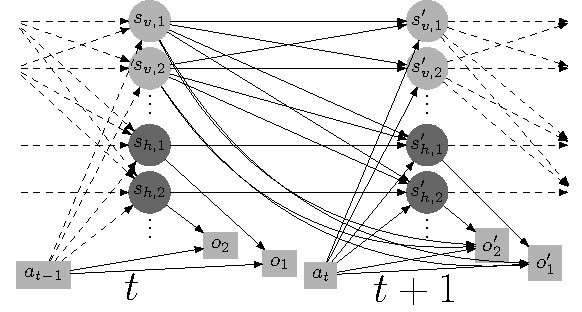
\includegraphics[scale=1]{factMOMDPdid.pdf}
\end{center}
\end{frame}

\begin{frame}
	\textit{beginning of the proof}:
\begin{itemize} 
		\item $\forall 1 \leqslant i < j \leqslant l$, $s_{h,i}$ and $s_{h,j}$ are \textbf{$d$-separated} by evidence $h_t$ (history) 
	\end{itemize}
	\visible<13->
	{
		 $\rightarrow$ for each time $t$,  hidden state variables $s_{h,i}$ are independent given $h_t$
		\[ \mbox{ i.e. } { \color{blue} \beta_t(s_h) } = \pi \paren{ s_h \sachant h_t} = \displaystyle \min_i \pi \paren{s_{h,i} \sachant h_t} = { \color{blue} \displaystyle \min_i \beta_{t,i}(s_{h,i}) } \]
		\vspace{-0.3cm}
	}
\begin{figure}[b]\centering
\begin{tikzpicture}
	\visible<2->
	{
	\draw[ultra thick,green!50] (-5,12.7) -- (3,12.7) -- (3,10.7) -- (-3.2,10.7) ;
	\draw[ultra thick,green!50] (-3.2,8.8) -- (4.8,8.8) -- (4.8,7.4) -- (-5, 7.4) ;
	\draw[ultra thick,green!50,dashed] (-3.2,8.8) -- (-5,8.8);
	\draw[ultra thick,green!50,dashed] (-3.2,10.7) -- (-5, 10.7);
	\draw[ultra thick,green!50,dashed] (-6.5,12.7) -- (-5,12.7);
	\draw[ultra thick,green!50,dashed] (-6.5,7.4) -- (-5,7.4);
	\node[green!60] (ev) at (-5.5,12.4) {evidence:};
	\node[green!60] (ev2) at (-5.5,11.9) {\textbf{history} $h_t$};
		
	\draw[ultra thick,red!60] (2.305,10.06) circle (0.375cm);
	\draw[ultra thick,red!60] (2.305,9.26) circle (0.375cm);
	
	}
	\visible<3-4>
	{
		\draw[ultra thick,>=latex,->,red!60] (2,10.2) -- (-2,12);
		\draw[ultra thick,>=latex,->,red!60] (2,10.15) -- (-2,11.25);	
		\node[red!70] at (-1.45,12.4) { \scriptsize blocked};
		\draw[very thick,red!60] (-2.8,12.6) -- (-2,12.6) -- (-2,10.9) -- (-2.8,10.9) -- (-2.8,12.6) ;
	}
	\visible<4->
	{
		\node (check) at (1.4,10.5) {
\includegraphics[scale=0.022]{crossCheck.png}};	
		\node (check) at (1,10.45) {
\includegraphics[scale=0.022]{crossCheck.png}};	
	}
	
	\visible<5-7>
	{
		\draw[ultra thick,>=latex,->,red!60] (2,10.07) -- (-2,10.07);
	}

	\visible<6-7>
	{
			\draw[ultra thick,>=latex,->,red!60] (-2.5,10.07) -- (-5,10.07);
			\draw[ultra thick,>=latex,->,red!60] (-2.45,10.1) -- (-4.85,11.45);
			\draw[ultra thick,>=latex,->,red!60] (-2.42,10.1) -- (-4.32,11.85);
			\node[red!70] at (-5,11) { \scriptsize blocked};	
	}
	
	\visible<7->
	{
		%\draw[ultra thick,>=latex,->,red!60] (2,11.97) -- (-2,9.5);
		%\draw[ultra thick,>=latex,->,red!60] (2,11.22) -- (-2,9.43);
		\node (check) at (1.25,10.08) {
\includegraphics[scale=0.022]{crossCheck.png}};	
	}
	\visible<8-9>
	{
		\draw[ultra thick,>=latex,->,red!60] (2.2,9.95) -- (0.7,8.1);
		\node[red!70] at (0.1,8.5) { \scriptsize blocked};
		\draw[very thick,red!60] (0.17,7.6) -- (0.83,7.6) -- (0.83,8.15) -- (0.19,8.15) -- (0.19,7.6) ;
	}
	\visible<9->
	{
		\node (check) at (1.4,9) {
\includegraphics[scale=0.022]{crossCheck.png}};	
	}
	\visible<10-12>
	{
		\draw[ultra thick,>=latex,->,red!60] (2.4,9.98) -- (4,8.38);
		%\draw[ultra thick,>=latex,->,red!60] (2,11.35) -- (-2,11.35);	
		%\draw[ultra thick,>=latex,->,red!60] (2,12.1) -- (-2,11.45);
	}
	\visible<11-12>
	{
		\draw[ultra thick,>=latex,->,red!60] (4,8.05) -- (0.7,7.88);
		\node[red!70] at (0.1,8.5) { \scriptsize blocked};
		\draw[very thick,red!60] (0.17,7.6) -- (0.83,7.6) -- (0.83,8.15) -- (0.19,8.15) -- (0.19,7.6) ;
	}
	\visible<12->
	{
		\node (check) at (2.9,9.5) {
\includegraphics[scale=0.022]{crossCheck.png}};	
	}
	\node (factMOMDP) at (0,9.88) {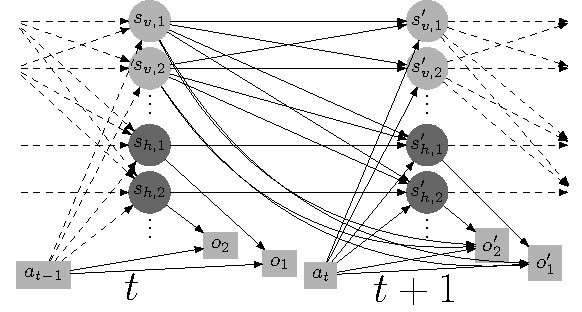
\includegraphics[scale=1]{factMOMDPdid.pdf}};
\end{tikzpicture}
\end{figure}
\end{frame}
} %%%% FIN INTERACTIVE PROOF


\section[hybrid model]{A hybrid model} 
\begin{frame}
\frametitle{Qualitative possibilistic approach: benefits/drawbacks} 
\framesubtitle{\footnotesize towards a hybrid POMDP}
\begin{block}{}
\begin{itemize}
\item \textbf{granulated} belief space (discrete)% representation\\% (discretization)\\ 
%\hspace{2.03cm} 
\item efficient problem \textbf{simplification} (PPUDD $2 \times$ better \\
\hspace{5cm} than LRTDP with ADDs)
\item \textbf{ignorance and imprecision} modeling
\end{itemize}
\end{block}
\visible<2->{
\begin{alertblock}{}
\begin{itemize} 
\item ADD methods $\prec$ state space search methods \\
$\rightarrow$ winners of IPPC 2014: $2 \times$ better than PPUDD \\
\item choice of the qualitative criterion (optimistic/pessimistic)
\item preference $\rightarrow$ non additive degrees\\ 
$\rightarrow$ same scale as possibility degrees (commensurability)
\item coarse approximation of probabilistic model\\ 
$\rightarrow$ no frequentist information
\end{itemize}
\end{alertblock}
}
\end{frame}


\begin{frame}
\frametitle{A hybrid model}
\framesubtitle{\footnotesize a probabilistic POMDP with possibilistic belief states}
\begin{block}{hybrid approach}
\begin{itemize}
\item agent knowledge = possibilistic belief states 
\item probabilistic dynamics $\&$ quantitative rewards
%\item traduction PSCACE $\rightarrow$ EXPTIME car $\# \Pi_S \sim \# \mathcal{L}^{\# \mathcal{S}}$.
\end{itemize}
\end{block}

\visible<2->{
\begin{alertblock}{Usefullness}
$\rightarrow$ \textbf{heuristic} for solving POMDPs:\\ 
\hspace{1cm} results in a standard (finite state space) MDP \\
$\rightarrow$ problem with \textbf{qualitative $\&$ quantitative} uncertainty\\
\end{alertblock}

}

\end{frame}





\begin{frame}
\frametitle{Transitions and rewards}
\framesubtitle{\footnotesize belief-based transition and reward functions}
%\begin{alertblock}{}
%\begin{itemize}
%\item {\color{red} problem of defining possibilistic distributions and $\mathcal{L}$}:\\
%\begin{enumerate}
%\item 
%$\mathbb{P} \rightarrow \pi$ transformations: 
%pignistic, specific, $\ldots$
%\item %probabilités estimées avec garantie faible\\ 
%POMDP décrit plus fidèlement par $\pi$.
%\end{enumerate} 
%\end{itemize}
%\end{alertblock}

\begin{itemize}
\item possibility distribution $\beta \rightarrow$ probability distribution $\overline{\beta}$\\ 
using poss-prob tranformations {\footnotesize \textit{(Dubois et al., FSS-92)}}% $\textbf{p} \paren{ o' \sachant s,a } = \sum_{s' \in \mathcal{S}} O(s',a,o') \cdot T(s,a,s');$
%\item observation probability $\textbf{p}\paren{o'\sachant \beta,a}$ computed from $\overline{b^{\pi}}$\\
%as usual since $\overline{b^{\pi}} =$ probabilistic belief 
%\item { \color{red} $ \displaystyle \textbf{p}\paren{o'\sachant b^{\pi},a} := \sum_{s\in\mathcal{S}}\textbf{p}\paren{o' \sachant s,a}\cdot\overline{b^{\pi}}(s)$.}
\end{itemize}
\begin{block}{Transition function on belief states}
\[ \Rightarrow \textbf{p} \Big( \beta' \Big\vert \overline{\beta},a \Big) = \sum_{ \substack{ o' \mbox{ \footnotesize t.q. } \\ update(\beta,a,o')=\beta'} }\textbf{p}\paren{o'\sachant \overline{\beta},a}\]
\end{block}
%\vspace{0.5cm}
%notation: if $a \in \mathcal{A}$ selected, $o' \in \mathcal{O}$ received,\\ 
%\[ b^{\pi}_{t+1} = u \paren{o',a,b^{\pi}_t} = \mbox{ update of } b^{\pi}_t. \]
\visible<2->{
\begin{itemize}
\item reward cautious according to $\beta$
\end{itemize}
\begin{block}{Pessimistic Choquet Integral}
\[ r(\beta,a) = \sum_{i=1}^{\# \mathcal{L}-1} (l_i - l_{i+1}) \cdot \hspace{-0.1cm} \min_{ \substack{ s \in \mathcal{S} \mbox{ \scriptsize  s.t. } \\ \beta(s) \geqslant l_i } }  r(s,a) \]
\end{block}
}

\end{frame}


\begin{frame}
\frametitle{Resulting MDP}
\framesubtitle{\footnotesize translation from hybrid POMDP to MDP -- \textbf{contribution (SUM-15):}}
\vspace{0.3cm}
input: a POMDP $\langle \mathcal{S},\mathcal{A},\mathcal{O},T,O,r, \gamma \rangle$ \\
output: the MDP $\langle \tilde{\mathcal{S}},\mathcal{A},\tilde{T},\tilde{r}, \gamma \rangle$:
\vspace{0.3cm}
\visible<2->{
\begin{itemize}
\item \textbf{state space} ${ \color{red} \tilde{\mathcal{S}} = \Pi_{\mathcal{L}}^{\mathcal{S}} }$,\\ 
the set of the possibility distributions over $\mathcal{S}$
\end{itemize}
}
\vspace{0.3cm}
\visible<3->{
\begin{itemize}
\item $\forall \beta, \beta'$ possibilistic belief states $\in \Pi^{\mathcal{S}}_{\mathcal{L}}$, $\forall a \in \mathcal{A}$,\\
\textbf{transitions} ${ \color{red} \tilde{T} \Big( \beta, a, \beta' \Big) = \textbf{p} \Big( \beta' \Big\vert \beta,a \Big) }$
\end{itemize}
}
\vspace{0.3cm}
\visible<4->{
\begin{itemize}
\item \textbf{reward} ${ \color{red}  \tilde{r}(a,\beta) = \underline{Ch} \Big( r(a,.) \Big) }$,\\ 
%$\mathcal{N}_{\beta}$ necessity measure computed from $\beta$.
\end{itemize}
}
\vspace{0.2cm}
\visible<5->{
\[ \mbox{ \textbf{criterion:} } \mathbb{E}_{ \beta_t \sim \tilde{T}} \croch{ \sum_{t=0}^{+ \infty} \gamma^t \cdot \tilde{r} \paren{ \beta_t,d_t } }.\]
}
\end{frame}

\begin{frame}
\frametitle{General variable classification {\footnotesize \textbf{contribution (SUM-15):}}}
\framesubtitle{\footnotesize $3$ classes of state variables -- state space factorization}%: extension des MOMDPs (Araya-L\'opez, Ong)}
\vspace{0.1cm}
\begin{tikzpicture}
\definecolor{violet}{rgb}{0.7,0.1,0.5};
\definecolor{orangee}{rgb}{1,0.7,0.1};
\definecolor{gggreen}{rgb}{0,0.7,0.7};
% separations
\node (T1) at (-1.5,8.4) {};
\node (B1) at (9,8.4) {};
\draw[thick,dashed,color=black!30] (B1) to (T1);
\node (T2) at (-1.5,5.1) {};
\node (B2) at (9,5.1) {};
\draw[thick,color=black!30] (B2) to (T2);

% variables
\tikzstyle{vertex}=[circle,fill=black!30,minimum size=20pt,inner sep=0pt]
\node (V) at (1,10) { \underline{variable:} \color{violet} \textbf{visible} $s_v' \in \mathbb{S}_v$ };
\node[vertex] (vv) at (6.5,9.7) {$s_v'$};
\node (IHV) at (1.2,8) { {\color{gggreen} \textbf{inferred hidden} $ s_h' \in \mathbb{S}_h$} };
\node[vertex] (ihv) at (6.5, 7.15) {$s_h'$};
\node (FHV) at (1.5,4.75) { {\color{orangee} \textbf{fully hidden} $s_f' \in \mathbb{S}_f$}};
\node[vertex] (fhv) at (6.5,4) {$s_f'$};

\visible<2->{
% visible
\node[vertex] (ov) at (8.5,9.7) {$o_v'$};
\draw[->,>=latex,thick] (vv) to (ov);
\node at (7.5,10) {$s_v'= o_v'$};
}
\visible<3->{
\node (leg1) at (3.5,8.9) { \color{violet} $\beta_{t+1}(s_v') = \mathds{1}_{ \set{s_v'=o_v'} }(s_v')$ };
}
\visible<4->{
\node (leg1) at (2,9.5) { $\Leftrightarrow$ deterministic belief variable };
}

\visible<5->{
% inférée
\tikzstyle{hvertex}=[circle,fill=black!10,minimum size=20pt,inner sep=0pt]
\node[vertex] (oh) at (8.5,7.15) {$o_i'$};
\draw[->,>=latex,thick] (ihv) to (oh);
\node[hvertex] (sh1) at (6.5,8) {$s_h^{a}$};
\node[hvertex] (sh2) at (6.8,6.2) {$s_h^{b}$};
\node[hvertex] (sh3) at (7.5,5.5) {$s_h^{c}$};
\draw[->,>=latex,thick,dashed] (sh1) to (oh);
\draw[->,>=latex,thick,dashed] (sh2) to (oh);
\draw[->,>=latex,thick,dashed] (sh3) to (oh);
}

\visible<6->{
\node (leg2) at (2,7.3) {$ {\color{gggreen} \beta_{t+1}\Big(parents(o_i')\Big) }= \beta_{t+1}(s_h,s_h^a,s_h^b,s_h^c)$};
}
\visible<7->{

\node (leg2) at (3.2,6.4) {$  {\color{gggreen} \propto^{\pi} \pi \Big( o_i', parents(o_i') \Big\vert \beta_t, a \Big)}$}; 
%\node (leg2) at (2.5,6.3) { $ \displaystyle \propto^{\pi} \hspace{-0.1cm} \max_{2^{\mathcal{Q}(o_i')}} \hspace{-0.1cm} \Bigg\{ \hspace{-0.1cm} \pi \hspace{-0.05cm} \Big( \hspace{-0.05cm}  o_i', \hspace{-0.05cm}  \mathcal{P}(o_i') \hspace{-0.02cm}  \Big\vert \hspace{-0.02cm}  \mathcal{Q}(o_i'), \hspace{-0.05cm}  a \hspace{-0.05cm}  \Big), \hspace{-0.1cm}  b^{\pi}_t \hspace{-0.1cm}  \Big( \hspace{-0.1cm}  \mathcal{Q}(o_i') \hspace{-0.1cm} \Big) \hspace{-0.1cm}  \Bigg\}$.}; 
}
\visible<8->{
\node (leg2) at (2.5,5.5) { { \color{red} {\fontencoding{U}\fontfamily{futs}\selectfont\char 66\relax}} $\mathcal{P}(o_i')$ may contain visible variables.};
}

\visible<9->{
% inférée
\tikzstyle{hvertex}=[circle,fill=black!10,minimum size=20pt,inner sep=0pt]
\node[vertex] (oh) at (8.5,4) {$o_i'$};
\draw[->,>=latex,thick] (fhv) to (oh);
\node (cross) at (7.5,4) {
\includegraphics[scale=0.033]{crossCheck}};
}
\visible<10->{
% inférée
\node (leg3) at (3.3,3.05) { { \color{orangee} $\beta_{t+1}(s_f') = \pi \paren{ s_f' \sachant \beta_t, a }$ } };
% \displaystyle \max_{2^{\mathcal{P}(s_f')}} \min \bigg\{ \pi \big( s_f'  \big\vert  \mathcal{P}(s_f'), \hspace{-0.1cm} a \big) , b^{\pi}_{t} \big(\mathcal{P}(s_f') \big) \bigg\} $}.};
}
\visible<11->{
\node (leg3) at (2,4.25) {$\rightarrow$ observations don't };
\node (leg3) at (2,3.75) { inform belief state on $s_f'$.};
}
\end{tikzpicture}
\end{frame}


\begin{frame}
\frametitle{Possibilistic belief variables}
\framesubtitle{\footnotesize global belief state}
\definecolor{violet}{rgb}{0.7,0.1,0.5}
\definecolor{orangee}{rgb}{1,0.7,0.1}
\definecolor{gggreen}{rgb}{0,0.7,0.7}
\definecolor{bblue}{rgb}{0,0.4,0.75}
%$\mathbb{O}_h = \mathbb{O} \setminus \mathbb{S}_v$.
\begin{block}{bound over the global belief state}
$\beta_{t+1}(s_1',\ldots,s_n') = \pi \paren{ s_1',\ldots,s_n' \sachant a_0,o_1, \ldots, a_{t},o_{t+1} } $
\end{block}
\hspace{0.5cm} $ \leqslant \displaystyle \min \hspace{-0.1cm} \Bigg\{ \hspace{-0.1cm} 
{\color{violet} \min_{s_j' \in \mathbb{S}_v} \hspace{-0.1cm} \bigg[ \mathds{1}_{ \set{s_j'=o_j'}} \bigg]} \hspace{-0.1cm}, 
{\color{orangee} \min_{s_j' \in \mathbb{S}_f} \hspace{-0.1cm} \bigg[ \beta_{t+1}(s_j') \bigg]} \hspace{-0.1cm} , \hspace{-0.1cm} 
{\color{gggreen} \min_{o_i' \in \mathbb{O}_h} \hspace{-0.1cm} \bigg[ \beta_{t+1} \Big( \hspace{-0.1cm} parents(o_i') 
\hspace{-0.1cm} \Big) \bigg]} \hspace{-0.1cm}  \Bigg\} \hspace{-0.3cm}$\\
\visible<2->{
\vspace{1cm}
\begin{itemize}
\item $\min$ of marginals $=$ a \textbf{less informative} belief state
\item computed using \textbf{marginal belief states}\\ 
$\rightarrow$ { \color{red} factorization \& smaller state space}
\end{itemize}
}
%en possibiliste, pas besoin d'enlever les $\mathcal{P}(o_i')$ grâce au min!\\
%The possibilistic normalization, $\forall w \in 2^{\mathcal{P}(o_i')}$,
%$b'(w) = \left \{ \begin{array}{ccc} 1 \mbox{ if } w \in \operatorname*{argmax}_{v \in 2^{\mathcal{P}(o_i')}} \tilde{b}'(v); \\
% \tilde{b}'(w) \mbox{ otherwise} . \end{array} \right.$ 
\end{frame}



\section[conclusion]{Conclusion/Perspectives}

\begin{frame}
\frametitle{Conclusion}
\framesubtitle{\footnotesize contributions}
\vspace{0.1cm}
\begin{block}{}
\begin{itemize}
\item \textbf{modeling efforts}: $\rightarrow$ human-machine interaction
\visible<2->{
\item \textbf{advancements}: $\rightarrow$ mixed-observability modeling\\
\hspace{1.3cm} $\rightarrow$ indefinite horizon + optimality proof
}
\visible<3->{
\item \textbf{simplifying computations}: factorization work\\ 
\hspace{5cm} $\&$ PPUDD algorithm 
}
\visible<4->{
\item \textbf{experimentations}: real problems \\
$\rightarrow$ robust recognition mission with possibilistic beliefs\\
$\rightarrow$ validation of the computation time reduction\\
$\rightarrow$ IPPC 2014 
}
\visible<5->{
\item \textbf{hybrid POMDP} $\xrightarrow{ \mbox{\footnotesize translation} }$ MDP\\
$\rightarrow$ probabilities on possibilistic belief states\\ 
\hspace{0.4cm} pessimistic rewards (Choquet integral)\\
$\rightarrow$ factored POMDP $\xrightarrow{ \mbox{\footnotesize translation} }$ factored MPD
}
\end{itemize}
\end{block}


\end{frame}


\begin{frame}
\frametitle{Conclusion}
\framesubtitle{\footnotesize perspectives}

\begin{exampleblock}{}
\begin{itemize}
\item refined criteria {\footnotesize \textit{(Weng 2005, Dubois et al. 2005)}}\\ 
\hspace{2cm} $\Rightarrow$ finer $\pi$-POMDP \\
\item link with statistical learning in practice
\end{itemize}
\end{exampleblock}

\visible<2->{
\begin{alertblock}{}
quantitative information may be available: hybrid work
\end{alertblock}
\begin{itemize}
\item IPPC problems (factored POMDPs);
\item tests of this approach: 
\begin{enumerate}
\item \textbf{simplification:} $\pi$ distributions definition?%\\
%%($\pi$-normalization, pignistic transformation,\\ 
%most specific, \ldots);
\item \textbf{imprecision:} robust in practice?
\end{enumerate}
\end{itemize}
}
\end{frame}



}
%%%%%%%%%%%%%%%%%%%%%%%%%%%%%%%%%%%%%%%%%%%%%%%%%%
%%%%%%%%%%%%%%%%%%%%%%%%%%%%%%%%%%%%%%%%%%%%%%%%%%
%%%%%%%%%%%%%%%%%%%%%%%%%%%%%%%%%%%%%%%%%%%%%%%%%%
%%%%%%%%%%%%%%%%%%%%%%%%%%%%%%%%%%%%%%%%%%%%%%%%%%
%%%%%%%%%%%%%%%%%%%%%%%%%%%%%%%%%%%%%%%%%%%%%%%%%%
%%%%%%%%%%%%%%%%%%%%%%%%%%%%%%%%%%%%%%%%%%%%%%%%%%
%%%%%%%%%%%%%%%%%%%%%%%%%%%%%%%%%%%%%%%%%%%%%%%%%%
%%%%%%%%%%%%%%%%%%%%%%%%%%%%%%%%%%%%%%%%%%%%%%%%%%
%%%%%%%%%%%%%%%%%%%%%%%%%%%%%%%%%%%%%%%%%%%%%%%%%%
%%%%%%%%%%%%%%%%%%%%%%%%%%%%%%%%%%%%%%%%%%%%%%%%%%
%%%%%%%%%%%%%%%%%%%%%%%%%%%%%%%%%%%%%%%%%%%%%%%%%%
%%%%%%%%%%%%%%%%%%%%%%%%%%%%%%%%%%%%%%%%%%%%%%%%%%
%%%%%%%%%%%%%%%%%%%%%%%%%%%%%%%%%%%%%%%%%%%%%%%%%%
%%%%%%%%%%%%%%%%%%%%%%%%%%%%%%%%%%%%%%%%%%%%%%%%%%
%%%%%%%%%%%%%%%%%%%%%%%%%%%%%%%%%%%%%%%%%%%%%%%%%%

% questions
\frame{
\frametitle{\hspace{0.5cm}  
\includegraphics[scale=0.35]{logo2015} \hspace{0.7cm}  
\begin{tikzpicture}
\node[opacity=0.2] at (0,0) { 
\includegraphics[scale=0.32]{Logo_EDSYS2}};
\end{tikzpicture}
\hspace{0.6cm} 
\includegraphics[scale=0.5]{onera}  }
\vspace{-0.1cm}
{\Huge \textbf{Thank you!} }\\
\vspace{0.3cm}
produced work:
\begin{itemize}
\item \textit{Qualitative {P}ossibilistic {M}ixed-{O}bservable {MDP}s}, \textbf{UAI-2013}
\item \textit{Structured Possibilistic Planning Using Decision Diagrams}, \textbf{AAAI-2014}
\item \textit{Planning in Partially Observable Domains with Fuzzy Epistemic States and Probabilistic Dynamics}, \textbf{SUM-2015}
\item \textit{Processus D\'ecisionnels de Markov Possibilistes \`a Observabilit\'e Mixte}, Revue d'Intelligence Artificielle\\ (\textbf{RIA journal})
\item \textit{A Possibilistic Estimation of Human Attentional Errors}, submitted to \textbf{IEEE-TFS journal}
\end{itemize}

}
































































\nico{
\begin{frame}
\frametitle{Uncertainty theories}
\framesubtitle{\footnotesize Most known uncertainty theories and their relations}
\begin{figure} \centering
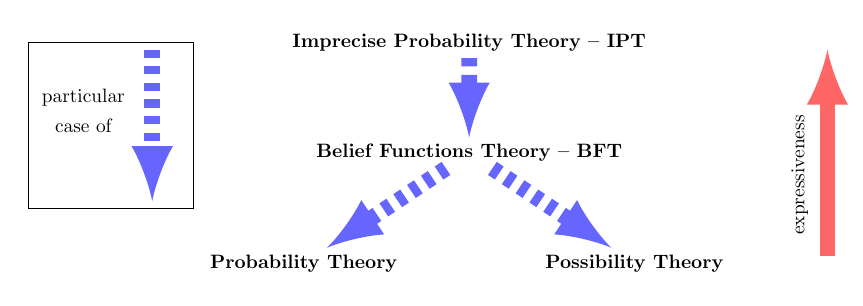
\begin{tikzpicture}[scale=0.7,transform shape]
\node (IP) at (2,10) {\textbf{Imprecise Probability Theory -- IPT}};
\node (BF) at (2,8) {\textbf{Belief Functions Theory -- BFT}};
\node (PROB) at (-1,6) {\textbf{Probability Theory}};
\node (POSS) at (5,6) {\textbf{Possibility Theory} };
\draw[->,>=latex,thick, color=blue!60, line width=2mm, dashed] (IP) to (BF);
\draw[->,>=latex,thick, color=blue!60, line width=2mm, dashed] (BF) to (PROB);
\draw[->,>=latex,thick, color=blue!60, line width=2mm, dashed] (BF) to (POSS);

\node (topr) at (8.5,10) {};
\node (botr) at (8.5,6) {};
\node (middr) at (8,7.6) [rotate=90] {expressiveness};
\draw[->,>=latex,thick, color=red!60, line width=2mm] (botr) to (topr);
\draw (-6,7) rectangle (-3,10);
\node (toplegend) at (-3.75,10) {};
\node (botlegend) at (-3.75,7) {};
\draw[->,>=latex,thick, color=blue!60, line width=2mm, dashed] (toplegend) to (botlegend);
\node (bluelegend) at (-5,9) {particular};
\node (bluelegend) at (-5,8.5) {case of};
\end{tikzpicture}
\end{figure}
\begin{itemize}
\item IPT: most general uncertainty theory.\\
Use of sets of probability measures over $\Omega$.
%defined on the universe $\Omega$ 
%in order to represent uncertainty of events 
%and knowledge about it: 
%this theory is 
\item BFT:
%which is a particular case of IPT, 
use of a mass function $m: 2^{\Omega} \rightarrow [0,1]$, \\
with $\sum_{A \subset \Omega} m(A)=1$. \\
%From this mass function,
%upper and lower bounds
%on possible probability measures
%can be defined. 
%The upper bound is called
\begin{enumerate}
\item plausibility measure: $\forall A \subset \Omega$, 
$Pl(A) = \sum_{B \cap A \neq \emptyset} m(B)$.
\item  belief function:
$\forall A \subset \Omega$, 
$bel(A) = \sum_{B \subseteq A} m(B)$.
\end{enumerate}
%The set of probability distributions
%represented by $m$ 
%are all probability measures $\mathbb{P}$
%such that $\forall A \subset \Omega$,
%$bel(A) \leqslant \mathbb{P}(A) \leqslant Pl(A)$.
%For instance, 
%if the function $m$ returns $1$ for the universe,
%and $0$ for all other subsets, 
%it expresses the total ignorance 
%about the actual probability distribution:
%it corresponds to the set of all the possible 
%probability distributions in IPT.
\end{itemize}
\end{frame}

\begin{frame}
\frametitle{Focal sets of a mass function $m:2^{\Omega} \rightarrow [0,1]$:\\
subsets $A$ of $\Omega = \set{ \omega_1,\ldots,\omega_7}$ such that $m(A)>0$.}
\begin{itemize}
\item if focal sets are all singletons\\ 
$\rightarrow$ probability distribution ($bel=Pl=\mathbb{P}$)
\item if focal sets are nested, e.g. $F_3 \subset F_2 \subset F_1 = \Omega$,\\ 
$\rightarrow$ 
%it corresponds to a 
possibility distribution:\\
$bel$=%is then called the 
\textbf{necessity measure},
%and 
$Pl$=%the 
\textbf{possibility measure}.% (see Section \ref{posspres} of Chapter \ref{chap_SOTA})
%Probability and Possibility Theories are thus
%particular cases of BFT and a fortiori of IPT.
\end{itemize}

\begin{figure}

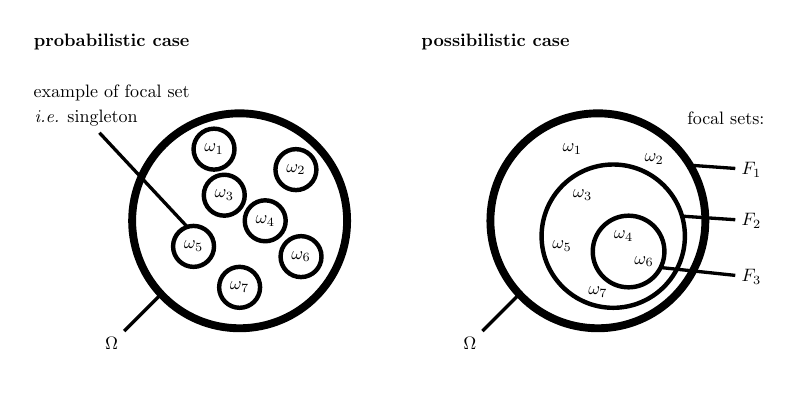
\begin{tikzpicture}[scale=0.65, transform shape]
\draw[line width=1mm] (0,2) circle (2.1cm);
\node at (-0.5  , 3.4) {$\omega_1$};
\node at (1.2, 1.3) {$\omega_6$};
\node at (1.1, 3) {$\omega_2$};
\node at (0  , 0.7) {$\omega_7$};
\node at (0.5  , 2) {$\omega_4$};
\node at (-0.9  , 1.5) {$\omega_5$};
\node at (-0.3  , 2.5) {$\omega_3$};
\draw[ultra thick] (-0.5  , 3.4) circle (0.4cm);
\draw[ultra thick] (1.2, 1.3) circle (0.4cm);
\draw[ultra thick] (1.1, 3) circle (0.4cm);
\draw[ultra thick] (0  , 0.7) circle (0.4cm);
\draw[ultra thick] (0.5  , 2) circle (0.4cm);
\draw[ultra thick] (-0.9  , 1.5) circle (0.4cm);
\draw[ultra thick] (-0.3  , 2.5) circle (0.4cm);
\node (omegasetPROB) at (-1.4 , 0.7) {};
\node (omegaPROB) at (-2.5 , -0.4) {$\Omega$};
\draw[very thick] (omegasetPROB) -- (omegaPROB);
\node (FSsetPROB) at (-0.9 , 1.75) {};
\node (FSPROB) at (-2.5 , 5.5) {\textbf{probabilistic case}};
\node (FSPROB) at (-2.5 , 4.5) {example of focal set}; 
\node (FSPROB) at (-3 , 4) {\textit{i.e.} singleton};
\draw[very thick] (FSsetPROB) -- (FSPROB);

\draw[line width=1mm] (7,2) circle (2.1cm);
\draw[ultra thick] (7.3,1.7) circle (1.4cm);
\draw[ultra thick] (7.6,1.4) circle (0.7cm);
\node at (6.5  , 3.4) {$\omega_1$};
\node at (7.9, 1.2) {$\omega_6$}; %2
\node at (8.1, 3.2) {$\omega_2$}; %3
\node at (7  , 0.6) {$\omega_7$};%4
\node at (7.5  , 1.7) {$\omega_4$};%5
\node at (6.3  , 1.5) {$\omega_5$};%6
\node at (6.7  , 2.5) {$\omega_3$};%7
\node (omegasetPI) at (5.6 , 0.7) {};
\node (omegaPI) at (4.5 , -0.4) {$\Omega$};
\draw[very thick] (omegasetPI) -- (omegaPI);
\node (FSPI) at (5 , 5.5) {\textbf{possibilistic case}};
\node at (9.5, 4) {focal sets:};
\node (FSPI1) at (10, 3) {$F_1$};
\node (FSPI2) at (10, 2) {$F_2$};
\node (FSPI3) at (10, 0.9) {$F_3$};
\node (FSsetPI1) at (8.6 , 3.1) {};
\node (FSsetPI2) at (8.5 , 2.1) {};
\node (FSsetPI3) at (8.1 , 1.1) {};
\draw[very thick] (FSsetPI1) -- (FSPI1);
\draw[very thick] (FSsetPI2) -- (FSPI2);
\draw[very thick] (FSsetPI3) -- (FSPI3);
\node at (0,-1) {};
\end{tikzpicture}
\end{figure}
\end{frame}


\begin{frame}
\frametitle{Probabilistic belief update}
\vspace{-0.5cm}
\begin{figure}\centering
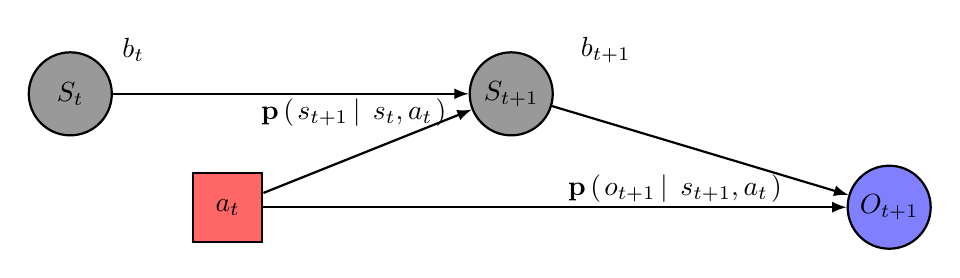
\begin{tikzpicture}[scale=0.8]
%%%%%%%%%%%%%%%%%%%%%%%%%%%%%%%%%%%%%%%%%%%%%%%%%%%%%%%%%%%%%%
%vertex
\tikzstyle{vertex}=[circle,fill=black!40,minimum size=30pt,inner sep=0pt,draw=black,thick]
\tikzstyle{avertex}=[rectangle,fill=red! 60,minimum size=25pt,inner sep=0pt,draw=black,thick]
\definecolor{darkgreen}{rgb}{0.3,0.8,0.5}
\tikzstyle{overtex}=[circle,fill=blue!50,minimum size=30pt,inner sep=0pt,draw=black,thick]
%nodes
\node[vertex] (state1) at (0,1.8) {$S_t$};
\node[vertex] (state2) at (7,1.8) {$S_{t+1}$};
\node[overtex] (obs) at (13,0) {$O_{t+1}$};
\node[avertex] (action) at (2.5,0) {$a_t$};
%%bels
\node (bel1) at (1,2.5) {$b_t$};
\node (bel2) at (8.5,2.5) {$b_{t+1}$};
%probas
\node (trans) at (4.5,1.5) {$\textbf{p} \paren{ s_{t+1} \sachant s_t, a_t }$};
\node (observ) at (9.6,0.3) {$\textbf{p} \paren{ o_{t+1} \sachant s_{t+1}, a_t }$};
%%%%%%%%%%%%%%%%%%%%%%%%%%%%%%%%%%%%%%%%%%%%%%%%%%%%%%%%%%%%%%
%ARROWS
\draw[->,>=latex, thick] (state1) -- (state2);
\draw[->,>=latex, thick] (state2) -- (obs);
\draw[->,>=latex, thick] (action) -- (state2);
\draw[->,>=latex, thick] (action) -- (obs);
\end{tikzpicture}
\vspace{-0.8cm}
\caption[Bayesian Network illustrating the belief update.]{Bayesian Network illustrating the belief update}
\end{figure}%
\vspace{-0.4cm}
\begin{itemize}
\item { \color{black!40} the \textbf{system states} are the gray circular nodes},
\item { \color{red!60} the \textbf{action} is the red square node }, 
\item and { \color{blue!50} the \textbf{observation} is the blue circular node}.
\end{itemize}
\vspace{0.2cm}
The belief state $b_{t}$ (resp. $b_{t+1}$)
is the probabilistic estimation of the current (resp. next) system state $s_t$ (resp. $s_{t+1}$)
\begin{exampleblock}{\textbf{probabilistic} belief update}
\begin{center}
$ b_{t+1}(s') %= u(b_t,a,o') 
\propto \textbf{p} \paren{ o' \sachant s',a} \cdot \sum_{s \in \mathcal{S}} \textbf{p} \paren{ s' \sachant s,a} \cdot b_t(s)  $
\end{center}
\end{exampleblock}
\end{frame}

\begin{frame}
\frametitle{Rewritings of parameters}
\framesubtitle{\footnotesize \textbf{PROBABILISTIC} parameters}
\begin{itemize}
\item $T^a_j \paren{ \mathbb{S},s_j' } = T^a_j \paren{\mathcal{P}(s_j'),s_j'}$;
\item $O^a_i \paren{ \mathbb{S}',o_i' } = O^a_i \paren{\mathcal{P}(o_i'),o_i'}$.
\end{itemize}
\visible<2->{
\begin{block}{consequences on the joint distribution}
\vspace{-0.3cm}
\begin{align*}
\textbf{p} \paren{ o_i', \mathcal{P}(o_i') \sachant \mathbb{S}, a} & = O^a_i \paren{ \mathcal{P}(o_i'), o_i'} \cdot \displaystyle \prod_{s_j'\in\mathcal{P}(o_i')} T^a_i \paren{\mathcal{P}(s_j'),s_j'} \\
& = \textbf{p} \paren{ o_i', \mathcal{P}(o_i') \sachant \mathcal{Q}(o_i'), a}.
\end{align*}
\end{block}
}
\visible<3->{
\vspace{-0.2cm}
\begin{alertblock}{observation probabilities}
epistemic state % sur $\mathbb{S}$: $b^{\pi} \in \Pi_{S}$.
\vspace{-0.7cm}
\begin{equation*}
 b^{\pi}(\mathbb{S}) \xrightarrow{ \mbox{\footnotesize \textbf{marginalization}} }  b^{\pi}(\mathcal{Q}(o_i')) \xrightarrow{ \begin{array}{cc} \mbox{\footnotesize \textbf{pignistic}}
\vspace{-0.2cm}
\\
 \mbox{\footnotesize \textbf{transformation}} \end{array} } \overline{b^{\pi}}(\mathcal{Q}(o_i')) 
\end{equation*} 
\vspace{-0.5cm}
\[ { \color{red} \textbf{p} \paren{ o_i' \sachant b^{\pi}, a } } = \sum_{2^{\mathcal{P}(o_i')},2^{\mathcal{Q}(o_i')}} \textbf{p} \paren{ o_i', \mathcal{P}(o_i') \sachant \mathcal{Q}(o_i'), a} \cdot \overline{b^{\pi}}(\mathcal{Q}(o_i')) \]
\end{alertblock}
}
\end{frame}
\begin{frame}
\frametitle{Parameters rewritings}
\framesubtitle{\footnotesize \textbf{POSSIBILISTIC} parameters}
\begin{itemize}
\item $\pi \paren{ s_j' \sachant \mathbb{S}, a } = \pi \paren{s_j' \sachant \mathcal{P}(s_j'), a}$;
\item $\pi \paren{ o_i' \sachant \mathbb{S}', a } = \pi \paren{o_i' \sachant \mathcal{P}(o_i'), a}$.
\end{itemize}
\visible<2->{
\begin{alertblock}{marginal possibilistic belief states}
$\forall o_i' \in \mathbb{O}$,\\
$ \displaystyle b^{\pi}_{t+1} \Big( \hspace{-0.05cm} \mathcal{P}(o_i') \hspace{-0.05cm} \Big) \propto^{\pi}  \pi  \Big( o_i', \mathcal{P}(o_i') \Big\vert a_0,o_1, \ldots, a_{t-1}, o_{t} \Big)$ \\
\visible<3->{
\hspace{2.93cm} $\displaystyle = \max_{2^{\mathcal{Q}(o_i')}} \hspace{-0.05cm} \min \hspace{-0.07cm} \Bigg\{ \hspace{-0.07cm} \pi \hspace{-0.05cm} \Big( \hspace{-0.05cm} o_i', \hspace{-0.05cm} \mathcal{P}(o_i') \hspace{-0.02cm} \Big\vert \hspace{-0.02cm} \mathcal{Q}(o_i'), \hspace{-0.05cm} a \hspace{-0.05cm} \Big)\hspace{-0.05cm}, \hspace{-0.05cm} b^{\pi}_t \hspace{-0.05cm} \Big( \hspace{-0.05cm} \mathcal{Q}(o_i') \hspace{-0.05cm} \Big) \hspace{-0.1cm} \Bigg\}$\\
}
\visible<4->{
\hspace{5cm} denoted by { \color{red} $\pi \Big( o_i', \mathcal{P}(o_i') \Big\vert b^{\pi}_t, a \Big)$}.
}
\end{alertblock}
}
\end{frame}

\begin{frame}
\definecolor{bblue}{rgb}{0,0.4,0.75}
\frametitle{A possibilistic belief state}
\framesubtitle{\footnotesize finite belief space}
\vspace{0.2cm}
$\Pi^{\mathcal{L}}_{\mathcal{S}} = \Big\{$ possibility distributions $\Big\}$: $\# \Pi^{\mathcal{L}}_{\mathcal{S}} < + \infty$\\ 
\vspace{0.1cm} 
$\rightarrow $ \textbf{finite belief space}
\vspace{-0.1cm}
\visible<2->{
\[ { \color{bblue}  b^{\pi}_{t} (s) = \pi \paren{ s_t = s \sachant a_0,o_1, \ldots, a_{t-1}, o_t } } \]
}
\vspace{-0.6cm}
\visible<3->{
\begin{exampleblock}{update -- \textbf{possibilistic} belief state}
\vspace{0.1cm}
$b^{\pi}_{t+1}(s')  %= u(b^{\pi}_{t},a,o')(s') 
=  \left \{ \begin{array}{ccc} 1 & \hspace{-1cm} \mbox{ if } \pi \paren{ o',s' \sachant b_t^{\pi}, a} = \pi \paren{ o' \sachant b_t^{\pi}, a} \\
\pi \paren{ o', s' \sachant b_t^{\pi}, a} & \mbox{ otherwise.}  
\end{array} \right.$ \\
\vspace{0.3cm}
${ \color{red} \mbox{ denoted by } }  { b^{\pi}_{t+1}(s') \color{red} \propto^{\pi} \pi \paren{o',s'\sachant b_t^{\pi}, a}} $
\end{exampleblock}
}
\visible<4>{
\begin{itemize}
\item $\displaystyle  \pi ( o', s' \vert b_t^{\pi}, a)  = \max_{s \in \mathcal{S}} \min \Big\{ \pi ( o' \vert s', a ), \pi ( s' \vert s, a ), b^{\pi}_t(s) \Big\}$;
\item $ \displaystyle \pi \paren{o' \sachant s', a} = \max_{s' \in \mathcal{S} } \pi \paren{ o',s' \sachant b^{\pi}_t, a  }$.
\end{itemize}
}
\vspace{-0.2cm}
\visible<5->{
\begin{block}{}
\begin{itemize}
\item the update \textbf{only depends on $o'$ and $a$}.
\end{itemize}
\end{block}
}
\end{frame}


\begin{frame}
\begin{block}{Dynamic Programming scheme: $\#$ iterations $<\# \mathcal{X}$.}
$\forall x \in \mathcal{X}$, $V_0(x) = \rho(x)$ \textbf{preference}, 
\visible<2->{
and, until convergence,
$\bullet V_{i+1}(x) = \displaystyle \max_{a \in \mathcal{A}} \max_{x' \in \mathcal{X}} \min \set{ \pi \paren{ x' \sachant x , a} , V_i(x') }$,}
\visible<3->{
 \mbox{ and } \\
$\mbox{if } V_{i+1}(x) \hspace{-0.1cm} > \hspace{-0.1cm} V_i(x), \delta(x) \hspace{-0.1cm} = \hspace{-0.1cm} \displaystyle \operatorname*{argmax}_{a \in \mathcal{A}} \hspace{-0.05cm} \max_{x' \in \mathcal{X}} \hspace{-0.05cm} \min \hspace{-0.1cm} \set{ \hspace{-0.1cm} \pi \paren{ x' \sachant x , a} , \hspace{-0.1cm} V_i(x') \hspace{-0.1cm} }$.}
\end{block}
\end{frame}

\begin{frame}
\frametitle{Resulting $\pi$-MOMDP solver: PPUDD}
\centering
\begin{block}{}
\begin{itemize}
\item probabilistic model: $+$ and $\times$ $\Rightarrow$ new values created, \\ 
number of ADDs leaves \textbf{potentially huge}.
\item possibilistic model: $\min$ and $\max$ $\Rightarrow$ values $\in \mathcal{L}$ finite, 
number of leaves bounded, \textbf{ ADDs \textbf{smaller}}.
\end{itemize}
\end{block}
\vspace{-0.6cm}
\begin{figure}
\begin{tikzpicture}
		\visible<2->{
	\node (PPUDD) at (2.5,15) {\textbf{PPUDD: Possibilistic Planning Using Decision Diagrams}};
	
	\node (algo) at (0,12.7) {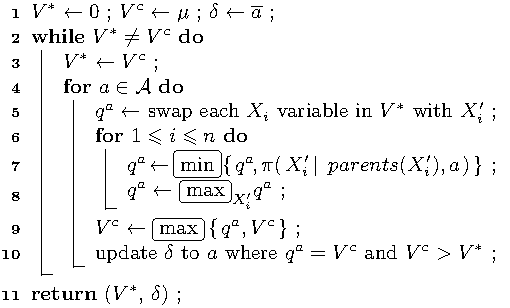
\includegraphics[scale=0.75]{algo2.pdf}};
}	
	\visible<3->{	
	\node (blabla1) at (5.7,14.2) {factorization};
	\node (blabla12) at (5.7,13.6) {{\color{blue!80} $\Rightarrow$ dynamic programming}};
	\draw[ultra thick,>=latex,->,blue!80] (3.7,13.8) to (-0.5,14.2);
	}	
	\visible<4->{
	\node (blabla13) at (5.9,13.1) {{\color{orange} divided into $n$ stages}};
	\node (blabla15) at (5.5,12) {{\color{red} used ADDs smaller}};
	\node (blabla16) at (5.7,11.5) {{\color{red} $\rightarrow$ \textbf{faster computations.}}};
	\draw[ultra thick,>=latex,->,orange] (3.6,13.1) to (0,12.9);	
	\node (accolade) at (-2.35,12.5) {\resizebox{0.93cm}{!}{{ \color{orange} $\{$}}}; 
}
\end{tikzpicture}
\end{figure}
\visible<2->{
\vspace{-0.4cm}
computations on trees: \textit{CU Decision Diagram Package}.
}
\end{frame}

\begin{frame}
\frametitle{Pignistic transformation and transitions}
\framesubtitle{\footnotesize Pignistic transformation}
numbering of the $n = \# \mathcal{S}$ system states:
$1 = b^{\pi}(s_1) \geqslant \ldots \geqslant b^{\pi}(s_{n}) \geqslant b^{\pi}(s_{n+1}) = 0$.
\begin{exampleblock}{\textbf{pignistic transformation} -- $P: \Pi_{\mathcal{S}} \rightarrow \mathbb{P}_{S} $}
\[ \overline{b^{\pi}}(s_i) = \sum_{j=i}^{\# \mathcal{S}} \frac{b^{\pi}(s_j) - b^{\pi}(s_{j+1})}{j}.\]
\end{exampleblock}
\begin{itemize}
\item probability distribution $\overline{b^{\pi}}$ $=$ \textbf{gravity center} \\ 
\hspace{1cm} of the represented probabilistic distributions;
%induites par la distribution de possibilité $b^{\pi}$ 
\item \textbf{Laplace principle}: ignorance $\rightarrow$ uniform probability.
\end{itemize}
%\begin{tikzpicture} 
%\draw [domain=-7:-1] plot(\x,0);
%\draw [domain=-2:2, scale=0.6] plot (\x-7.5,{exp(-\x*\x)});
%\draw [domain=-2:3, scale=0.6] plot (\x-7.5,{0.5*exp(-\x*(\x-2))});
%\node (poss) at (-3,0.5) {$\pi$};
%\node (pref) at (-5.5,0.5) {$\mu$};
%\node (S) at (-7.5,0) {$S$};
%\draw [domain=-2:2] plot(\x,0);
%\draw [domain=-1:0.35, scale=0.6, color=red] plot (\x-1,{0.5*exp(-\x*(\x-2))});
%\draw [domain=0.35:2, scale=0.6, color=red] plot (\x-1,{exp(-\x*\x)});
%\draw [domain=-2:0.35, scale=0.6, color=blue] plot (\x-1,{exp(-\x*\x)});
%\draw [domain=0.35:3, scale=0.6, color=blue] plot (\x-1,{0.5*exp(-\x*(\x-2))});
%\node [color=red] (inter) at (-0.5,-0.2) {$f_{\textbf{P} \cap \textbf{M}}$};
%\node [color=blue] (union) at (-1.5,0.7) {$f_{\textbf{P} \cup \textbf{M}}$};
%\end{tikzpicture}
\end{frame}

\begin{frame}
\frametitle{Pignistic transformation}
\framesubtitle{\footnotesize Examples of pignistic transformations (red) of possibility distributions (blue)}
\begin{tikzpicture}[scale=0.55,transform shape]
\begin{axis}[ymax=1.4,grid=major,xlabel={states},legend entries={possibility, pignistic probability}]
\addplot [ybar, bar width = 30pt,draw=blue,fill=blue, ultra thick] table[x=index,y=possib] {pignistique/plot1.txt};
\addplot [ybar, draw=red, fill=red, ultra thick] table[x=index,y=proba] {pignistique/plot1.txt};
\end{axis}
\end{tikzpicture}
\hspace{0.8cm}
\begin{tikzpicture}[scale=0.55,transform shape]
\begin{axis}[ymax=1.4,grid=major,xlabel={states},legend entries={possibility, pignistic probability}]
\addplot [ybar, bar width = 30pt,draw=blue,fill=blue, ultra thick] table[x=index,y=possib] {pignistique/plot2.txt};
\addplot [ybar, draw=red, fill=red, ultra thick] table[x=index,y=proba] {pignistique/plot2.txt};
\end{axis}
\end{tikzpicture}
\begin{tikzpicture}[scale=0.55,transform shape]
\begin{axis}[ymin=-0.1,ymax=1.4,grid=major,xlabel={states},legend entries={possibility, pignistic probability}]
\addplot [ybar, bar width = 30pt,draw=blue,fill=blue, ultra thick] table[x=index,y=possib] {pignistique/plot3.txt};
\addplot [ybar, draw=red, fill=red, ultra thick] table[x=index,y=proba] {pignistique/plot3.txt};
\end{axis}
\end{tikzpicture}
\hspace{0.8cm}
\begin{tikzpicture}[scale=0.55,transform shape]
\begin{axis}[ymax=1.4,grid=major,xlabel={states},legend entries={possibility, pignistic probability}]
\addplot [ybar, bar width = 30pt,draw=blue,fill=blue, ultra thick] table[x=index,y=possib] {pignistique/plot4.txt};
\addplot [ybar, draw=red, fill=red, ultra thick] table[x=index,y=proba] {pignistique/plot4.txt};
\end{axis}
\end{tikzpicture}

\end{frame}


\begin{frame}
\frametitle{hybrid POMDP and $\pi$-POMDP}
\framesubtitle{\footnotesize differences with possibilistic models}
\begin{tabular}{|c||c|c|}
  \hline
  & hybrid POMDP  & $\pi$-POMDP \\
  \hline \hline
\hspace{-0.2cm} transitions \hspace{-0.2cm} & probabilities & qualitative possibility \\
  \hline
\hspace{-0.2cm} rewards \hspace{-0.2cm} & quantitative $\in \mathbb{R}$ & qualitative $\in \mathcal{L}$  \\
  \hline
\hspace{-0.2cm} situation \hspace{-0.2cm} & 
\begin{tabular}{c} -some imprecisions \\ -large POMDP \end{tabular} & few quantitative \\
  \hline
\hspace{-0.2cm} issues & $\pi$ definition & commensurability \\
  \hline
in practice & MDP & $\pi$-MDP\\
\hline
\end{tabular}
\\
\vspace{0.3cm}
\visible<2->{
\textbf{hybrid model:}
\begin{itemize}
\item only belief states are possibilistic:
\end{itemize}
$\rightarrow$ agent knowledge $=$ \textbf{possibility} distribution;
\begin{itemize}
\item probabilistic dynamics:
\end{itemize}
$\rightarrow$ \textbf{approximated} (prob.) transition between epistemic states. 
}
\end{frame}

%\section{Benefiting from factorized structures}
\begin{frame}
\frametitle{factorized POMDP}
\framesubtitle{\footnotesize definition}
\begin{itemize}
\item $\mathcal{S}$ described by $\mathbb{S} = \set{ s_1, \ldots, s_m }$: $\mathcal{S} = s_1 \times \ldots \times s_m$.\\
Notation: $\mathbb{S}' = \set{s_1', \ldots, s_m'}$;
\end{itemize}
\visible<2->{
\begin{itemize}
\item \textbf{transition} function of $s_j'$,\\ 
$T_j^a(\mathbb{S}, s'_j) = \textbf{p} \paren{ s'_j \sachant \mathbb{S}, a}$,
$\forall j \in \set{1, \ldots, m}$ et $\forall a \in \mathcal{A}$;
\end{itemize}
}
\visible<3->{
\begin{itemize}
\item $\mathcal{O}$ described by $\mathbb{O}=\set{ o_1, \ldots, o_n }$: $\mathcal{O} = o_1 \times \ldots \times o_n$;
\end{itemize}
}
\visible<4->{
\begin{itemize}
\item \textbf{observation} function of $o_i'$,\\
$O_i^a(\mathbb{S}', o'_i) = \textbf{p} \paren{ o'_i \sachant \mathbb{S}', a}$,
$\forall i \in \set{1,\ldots,n}$ et $\forall a \in \mathcal{A}$.
\end{itemize}
}
\vspace{0.3cm}
\visible<5->{
\textbf{independences:} \\
\vspace{0.1cm}
$\rightarrow$ $ \forall s_i',s_j' \in \mathbb{S}'$, \hspace{0.55cm} $s_i' \perp\!\!\!\perp s_j' \ \vert \set{\mathbb{S}, a \in \mathcal{A} }$,\\
\vspace{0.3cm}
$\rightarrow$ $\forall o_i', o_j' \in \mathbb{O}'$, \hspace{0.3cm} $o_i' \perp\!\!\!\perp o_j' \ \vert \set{ \mathbb{S}', a \in \mathcal{A} }$.
}
\end{frame}

\begin{frame}
\frametitle{Notations}
\framesubtitle{\footnotesize some variables does not interact with each other}
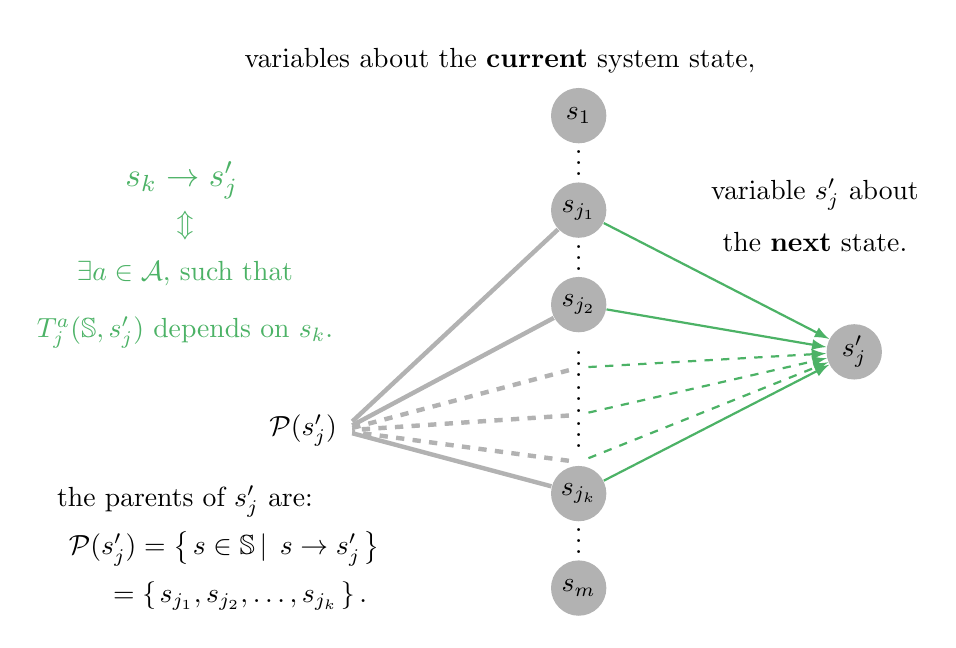
\begin{tikzpicture}
\node (legend0) at (-1,0.5) {};
\node (legend) at (-1,0.2) {variables about the \textbf{current} system state,};
\node (legend2) at (3,-1.5) {variable $s_j'$ about};
\node (legend3) at (3,-2.1) { the \textbf{next} state.};
\begin{scope}[scale=1.2,transform shape]
\visible<2->{
\node (A) at (-4.2,-1.1) { {\color[rgb]{0.3,0.7,0.4} $s_k \rightarrow s_j'$}};
}
\end{scope}

\definecolor{ggreen}{rgb}{0.3,0.7,0.4};
%	\node (legend2) at (-4,-0.6) {$s_k \thickrightarrow s_j'$};
\visible<2->{
\node (legend2) at (-5,-1.9) {{\color{ggreen} $\Updownarrow$}};
\node (legend2) at (-5,-2.5) {{\color{ggreen} $\exists a \in \mathcal{A}$, such that}};
\node (legend2) at (-5,-3.25) {{\color{ggreen} $T^a_j(\mathbb{S},s_j')$ depends on $s_k$.}};
}
%node
\tikzstyle{vertex}=[circle,fill=black!30,minimum size=20pt,inner sep=0pt]
\node[vertex] (s1) at (0,-0.5) {$s_1$};
\node (dots1) at (0,-1) {$\vdots$};
\node[vertex] (sk1) at (0,-1.7) {$s_{j_1}$};
\node (dots2) at (0,-2.2) {$\vdots$};
\node[vertex] (sk2) at (0,-2.9) {$s_{j_2}$};
\node (skF1) at (0,-3.7) {};
\node (skF2) at (0,-4.3) {};
\node (skF3) at (0,-4.9) {};
\node (dots3) at (0,-3.55) {$\vdots$};
\node (dots3) at (0,-4) {$\vdots$};
\node (dots3) at (0,-4.45) {$\vdots$};
\node[vertex] (sk3) at (0,-5.3) {$s_{j_k}$};
\node (dots4) at (0,-5.8) {$\vdots$};
\node[vertex] (sm) at (0,-6.5) {$s_m$};
\node[vertex] (spj) at (3.5,-3.5) {$s_j'$};
\visible<2->{
%draw
\draw[->,>=latex,thick,color=ggreen] (sk1) to (spj);
\draw[->,>=latex,thick,color=ggreen] (sk2) to (spj);
\draw[->,>=latex,thick,dashed,color=ggreen] (skF1) to (spj);
\draw[->,>=latex,thick,dashed,color=ggreen] (skF2) to (spj);
\draw[->,>=latex,thick,dashed,color=ggreen] (skF3) to (spj);
\draw[->,>=latex,thick,color=ggreen] (sk3) to (spj);
}
\visible<3->{
%legend
%\tikzstyle{point}=[circle,fill=black]
\node (nearP) at (-3,-4.5) {};
\draw[ultra thick,color=black!30] (sk1) to (nearP);
\draw[ultra thick,color=black!30] (sk2) to (nearP);
\draw[ultra thick,dashed,color=black!30] (skF1) to (nearP);
\draw[ultra thick,dashed,color=black!30] (skF2) to (nearP);
\draw[ultra thick,dashed,color=black!30] (skF3) to (nearP);
\draw[ultra thick,color=black!30] (sk3) to (nearP);
 
\node (parents) at (-3.5,-4.5) {$\mathcal{P}(s_j')$};
\node (parents2) at (-5,-5.4) {the parents of $s_j'$ are:};
\node (parents2) at (-4.5,-6) {$\mathcal{P}(s_j') = \set{ s \in \mathbb{S} \sachant s \rightarrow s_j'} $};
\node (parents3) at (-4.3,-6.6) {$ = \set{ s_{j_1}, s_{j_2}, \ldots,s_{j_k} }.$};
}
%\begin{scope}[scale=6,transform shape]
%\node (A) at (-0.1,-0.42) {$\{$};
%\end{scope}
\end{tikzpicture}
\end{frame}

\begin{frame}
\vspace{0.25cm}
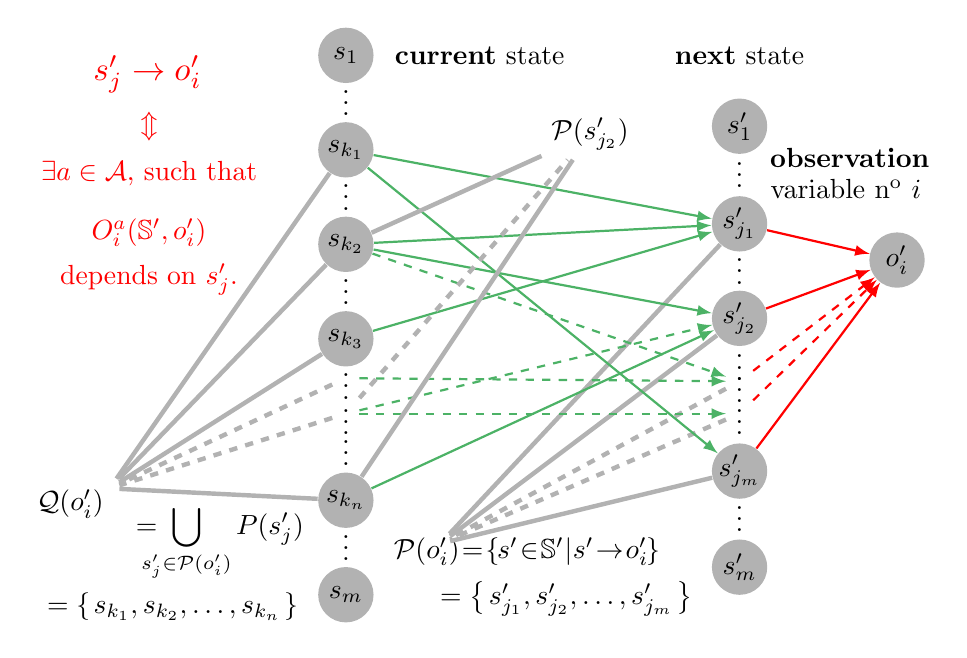
\begin{tikzpicture}
\definecolor{ggreen}{rgb}{0.3,0.7,0.4};
\frametitle{Notations}
\framesubtitle{\footnotesize concerning observation variables}
\visible<2->{
\begin{scope}[scale=1.2,transform shape]
\node (A) at (-2.1,-0.2) { {\color{red} $s_j' \rightarrow o_i'$}};
\end{scope}
\node (legend2) at (-2.5,-0.9) {{\color{red} $\Updownarrow$}};
\node (legend2) at (-2.5,-1.5) {{\color{red} $\exists a \in \mathcal{A}$, such that}};
\node (legend2) at (-2.5,-2.25) {{\color{red} $O^a_i(\mathbb{S}',o_i')$}};
\node (legend2) at (-2.5,-2.85) {{\color{red} depends on $s_j'$.}};
}
\tikzstyle{vertex}=[circle,fill=black!30,minimum size=20pt,inner sep=0pt]
\visible<4->{
\node (led) at (1.7,0) {\textbf{current} state};
\node[vertex] (s1) at (0,0) {$s_1$};
\node (dots1) at (0,-0.5) {$\vdots$};
\node[vertex] (sk1) at (0,-1.2) {$s_{k_1}$};
\node (dots2) at (0,-1.7) {$\vdots$};
\node[vertex] (sk2) at (0,-2.4) {$s_{k_2}$};
\node (dots3) at (0,-2.9) {$\vdots$};
\node[vertex] (sk3) at (0,-3.6) {$s_{k_3}$};
\node (dots4) at (0,-4.1) {$\vdots$};
\node (dots5) at (0,-4.55) {$\vdots$};
\node (dots6) at (0,-4.95) {$\vdots$};
\node[vertex] (sk4) at (0,-5.65) {$s_{k_n}$};
\node (dots7) at (0,-6.15) {$\vdots$};
\node[vertex] (sm) at (0,-6.85) {$s_m$};
}
\node (led) at (5,0) {\textbf{next} state};
\node[vertex] (sp1) at (5,-0.9) {$s_1'$};
\node (dotsp1) at (5,-1.42) {$\vdots$};
\node[vertex] (spj1) at (5,-2.14) {$s'_{j_1}$};
\node (dotsp2) at (5,-2.64) {$\vdots$};
\node[vertex] (spj2) at (5,-3.34) {$s'_{j_2}$};
\node (dotsp3) at (5,-3.86) {$\vdots$};
\node (dotsp5) at (5,-4.14) {$\vdots$};
\node (dotsp6) at (5,-4.55) {$\vdots$};
\node[vertex] (spj3) at (5,-5.28) {$s'_{j_m}$};
\node (dotsp4) at (5,-5.78) {$\vdots$};
\node[vertex] (smp) at (5,-6.5) {$s'_m$};

\visible<3>{
\node (poi) at (2.3,-6.3) {$\mathcal{P}(o_i') \hspace{-0.07cm} = \hspace{-0.07cm} \set{ \hspace{-0.07cm} s' \hspace{-0.07cm} \in \hspace{-0.07cm} \mathbb{S}' \hspace{-0.05cm} \sachant \hspace{-0.15cm} s' \hspace{-0.07cm} \rightarrow \hspace{-0.07cm} o_i' \hspace{-0.07cm}} $};
\node (h2) at (2.8,-6.9) { $= \set{ s'_{j_1}, s'_{j_2}, \ldots, s'_{j_m} }$};

\visible<3>{
\node (nearP) at (1.2,-6.2) {};
\draw[ultra thick,color=black!30] (spj1) to (nearP);
\draw[ultra thick,color=black!30] (spj2) to (nearP);
\draw[ultra thick,color=black!30] (spj3) to (nearP);
\draw[ultra thick,dashed,color=black!30] (dotsp6) to (nearP);
\draw[ultra thick,dashed,color=black!30] (dotsp5) to (nearP);
}
}

\visible<5->{
\draw[->,>=latex,thick,color=ggreen] (sk1) to (spj1);
\draw[->,>=latex,thick,color=ggreen] (sk2) to (spj1);
\draw[->,>=latex,thick,color=ggreen] (sk3) to (spj1);
\draw[->,>=latex,thick,color=ggreen] (sk2) to (spj2);
\draw[->,>=latex,thick,color=ggreen] (sk4) to (spj2);
\draw[->,>=latex,thick,color=ggreen] (sk1) to (spj3);
\draw[->,>=latex,thick,dashed,color=ggreen] (dots4) to (dotsp5);
\draw[->,>=latex,thick,dashed,color=ggreen] (sk2) to (dotsp5);
\draw[->,>=latex,thick,dashed,color=ggreen] (dots5) to (dotsp6);
\draw[->,>=latex,thick,dashed,color=ggreen] (dots5) to (spj2);
}
\visible<-2>{
\node (o) at (6.4,-1.3) {\textbf{observation}};
\node (o) at (6.35,-1.7) {variable n\textsuperscript{o} $i$};
}
\node[vertex] (opi) at (7,-2.6) {$o'_{i}$};
\visible<2->{
\draw[->,>=latex,thick,color=red] (spj1) to (opi);
\draw[->,>=latex,thick,color=red] (spj2) to (opi);
\draw[->,>=latex,thick,color=red] (spj3) to (opi);
\draw[->,>=latex,thick,dashed,color=red] (dotsp5) to (opi);
\draw[->,>=latex,thick,dashed,color=red] (dotsp6) to (opi);
}
\visible<6>{
\node (nearPS) at (3.1,-1) {$\mathcal{P}(s_{j_2}')$};
\draw[ultra thick,color=black!30] (sk2) to (nearPS);
\draw[ultra thick,color=black!30] (sk4) to (nearPS);
\draw[ultra thick,dashed,color=black!30] (dots5) to (nearPS);
}

\visible<7->{
\node (parents) at (-3.5,-5.7) {$\mathcal{Q}(o_i')$}; 
\node (parents) at (-1.6,-6.2) {$ =\hspace{-0.3cm} \displaystyle \bigcup_{s_j' \in \mathcal{P}(o_i')} P(s_j')$}; 
\node (parents) at (-2.2,-7) {$ = \set{ s_{k_1},s_{k_2},\ldots,s_{k_n} }$};

\node (nearQ) at (-3,-5.5) {};
\draw[ultra thick,color=black!30] (sk1) to (nearQ);
\draw[ultra thick,color=black!30] (sk2) to (nearQ);
\draw[ultra thick,color=black!30] (sk3) to (nearQ);
\draw[ultra thick,dashed,color=black!30] (dots4) to (nearQ);
\draw[ultra thick,dashed,color=black!30] (dots5) to (nearQ);
\draw[ultra thick,color=black!30] (sk4) to (nearQ);
}
\end{tikzpicture}
\end{frame}

\begin{frame}
\definecolor{violet}{rgb}{0.7,0.1,0.5}
\definecolor{orangee}{rgb}{1,0.7,0.1}
\definecolor{gggreen}{rgb}{0,0.7,0.7}
\frametitle{Variables de croyance}
\framesubtitle{\footnotesize different according to the class of the variable}
\definecolor{bblue}{rgb}{0,0.4,0.75}
$\lambda=\# \mathcal{L}$
\visible<2->{
\begin{alertblock}{}
\begin{itemize}
\item {\color{violet} $\forall s'_{v} \in \mathbb{S}_v$, $1$} variable {\color{violet} $\beta'_{v}$} is enough.
\vspace{0.7cm}
\visible<3->{
\item $p_i = \# \mathcal{P}(o_i')$. \\ 
\vspace{0.4cm}
{ \color{gggreen} $ \forall o_i \in \mathbb{O} \setminus \mathbb{S}_v$,}
$\lambda^{2^{p_i}} - (\lambda-1)^{2^{p_i}}$ belief states,\\ 
\vspace{0.3cm}
$\Rightarrow { \color{gggreen} \lceil \log_2(\lambda^{2^{p_i}} - (\lambda-1)^{2^{p_i}}) \rceil}$ boolean variables {\color{gggreen} $\beta_h'$ }.
}
%$\tilde{b}'(\mathcal{P}(o_i')) = \max_{v \in 2^{\mathcal{Q}(o_i')}} \min \set{ \pi \paren{ o_i', \mathcal{P}(o_i') \sachant v,a}, b(v) }$;
\vspace{0.7cm}
\visible<4->{
\item  { \color{orangee} $\forall s'_{f} \in \mathbb{S}_f$,} $\lambda^2 - (\lambda-1)^2 = 2\lambda-1$ belief states,\\ 
\vspace{0.2cm}
$\Rightarrow { \color{orangee} \lceil \log_2(2\lambda-1) \rceil }$ boolean variables {\color{orangee} $\beta_f'$}.
}
\end{itemize}
%where $\pi \paren{ o_i', \mathcal{P}(o'_i) \sachant \mathcal{Q}(o'_i), a }$ 
%$ = \min \set{ \pi \paren{ o_i' \sachant \mathcal{P}(o'_i), a}, \min_{s'_j \in \mathcal{P}(o'_i)} \pi \paren{ s'_j \sachant \mathcal{P}(s'_j), a  } }$.
\end{alertblock}
}
\end{frame}

\begin{frame}
\definecolor{violet}{rgb}{0.7,0.1,0.5}
\definecolor{orangee}{rgb}{1,0.7,0.1}
\definecolor{gggreen}{rgb}{0,0.7,0.7}
\frametitle{resulting MDP in practice}
\framesubtitle{\footnotesize final structured MDP }
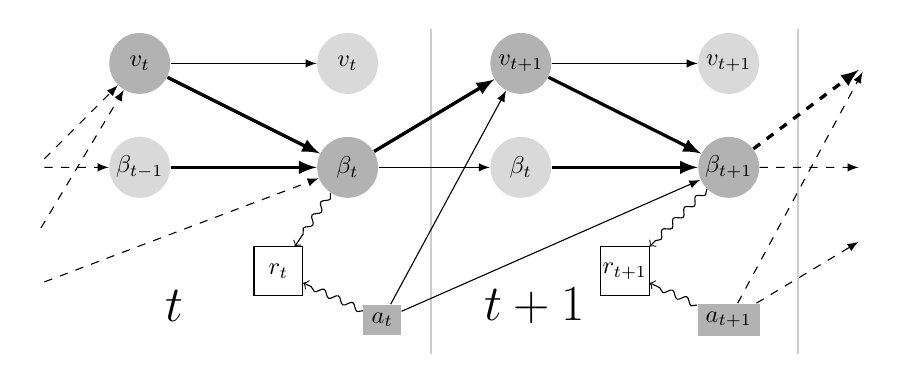
\begin{tikzpicture}[scale=0.88,transform shape]
%%%%%%%%%%%%%%%%%%%%%%%%%%%%%%%%%%%%%%%%%%%%%%%%%%%%%%%%%%%%%%
%TIME/BACKGROUND
\coordinate (middleTop) at (5.7,3);
\coordinate (middleBot) at (5.7,-1.7);
\draw[thick,color=black!20] (middleTop) -- (middleBot);
\node [font=\huge] (statet) at (2,-1) {$t$};
\coordinate (middleTop2) at (11,3);
\coordinate (middleBot2) at (11,-1.7);
\draw[thick,color=black!20] (middleTop2) -- (middleBot2);
\node [font=\huge] (statetplus1) at (7.2,-1) {$t+1$};

%%%%%%%%%%%%%%%%%%%%%%%%%%%%%%%%%%%%%%%%%%%%%%%%%%%%%%%%%%%%%%
%vertex
%vars
\tikzstyle{vertex}=[circle,fill=black!30,minimum size=25pt,inner sep=0pt]
\tikzstyle{vertex2}=[circle,fill=black!15,minimum size=25pt,inner sep=0pt]
\tikzstyle{vertex3}=[ draw, inner sep=0pt, minimum size=20pt]

%1
\node[vertex] (state1) at (1.5,2.5) {$v_t$};
\node[vertex2] (state12) at (1.5,1) {$\beta_{t-1}$};
%1bis
\node[vertex2] (state1bis) at (4.5,2.5) {$v_t$};
\node[vertex] (state12bis) at (4.5,1) {$\beta_t$};
%R1
\node[vertex3] (R1) at (3.5,-0.5) {$r_t$};

%2
\node[vertex] (state2) at (7,2.5) {$v_{t+1}$};
\node[vertex2] (state22) at (7,1) {$\beta_{t}$};

%2bis
\node[vertex2] (state2bis) at (10,2.5) {$v_{t+1}$};
\node[vertex] (state22bis) at (10,1) {$\beta_{t+1}$};
%R2
\node[vertex3] (R2) at (8.5,-0.5) {$r_{t+1}$};

%0
\node (state02) at (0,1) {};
\node (state03) at (0,2) {};
%3
\node (state3) at (12,2.5) {};
\node (state33) at (12,2) {};
\node (state32) at (12,1) {};
\node (state32bis) at (12,0) {};

%action
\node[fill=black!30] (action) at (5,-1.2) {$a_t$};
\node (action0) at (0,0) {};
\node (action02) at (0,-0.7) {};
\node[fill=black!30] (action3) at (10,-1.2) {$a_{t+1}$};

%%%%%%%%%%%%%%%%%%%%%%%%%%%%%%%%%%%%%%%%%%%%%%%%%%%%%%%%%%%%%%
%ARROWS
%1->2
\draw[->,>=latex] (state1) -- (state1bis);
\draw[->,>=latex,very thick] (state1) -- (state12bis);
\draw[->,>=latex, very thick] (state12) -- (state12bis);
%1->2bis
\draw[->,>=latex, very thick] (state12bis) -- (state2);
\draw[->,>=latex] (state12bis) -- (state22);
%0->1
\draw[->,>=latex,dashed] (state02) -- (state1);
\draw[->,>=latex,dashed] (state02) -- (state12);
%2->3
\draw[->,>=latex] (state2) -- (state2bis);
\draw[->,>=latex, very thick] (state2) -- (state22bis);
\draw[->,>=latex, very thick] (state22) -- (state22bis);
%2->3bis
\draw[->,>=latex,dashed, very thick] (state22bis) -- (state3);
\draw[->,>=latex,dashed] (state22bis) -- (state32);

%action
%1
\draw[->,>=latex] (action) -- (state2);
\draw[->,>=latex] (action) -- (state22bis);
\draw[->,decorate,decoration={snake,amplitude=.4mm,segment length=2mm,post length=1mm}] (action) -- (R1); 
%0
\draw[->,>=latex,dashed] (action0) -- (state1);
\draw[->,>=latex,dashed] (action02) -- (state12bis);
%3
\draw[->,>=latex,dashed] (action3) -- (state3);
\draw[->,>=latex,dashed] (action3) -- (state32bis);
\draw[->,decorate,decoration={snake,amplitude=.4mm,segment length=2mm,post length=1mm}] (action3) -- (R2); 

% R
\draw[->,decorate,decoration={snake,amplitude=.4mm,segment length=2mm,post length=1mm}] (state12bis) -- (R1); 
\draw[->,decorate,decoration={snake,amplitude=.4mm,segment length=2mm,post length=1mm}] (state22bis) -- (R2); 
\end{tikzpicture}
\definecolor{violet}{rgb}{0.7,0.1,0.5}
\definecolor{orangee}{rgb}{1,0.7,0.1}
\definecolor{gggreen}{rgb}{0,0.7,0.7}
%$\# \mathbb{S} \cdot \log_2 \paren{ n^{2} } \ll \log_2 \paren{ n^{\# \mathcal{S}} } $
$\#$ \textbf{factorized model}'s variables: $ \# \mathbb{O} \hspace{-0.01cm} + \hspace{-0.01cm} {\color{violet}\#\mathbb{S}_v} +$\\
$\hspace{0.5cm} \displaystyle + {\color{gggreen}\sum_{i=1}^{\# \mathbb{O}_h} \Big\lceil \log_2 \big( \lambda^{2^{p_i}} - (\lambda-1)^{2^{p_i}} \big) \Big\rceil} + {\color{orangee} \# \mathbb{S}_f \cdot \Big\lceil \log_2 \paren{ 2\lambda-1 } \Big\rceil}$ \\
\vspace{0.2cm}
\hspace{0.2cm} { \color{red} $\ll$} \hspace{0.7cm} $\#$ \textbf{initial hybrid model}'s variables: \\
\hspace{5.1cm} $\Big\lceil \log_2 \big( \lambda^{ 2^{\# \mathbb{S}} } - (\lambda-1)^{ 2^{\# \mathbb{S}} } \big) \Big\rceil$\\
\end{frame}

\begin{frame}
\definecolor{violet}{rgb}{0.7,0.1,0.5}
\definecolor{orangee}{rgb}{1,0.7,0.1}
\definecolor{gggreen}{rgb}{0,0.7,0.7}
\frametitle{resulting MDP in practice}
\framesubtitle{\footnotesize final structured MDP}
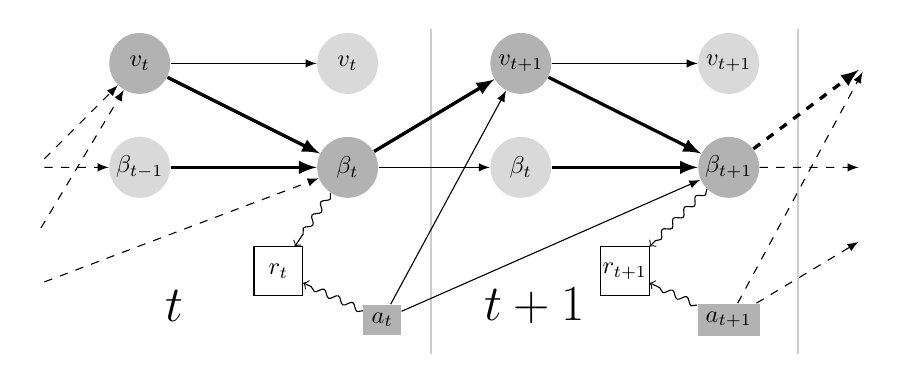
\begin{tikzpicture}[scale=0.88,transform shape]
%%%%%%%%%%%%%%%%%%%%%%%%%%%%%%%%%%%%%%%%%%%%%%%%%%%%%%%%%%%%%%
%TIME/BACKGROUND
\coordinate (middleTop) at (5.7,3);
\coordinate (middleBot) at (5.7,-1.7);
\draw[thick,color=black!20] (middleTop) -- (middleBot);
\node [font=\huge] (statet) at (2,-1) {$t$};
\coordinate (middleTop2) at (11,3);
\coordinate (middleBot2) at (11,-1.7);
\draw[thick,color=black!20] (middleTop2) -- (middleBot2);
\node [font=\huge] (statetplus1) at (7.2,-1) {$t+1$};

%%%%%%%%%%%%%%%%%%%%%%%%%%%%%%%%%%%%%%%%%%%%%%%%%%%%%%%%%%%%%%
%vertex
%vars
\tikzstyle{vertex}=[circle,fill=black!30,minimum size=25pt,inner sep=0pt]
\tikzstyle{vertex2}=[circle,fill=black!15,minimum size=25pt,inner sep=0pt]
\tikzstyle{vertex3}=[ draw, inner sep=0pt, minimum size=20pt]

%1
\node[vertex] (state1) at (1.5,2.5) {$v_t$};
\node[vertex2] (state12) at (1.5,1) {$\beta_{t-1}$};
%1bis
\node[vertex2] (state1bis) at (4.5,2.5) {$v_t$};
\node[vertex] (state12bis) at (4.5,1) {$\beta_t$};
%R1
\node[vertex3] (R1) at (3.5,-0.5) {$r_t$};

%2
\node[vertex] (state2) at (7,2.5) {$v_{t+1}$};
\node[vertex2] (state22) at (7,1) {$\beta_{t}$};

%2bis
\node[vertex2] (state2bis) at (10,2.5) {$v_{t+1}$};
\node[vertex] (state22bis) at (10,1) {$\beta_{t+1}$};
%R2
\node[vertex3] (R2) at (8.5,-0.5) {$r_{t+1}$};

%0
\node (state02) at (0,1) {};
\node (state03) at (0,2) {};
%3
\node (state3) at (12,2.5) {};
\node (state33) at (12,2) {};
\node (state32) at (12,1) {};
\node (state32bis) at (12,0) {};

%action
\node[fill=black!30] (action) at (5,-1.2) {$a_t$};
\node (action0) at (0,0) {};
\node (action02) at (0,-0.7) {};
\node[fill=black!30] (action3) at (10,-1.2) {$a_{t+1}$};

%%%%%%%%%%%%%%%%%%%%%%%%%%%%%%%%%%%%%%%%%%%%%%%%%%%%%%%%%%%%%%
%ARROWS
%1->2
\draw[->,>=latex] (state1) -- (state1bis);
\draw[->,>=latex,very thick] (state1) -- (state12bis);
\draw[->,>=latex, very thick] (state12) -- (state12bis);
%1->2bis
\draw[->,>=latex, very thick] (state12bis) -- (state2);
\draw[->,>=latex] (state12bis) -- (state22);
%0->1
\draw[->,>=latex,dashed] (state02) -- (state1);
\draw[->,>=latex,dashed] (state02) -- (state12);
%2->3
\draw[->,>=latex] (state2) -- (state2bis);
\draw[->,>=latex, very thick] (state2) -- (state22bis);
\draw[->,>=latex, very thick] (state22) -- (state22bis);
%2->3bis
\draw[->,>=latex,dashed, very thick] (state22bis) -- (state3);
\draw[->,>=latex,dashed] (state22bis) -- (state32);

%action
%1
\draw[->,>=latex] (action) -- (state2);
\draw[->,>=latex] (action) -- (state22bis);
\draw[->,decorate,decoration={snake,amplitude=.4mm,segment length=2mm,post length=1mm}] (action) -- (R1); 
%0
\draw[->,>=latex,dashed] (action0) -- (state1);
\draw[->,>=latex,dashed] (action02) -- (state12bis);
%3
\draw[->,>=latex,dashed] (action3) -- (state3);
\draw[->,>=latex,dashed] (action3) -- (state32bis);
\draw[->,decorate,decoration={snake,amplitude=.4mm,segment length=2mm,post length=1mm}] (action3) -- (R2); 

% R
\draw[->,decorate,decoration={snake,amplitude=.4mm,segment length=2mm,post length=1mm}] (state12bis) -- (R1); 
\draw[->,decorate,decoration={snake,amplitude=.4mm,segment length=2mm,post length=1mm}] (state22bis) -- (R2); 
\end{tikzpicture}
\definecolor{violet}{rgb}{0.7,0.1,0.5}
\definecolor{orangee}{rgb}{1,0.7,0.1}
\definecolor{gggreen}{rgb}{0,0.7,0.7}
%$\# \mathbb{S} \cdot \log_2 \paren{ n^{2} } \ll \log_2 \paren{ n^{\# \mathcal{S}} } $
$\#$ \textbf{factorized model}'s variables:\\
\hspace{1cm} $ \leqslant \displaystyle \# \mathbb{O} + { \color{violet} \# \mathbb{S}_v} + { \color{gggreen} \sum_{i=1}^{\# \mathbb{O}_h} \log_2 (\lambda) \cdot 2^{p_i} } + { \color{orangee} \# \mathbb{S}_f \cdot (1 + \log_2(\lambda)) } $ \\
\vspace{0.3cm}
\hspace{0.2cm} { \color{red} $\ll$} \hspace{0.7cm} $\#$ \textbf{initial hybrid model}'s variables: \\
\hspace{5.1cm} $\geqslant \log_2(\lambda) \cdot (2^{\# \mathbb{S}}-1)$.
\end{frame}

\begin{frame}
\frametitle{Variable classification}
\framesubtitle{\footnotesize $3$ classes of state variables -- state space factorization}%: extension des MOMDPs (Araya-L\'opez, Ong)}
\vspace{0.1cm}
\begin{tikzpicture}
\definecolor{violet}{rgb}{0.7,0.1,0.5};
\definecolor{orangee}{rgb}{1,0.7,0.1};
\definecolor{gggreen}{rgb}{0,0.7,0.7};
% separations
\node (T1) at (-1.5,8.4) {};
\node (B1) at (9,8.4) {};
\draw[thick,dashed,color=black!30] (B1) to (T1);
\node (T2) at (-1.5,5.1) {};
\node (B2) at (9,5.1) {};
\draw[thick,color=black!30] (B2) to (T2);

% variables
\tikzstyle{vertex}=[circle,fill=black!30,minimum size=20pt,inner sep=0pt]
\node (V) at (1,10) { \underline{variable:} \color{violet} visible $s_v' \in \mathbb{S}_v$ };
\node[vertex] (vv) at (6.5,9.7) {$s_v'$};
\node (IHV) at (1.3,8) { {\color{gggreen} inferred hidden $ s_h' \in \mathbb{S}_h$} };
\node[vertex] (ihv) at (6.5, 7.15) {$s_h'$};
\node (FHV) at (2,4.75) { {\color{orangee} fully hidden $s_f' \in \mathbb{S}_f$}};
\node[vertex] (fhv) at (6.5,4) {$s_f'$};

\visible<2->{
% visible
\node[vertex] (ov) at (8.5,9.7) {$o_v'$};
\draw[->,>=latex,thick] (vv) to (ov);
\node at (7.5,10) {$s_v'= o_v'$};
}
\visible<3->{
\node (leg1) at (3.5,8.9) {  \color{violet} $\textbf{p} \paren{ s_v' \sachant b_t^{\pi},a } = \sum_{2^{\mathcal{P}(s_v')}} T^a \hspace{-0.04cm} \paren{ \mathcal{P}(s_v'), s_v'} \cdot \overline{b^{\pi}_t} \Big(\mathcal{P}(s_v') \Big)$ };
}
\visible<4->{
\node (leg1) at (2,9.5) { $\Leftrightarrow$ deterministic belief variable. };
}

\visible<5->{
% inférée
\tikzstyle{hvertex}=[circle,fill=black!10,minimum size=20pt,inner sep=0pt]
\node[vertex] (oh) at (8.5,7.15) {$o_i'$};
\draw[->,>=latex,thick] (ihv) to (oh);
\node[hvertex] (sh1) at (6.5,8) {$s_h^{a}$};
\node[hvertex] (sh2) at (6.8,6.2) {$s_h^{b}$};
\node[hvertex] (sh3) at (7.5,5.5) {$s_h^{c}$};
\draw[->,>=latex,thick,dashed] (sh1) to (oh);
\draw[->,>=latex,thick,dashed] (sh2) to (oh);
\draw[->,>=latex,thick,dashed] (sh3) to (oh);
}

\visible<6->{
\node (leg2) at (2,7.3) {$ {\color{gggreen} b^{\pi}_{t+1}(\mathcal{P}(o_i')) }= b^{\pi}_{t+1}(s_h,s_h^a,s_h^b,s_h^c)$};
}
\visible<7->{

\node (leg2) at (3.2,6.4) {$  {\color{gggreen} \propto^{\pi} \pi \Big( o_i', \mathcal{P}(o_i') \Big\vert b^{\pi}_t, a \Big)}.$}; 
%\node (leg2) at (2.5,6.3) { $ \displaystyle \propto^{\pi} \hspace{-0.1cm} \max_{2^{\mathcal{Q}(o_i')}} \hspace{-0.1cm} \Bigg\{ \hspace{-0.1cm} \pi \hspace{-0.05cm} \Big( \hspace{-0.05cm}  o_i', \hspace{-0.05cm}  \mathcal{P}(o_i') \hspace{-0.02cm}  \Big\vert \hspace{-0.02cm}  \mathcal{Q}(o_i'), \hspace{-0.05cm}  a \hspace{-0.05cm}  \Big), \hspace{-0.1cm}  b^{\pi}_t \hspace{-0.1cm}  \Big( \hspace{-0.1cm}  \mathcal{Q}(o_i') \hspace{-0.1cm} \Big) \hspace{-0.1cm}  \Bigg\}$.}; 
}
\visible<8->{
\node (leg2) at (2.5,5.5) { { \color{red} {\fontencoding{U}\fontfamily{futs}\selectfont\char 66\relax}} $\mathcal{P}(o_i')$ may contain visible variables};
}

\visible<9->{
% inférée
\tikzstyle{hvertex}=[circle,fill=black!10,minimum size=20pt,inner sep=0pt]
\node[vertex] (oh) at (8.5,4) {$o_i'$};
\draw[->,>=latex,thick] (fhv) to (oh);
\node (cross) at (7.5,4) {
\includegraphics[scale=0.033]{crossCheck}};
}
\visible<10->{
% inférée
\node (leg3) at (3.3,3.05) { { \color{orangee} $b^{\pi}_{t+1}(s_f') = \displaystyle \max_{2^{\mathcal{P}(s_f')}} \min \bigg\{ \pi \big( s_f'  \big\vert  \mathcal{P}(s_f'), \hspace{-0.1cm} a \big) , b^{\pi}_{t} \big(\mathcal{P}(s_f') \big) \bigg\} $}};
}
\visible<11->{
\node (leg3) at (2,4.25) {$\rightarrow$ observations don't };
\node (leg3) at (2,3.75) { inform belief state on $s_f'$};
}
\end{tikzpicture}
\end{frame}

\begin{frame}
\frametitle{Toy example: $2$ machine states, $3$ occurrences}
%\renewcommand{\arraystretch}{1.5}
\begin{table}
  \centering
\begin{tabular}{!{\vrule width 2.2pt}c!{\vrule width 1.2pt}c!{\vrule width 1.2pt}c|c|c|c|c!{\vrule width 2.2pt}}
\noalign{\hrule height 2pt} 
columns		   &	&$1$&$2$&$3$& \color{red}{$4$}	& \color{red}{$5$}	\\ \hline
\textbf{SITUATION} &		&   &	&	&			& 			\\   \hline
$v'$ 	& $v_A$ 	&$1$&	&	&	& \color{red}{$1$}	\\ \hline
		& $v_B$ 	&   &$1$&	& 	& 			\\ \hline
        & $v_C$ 	&$1$&   &   &\color{red}{$1$}&			\\ \hline
$h$ 	& $s_A$   	&$1$&$1$&	&\color{red}{$1$} & 			\\ \hline
		& $s_B$ 	&   &	&$1$&	& \color{red}{$1$}	\\ \hline
\textbf{BEHAVIOUR} &    &   &   &   &	&			\\ \hline
$h'$ 	& $s_A$   	&	&   &	& 	& \color{red}{$1$}	\\ \hline
		& $s_B$ 	&	&$1$&	&\color{red}{$1$}&					\\ \hline
\textbf{EFFECT} &   &$\overline{e}$&$\tilde{e}$&$\overline{e}$& $\color{red}{\widehat{e}}$&  \color{red}{$\underline{e}$}	\\ \hline
\textbf{POSSIBILITY} &   & 1     & $\varepsilon$  	& 1 & \color{red}{$\lambda$} & \color{red}{$\delta$}	\\ \noalign{\hrule height 2pt} 	
\end{tabular}%
\end{table}
\end{frame}

\begin{frame}
	\begin{alertblock}{}
	\centering
	{ \color{red} \hspace{1.2cm} Probability \hspace{0.3cm} / \hspace{0.1cm} Possibility }:
	\vspace{0.1cm}
	{\renewcommand{\arraystretch}{1.2} %donne la distance entre les lignes%
	{\setlength{\tabcolsep}{0.15cm} %donne la distance entre les collones%
	\resizebox{11cm}{!}{
	\begin{tabular}{!{\vrule width 2pt}c!{\vrule width 2pt}c!{\vrule width 1pt}c!{\vrule width 2pt}}
	\noalign{\hrule height 2pt} 
 	$e_1$ or $e_2$ &  $ \textbf{p}(e_1) + \textbf{p}(e_2 \cap 
\overline{e_1}) $  & $ \max \set{ \pi(e_1), \pi(e_2)}$ \\
	\noalign{\hrule height 2pt}  	
	$e_1$ and $e_2$ & $ \textbf{p}(e_1). \textbf{p} \paren{e_2 \sachant e_1 } $  & $\min \set{\pi(e_1), \pi(e_2 \sachant e_1)  }$ \\
	\noalign{\hrule height 2pt}  	
	\end{tabular}
	}
	}
	}
	\end{alertblock}
\end{frame}


\begin{frame}
\frametitle{Back to general POMDP: Partially Observable Criteria}
\framesubtitle{\footnotesize Rewriting: belief dependent reward (belief trick)}
\begin{itemize}
\item $r: \mathcal{S} \times \mathcal{A} \rightarrow \mathbb{R}$ reward function \\
\item $\rho: \mathcal{S} \times \mathcal{A} \rightarrow \mathcal{L}$ preference function
\end{itemize}
	\begin{alertblock}{}
	\centering
	{ \hspace{-1cm} \color{red} Probability \hspace{0.2cm} / \hspace{0.1cm} Possibility}:
	\begin{tabular}{!{\vrule width 2pt}c!{\vrule width 1pt}c!{\vrule width 2pt}c!}
	\noalign{\hrule height 2pt}
	$R(b_t,d_t)$ 							& \textbf{optimistic:} $\overline{\Psi}(\beta_t,\delta_t)$\\
	$\displaystyle = \sum_{s} r(s,d_t) \cdot b_t(s)$		& $= \displaystyle \max_{s} \min \set{ \rho(s,\delta_t), \beta_t(s)}$ \\
							& \textbf{pessimistic:} $\underline{\Psi}(\beta_t,\delta_t)$\\
							& $= \displaystyle \min_{s} \max \set{ \rho(s,\delta_t), 1 - \beta_t(s) }$\\
	\noalign{\hrule height 2pt}
	$\displaystyle \mathbb{E}[ r(S_t,d_t)] = \mathbb{E}[R(b_t,d_t)]$  	& $\mathbb{S}_{\Pi} [\rho(S_t,d_t)] = \mathbb{S}_{\Pi} [\overline{\Psi}(\beta_t,d_t)]$ \\
										& $\mathbb{S}_{\mathcal{N}} [\rho(S_t,d_t)] = \mathbb{S}_{\mathcal{N}} [\underline{\Psi}(\beta_t,d_t)]$ \\
	\noalign{\hrule height 2pt}  	
	\end{tabular}
	\end{alertblock}
Note: $ \mathbb{S}_{\Pi} [\underline{\Psi}(\beta_t,d_t)]$; $ \mathbb{S}_{\mathcal{N}} [\overline{\Psi}(\beta_t,d_t)]$?
\end{frame}  

\begin{frame}
\definecolor{bblue}{rgb}{0,0.4,0.75}
\frametitle{Why model ignorance?}
\framesubtitle{\footnotesize knowledge is not always encouraged with POMDPs}
\begin{itemize}
\item initial belief deterministic $s_0=s_A$.
\end{itemize}
\vspace{0.1cm}
\begin{tikzpicture}

\tikzstyle{avertex}=[circle,fill=green!30,minimum size=20pt,inner sep=0pt]
\tikzstyle{vertex}=[circle,fill=black!30,minimum size=20pt,inner sep=0pt]

\visible<2->{
\node (L) at (-1,0) {};
\node (R) at (8.5,0) {};
\draw[thick,dashed,color=black!30] (L) to (R);
}

\node[vertex] (sA) at (0,0) {$s_A$};
\node[fill=bblue!30] (b0) at (-0.7,-0.8) {$b_0(s_A) = 1$};

\visible<2->{
\node[avertex] (a1) at (1,1.5) {$a'$};
\node[vertex] (sB) at (3,2) {$s_B$};
\node[fill=bblue!30] (b1A) at (5,2) {$b_1(s_B) = 0.5$};
\node[vertex] (sC) at (3,1) {$s_C$};
\node[fill=bblue!30] (b1B) at (5,1) {$b_1(s_C) = 0.5$};
\node[fill=yellow] (rA) at (8,2) {$r(s_B)=10$};
\node[fill=yellow] (rB) at (8,1) {$r(s_C)=0$};
\draw[->,>=latex,thick,color=red] (sA) to (sB);
\draw[->,>=latex,thick,color=red] (sA) to (sC);
}
\visible<3->{
\node[avertex] (a2) at (1,-1.5) {$\tilde{a}$}; 
\node[vertex] (sD) at (3,-1) {$s_D$};
\node[fill=bblue!30] (b1C) at (5,-1) {$b_1(s_D) = 1$};
\node[fill=yellow] (rC) at (8,-1) {$r(s_D)=5$};
\draw[->,>=latex,thick,color=blue] (sA) to (sD);
}
\end{tikzpicture}
\visible<4->{
\vspace{-0.5cm}
\begin{itemize}
\item $ \set{ s_B, s_C, s_D }$ $\xrightarrow{\mbox{\scriptsize deterministic}} s_E$, $r(s_E)=0$.
\end{itemize}
}
\visible<5->{
\begin{block}{}
 $ \displaystyle \mathbb{E}_{s_0 \sim b_0} \croch{ \sum_{t=0}^{+ \infty} \gamma^t \cdot r(s_t) \sachant a_0 = { \color{red} \tilde{a} } \mbox{ or } { \color{red} a' } } = r(s_0) + 5 \gamma$. \\
\textbf{ the safe action is not prefered.}
\end{block}
}
\end{frame}




\begin{frame}
\frametitle{Why model ignorance?}
\framesubtitle{\footnotesize Choquet integral and rewards}
%\begin{itemize}
%\item croyance initiale deterministe $s_0=s_A$;\\
%\item $ \set{ s_B, s_C, s_D }$ $\xrightarrow{\mbox{\scriptsize déterministe}}s_E$, $r(s_E)=0$.
%\end{itemize}
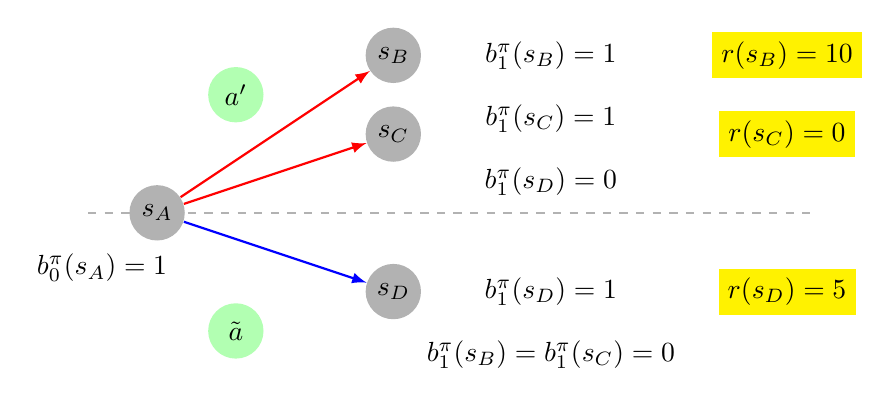
\begin{tikzpicture}
\node (L) at (-1,0) {};
\node (R) at (8.5,0) {};
\draw[thick,dashed,color=black!30] (L) to (R);
\tikzstyle{avertex}=[circle,fill=green!30,minimum size=20pt,inner sep=0pt]
\node[avertex] (a1) at (1,1.5) {$a'$};
\node[avertex] (a2) at (1,-1.5) {$\tilde{a}$}; 

\tikzstyle{vertex}=[circle,fill=black!30,minimum size=20pt,inner sep=0pt]
\node[vertex] (sA) at (0,0) {$s_A$};
\node (b0) at (-0.7,-0.7) {$b^{\pi}_0(s_A) = 1$};
\node[vertex] (sB) at (3,2) {$s_B$};
\node (b1A) at (5,2) {$b^{\pi}_1(s_B) = 1$};
\node[vertex] (sC) at (3,1) {$s_C$};
\node (b1B) at (5,1.2) {$b^{\pi}_1(s_C) = 1$};
\node (b1B) at (5,0.4) {$b^{\pi}_1(s_D) = 0$};
\node[vertex] (sD) at (3,-1) {$s_D$};
\node (b1C) at (5,-1) {$b^{\pi}_1(s_D) = 1$};
\node (b1C) at (5,-1.8) {$b^{\pi}_1(s_B) = b^{\pi}_1(s_C) = 0$};

\node[fill=yellow] (rA) at (8,2) {$r(s_B)=10$};
\node[fill=yellow] (rB) at (8,1) {$r(s_C)=0$};
\node[fill=yellow] (rC) at (8,-1) {$r(s_D)=5$};

\draw[->,>=latex,thick,color=red] (sA) to (sB);
\draw[->,>=latex,thick,color=red] (sA) to (sC);
\draw[->,>=latex,thick,color=blue] (sA) to (sD);
\end{tikzpicture}
\vspace{-0.8cm}
\visible<2->{
\begin{block}{}
% $\mathbb{E}_{s_0 \sim b_0} \croch{ r(s_1) \sachant a_0 = \tilde{a} } = \mathbb{E}_{b_0} \croch{ r(s_1) \sachant a' } = r(s_0) + \frac{\gamma}{2}$. \\
\begin{itemize}
\item $Ch \paren{ r, N_{b^{\pi}_1} \sachant a_0 = \tilde{a} } = r(s_D,\tilde{a}) = 5$, 
\item $Ch \paren{ r, N_{b^{\pi}_1} \sachant a_0 = a' } = \min_{s \in \mathcal{S}} r(s,a') = 0$. \\ 
\end{itemize}
the safe action is prefered! \textbf{dispersion reduced}
\end{block}
}
\visible<3->{	
if $\mathcal{N}_{b^{\pi}_1}$ replaced by $b_1$
$\Rightarrow$ $Ch(r,b_1) = \mathbb{E}_{s \sim b_1} \croch{r(s,a)}$.
% \sum_{s \in \mathcal{S}} r(s,a) \cdot b_1(s)$.
}
\end{frame}
	

\begin{frame}
\frametitle{Choquet integral and rewards}
\framesubtitle{\footnotesize pessimistic evaluation of the rewards -- 
necessity measure}
imprecision of $b^{\pi}$ $=$ agent ignorance $+$ discretization: 
\textbf{pessimistic reward} about these imprecisions.
\visible<2->{
\vspace{-0.15cm}
\begin{alertblock}{Dual measure of $\Pi:2^{\mathcal{S}} \rightarrow \mathcal{L}$}
necessity $\mathcal{N}$ such that
$\forall A \subseteq \mathcal{S}$, $\mathcal{N}(A) = 1 - \Pi(\overline{A})$.
\end{alertblock}
}
\visible<3->{
\vspace{-0.1cm}
%$a \in \mathcal{A}$ fixé:
$r_1 \hspace{-0.1cm} > \hspace{-0.1cm} r_2 > \hspace{-0.1cm} \ldots \hspace{-0.1cm} > \hspace{-0.1cm} r_{k+1} \hspace{-0.05cm}= \hspace{-0.05cm}0$ represents elements of
$\big\{ \hspace{-0.02cm} r(s,a) \hspace{-0.02cm} \big\vert \hspace{-0.02cm} s \in \mathcal{S} \hspace{-0.02cm} \big\}$. %$k \leqslant \# \mathcal{S}$.\\
\vspace{-0.15cm}
\begin{block}{Choquet integral of $r$ with respect to $\mathcal{N}$}
\vspace{-0.6cm}
\begin{eqnarray}
Ch(r,\mathcal{N}) & = & \displaystyle \sum_{i=1}^{k} (r_i - r_{i+1}) \cdot \mathcal{N} \paren{ \set{r(s) \geqslant r_i} }\\
\vspace{-0.1cm}
\visible<4->{
\label{choquet2} & = & \displaystyle \sum_{i=1}^{\# \mathcal{L}-1} (l_i - l_{i+1}) \cdot \hspace{-0.1cm} \min_{ \substack{ s \in \mathcal{S} \mbox{ \scriptsize  s.t. } \\ b^{\pi}(s) \geqslant l_i } }  r(s)
} 
\end{eqnarray}
\end{block}
\vspace{-0.1cm}
\visible<4->{
notation $\mathcal{L} = \set{ l_1=1,l_2,l_3, \ldots, 0 }$.
}
}
\end{frame}

\begin{frame}
\definecolor{violet}{rgb}{0.7,0.1,0.5}
\definecolor{orangee}{rgb}{1,0.7,0.1}
\definecolor{gggreen}{rgb}{0,0.7,0.7}
\frametitle{resulting MDP in practice}
\framesubtitle{\footnotesize trick: ``flipflop'' variable}

\begin{block}{}
boolean variable ``\textit{flipflop}'' $f$ 
changes state at each time step\\ 
$\rightarrow$ defines $2$ phases:
\begin{enumerate}
\item \textit{observation generation}, 
\item \textit{belief update} (deterministic knowing the observation) 
\end{enumerate}
\end{block}
MDP variables:\\ 
\vspace{0.3cm}
$\tilde{\mathbb{S}} =$ \\
 \textbf{beliefs}: \hspace{-0.2cm} $\beta = { \color{violet} \beta^1_v \hspace{-0.05cm} \times \hspace{-0.05cm} \ldots \hspace{-0.05cm} \times \hspace{-0.05cm} \beta^{m_v}_v } \times  { \color{gggreen} \beta^1_h \hspace{-0.05cm} \times \hspace{-0.05cm} \ldots \hspace{-0.05cm} \times \hspace{-0.05cm} \beta^{m_h}_h } \hspace{-0.07cm} \times { \color{orangee} \beta^1_f \hspace{-0.05cm} \times \hspace{-0.05cm} \ldots \hspace{-0.05cm} \times \hspace{-0.05cm} \beta^{m_f}_f } $ \\
\vspace{0.15cm}
\hspace{2cm} $\times$ \\
$ \begin{array}{c} \mbox{\textbf{visible}} \\ \mbox{\textbf{variables}} \end{array} $: $v = f \times { \color{violet} s^1_v \times \ldots \times s^{m_v}_v } \times o_1 \times \ldots \times o_{k} $.
\end{frame}

\begin{frame}
\definecolor{violet}{rgb}{0.7,0.1,0.5}
\definecolor{orangee}{rgb}{1,0.7,0.1}
\definecolor{gggreen}{rgb}{0,0.7,0.7}
\frametitle{resulting MDP in practice}
\framesubtitle{\footnotesize final structured MDP}
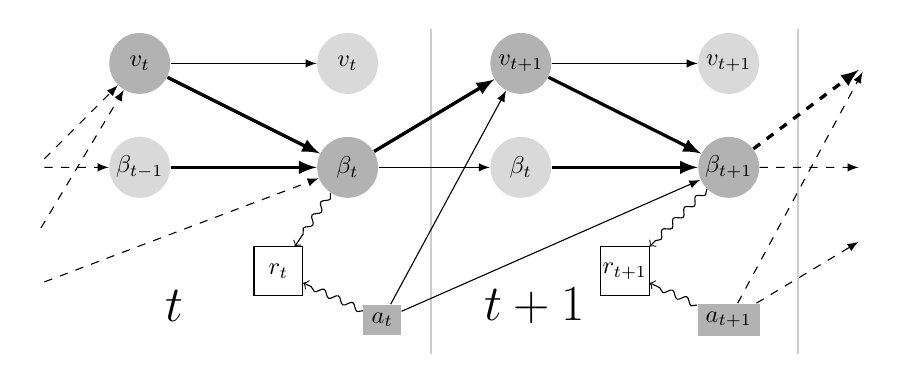
\begin{tikzpicture}[scale=0.88,transform shape]
%%%%%%%%%%%%%%%%%%%%%%%%%%%%%%%%%%%%%%%%%%%%%%%%%%%%%%%%%%%%%%
%TIME/BACKGROUND
\coordinate (middleTop) at (5.7,3);
\coordinate (middleBot) at (5.7,-1.7);
\draw[thick,color=black!20] (middleTop) -- (middleBot);
\node [font=\huge] (statet) at (2,-1) {$t$};
\coordinate (middleTop2) at (11,3);
\coordinate (middleBot2) at (11,-1.7);
\draw[thick,color=black!20] (middleTop2) -- (middleBot2);
\node [font=\huge] (statetplus1) at (7.2,-1) {$t+1$};

%%%%%%%%%%%%%%%%%%%%%%%%%%%%%%%%%%%%%%%%%%%%%%%%%%%%%%%%%%%%%%
%vertex
%vars
\tikzstyle{vertex}=[circle,fill=black!30,minimum size=25pt,inner sep=0pt]
\tikzstyle{vertex2}=[circle,fill=black!15,minimum size=25pt,inner sep=0pt]
\tikzstyle{vertex3}=[ draw, inner sep=0pt, minimum size=20pt]

%1
\node[vertex] (state1) at (1.5,2.5) {$v_t$};
\node[vertex2] (state12) at (1.5,1) {$\beta_{t-1}$};
%1bis
\node[vertex2] (state1bis) at (4.5,2.5) {$v_t$};
\node[vertex] (state12bis) at (4.5,1) {$\beta_t$};
%R1
\node[vertex3] (R1) at (3.5,-0.5) {$r_t$};

%2
\node[vertex] (state2) at (7,2.5) {$v_{t+1}$};
\node[vertex2] (state22) at (7,1) {$\beta_{t}$};

%2bis
\node[vertex2] (state2bis) at (10,2.5) {$v_{t+1}$};
\node[vertex] (state22bis) at (10,1) {$\beta_{t+1}$};
%R2
\node[vertex3] (R2) at (8.5,-0.5) {$r_{t+1}$};

%0
\node (state02) at (0,1) {};
\node (state03) at (0,2) {};
%3
\node (state3) at (12,2.5) {};
\node (state33) at (12,2) {};
\node (state32) at (12,1) {};
\node (state32bis) at (12,0) {};

%action
\node[fill=black!30] (action) at (5,-1.2) {$a_t$};
\node (action0) at (0,0) {};
\node (action02) at (0,-0.7) {};
\node[fill=black!30] (action3) at (10,-1.2) {$a_{t+1}$};

%%%%%%%%%%%%%%%%%%%%%%%%%%%%%%%%%%%%%%%%%%%%%%%%%%%%%%%%%%%%%%
%ARROWS
%1->2
\draw[->,>=latex] (state1) -- (state1bis);
\draw[->,>=latex,very thick] (state1) -- (state12bis);
\draw[->,>=latex, very thick] (state12) -- (state12bis);
%1->2bis
\draw[->,>=latex, very thick] (state12bis) -- (state2);
\draw[->,>=latex] (state12bis) -- (state22);
%0->1
\draw[->,>=latex,dashed] (state02) -- (state1);
\draw[->,>=latex,dashed] (state02) -- (state12);
%2->3
\draw[->,>=latex] (state2) -- (state2bis);
\draw[->,>=latex, very thick] (state2) -- (state22bis);
\draw[->,>=latex, very thick] (state22) -- (state22bis);
%2->3bis
\draw[->,>=latex,dashed, very thick] (state22bis) -- (state3);
\draw[->,>=latex,dashed] (state22bis) -- (state32);

%action
%1
\draw[->,>=latex] (action) -- (state2);
\draw[->,>=latex] (action) -- (state22bis);
\draw[->,decorate,decoration={snake,amplitude=.4mm,segment length=2mm,post length=1mm}] (action) -- (R1); 
%0
\draw[->,>=latex,dashed] (action0) -- (state1);
\draw[->,>=latex,dashed] (action02) -- (state12bis);
%3
\draw[->,>=latex,dashed] (action3) -- (state3);
\draw[->,>=latex,dashed] (action3) -- (state32bis);
\draw[->,decorate,decoration={snake,amplitude=.4mm,segment length=2mm,post length=1mm}] (action3) -- (R2); 

% R
\draw[->,decorate,decoration={snake,amplitude=.4mm,segment length=2mm,post length=1mm}] (state12bis) -- (R1); 
\draw[->,decorate,decoration={snake,amplitude=.4mm,segment length=2mm,post length=1mm}] (state22bis) -- (R2); 
\end{tikzpicture}
\vspace{0.3cm}
$\tilde{\mathbb{S}} =$ \\
\vspace{-0.3cm}
\textbf{beliefs}: \hspace{-0.2cm} $\beta = { \color{violet} \beta^1_v \hspace{-0.05cm} \times \hspace{-0.05cm} \ldots \hspace{-0.05cm} \times \hspace{-0.05cm} \beta^{m_v}_v } \times  { \color{gggreen} \beta^1_h \hspace{-0.05cm} \times \hspace{-0.05cm} \ldots \hspace{-0.05cm} \times \hspace{-0.05cm} \beta^{m_h}_h } \hspace{-0.07cm} \times { \color{orangee} \beta^1_f \hspace{-0.05cm} \times \hspace{-0.05cm} \ldots \hspace{-0.05cm} \times \hspace{-0.05cm} \beta^{m_f}_f } $ \\
\vspace{0.15cm}
\hspace{2cm} $\times$ \\
$ \begin{array}{c} \mbox{\textbf{visible}} \\ \mbox{\textbf{variables}} \end{array} $: $v = f \times { \color{violet} s^1_v \times \ldots \times s^{m_v}_v } \times o_1 \times \ldots \times o_{k} $.
\end{frame}
}
\end{document}
